\documentclass[11pt,twoside,final]{eitExjobb}

%%\usepackage[Text,Num]{LUfonts}%% LU fonts (local file)
%\usepackage{pxfonts}
\usepackage{mathpazo}

% ���
\usepackage[T1]{fontenc}

%% Packages used in the thesis
\usepackage{color}
\usepackage{cite}
\usepackage{amsmath,amsfonts,amssymb}
\usepackage{url}
\usepackage{hyperref}
\usepackage{longtable,multirow}
\usepackage[nottoc]{tocbibind}
\usepackage[toc,page]{appendix}
\usepackage{wrapfig}

\unitlength=1mm

\begin{document}

\Title{Large scale cluster analysis \\ with Hadoop and Mahout}
\Author{Felix Aronsson \\ ada07far@student.lu.se }
\Date{\today}
\Advisor{Yufei Pan}
\Company{Tumblr, Inc.}

\MakeTitlePage

\newpage

\frontmatter
\begin{abstract}
Lorem ipsum dolor sit amet, consectetur adipiscing elit. Aliquam ut ipsum nec
nulla vehicula consectetur. Nulla in sem vitae mauris ornare fringilla. Aenean
luctus erat id nulla aliquet fermentum. Integer non massa gravida, vulputate
enim nec, aliquam velit. Proin sit amet leo nibh. Donec molestie vulputate magna
in tristique. Ut nulla dolor, tempor id justo non, porta tristique nisl. Donec
fermentum dui placerat diam facilisis, eu facilisis metus mollis. Suspendisse id
orci sit amet odio adipiscing faucibus. Fusce consectetur luctus bibendum.
Praesent ligula enim, laoreet id tortor at, lacinia pellentesque mauris. Mauris
porttitor elit porttitor lacus sagittis rhoncus. Nulla adipiscing.
\end{abstract}

\newpage

\section*{Acknowledgements}
I would like to thank Yufei Pan at Tumblr for being my supervisor for the
project, but also for helping me get the project started by telling me who to
talk to, setting up meetings and getting me started with using the
infrastructure there. Beitao Li at Tumblr helped me out with getting already
prepared tag data aggregated from logs, for which I would like to thank him.

I also want to thank my employer, MrFriday AB, and in particular Erik Barkeling
and Jonas Troedsson, for allowing me to work on my project as part of my
employment, but also for taking the first contact with the people at Tumblr
about the project.

Finally, I would like to thanks Anders Ard\"o, associate professor at the
department for Electrical and Information Technology (EIT) at Lund University,
for taking the role as examinator for this project, but also for sparking an
interest in machine learning with his course Web Intelligence and Information 
Retrieval.

\tableofcontents
%\cleardoublepage
\listoffigures
\listoftables
\cleardoublepage

\mainmatter

\chapter{Introduction}
\textit{This chapter aims to}
\begin{itemize}
\itshape
\renewcommand{\labelitemi}{$-$}
\item introduce the reader to the context of the project, and what merit it has
from both a techonological point of view as well as a business point of view,
\item introduce the reader to the goals of the project,
\item present previous works with similar goals as this project, and
\item briefly discuss the tools, technologies and infrastructure used in the
project.
\end{itemize}

\section{Background}
Processing big data is getting more and more interesting from a business sense
and the rate of data generation is increasing every day as more users use
services on the internet, but also data from mechanical processes and sensors
as industries are becoming more and more digitally connected. A 2011 report by
the McKinsey Global Institute estimated that using insights from big data
analysis are not necessarily limited to efficiency and quality improvements in
private coporations, but also for countries and government entities. For
example, they estimate that data from the US health sector has, with creative
and effective use of big data analysis, a potential value of \$300 billion every
year.\cite{manyika2011big}

For social media companies (Facebook, Twitter, Tumblr, et.c.) where
user-generated content is key, being able to process the user data is of course
important.  Facebook, for instance, has a 300 PB data warehouse of
data.\cite{facebookwarehouse} To process such vast amounts of data, the
algorithms used needs to be highly parallelizable.


\begin{wrapfigure}{o}{0.5\textwidth}
  \begin{center}
    
\includegraphics[width=0.48\textwidth]{tumblr_logotype_white_blue.eps}
  \end{center}
\end{wrapfigure}

\subsection{Tumblr}

One of the social media companies with a large amount of user generated data is
Tumblr which this thesis is centered around.  Tumblr (\url{www.tumblr.com}) is a
blogging platform established in early 2007 that currently hosts 170+ million
blogs with 80+ billion posts and is one of the top 30 most visited web sites in
the world.

Each of these 80+ billion posts can be (optionally) tagged with one or more tags
when the user submits the post.  The main data set of this project consists of
the subset of blogs that have used tags in any of their posts combined with the
tags they used and how many times.

Tumblr already has an experienced search team that has developed multiple
features used in production, the most user-noticable of course being the main
search feature. This far, unsupervised clustering has not been extensively used.

\section{Tools, infrastructure and data sets}

\subsection{Hadoop and Mahout}
As described above, processing large amounts of data is becoming more and more
valuable for corporations. Hadoop and the MapReduce paradigm is becoming the
defacto standard for processing large amounts of data as corporate usage
continues to increase.\cite{white2012hadoop}

In 2003 and 2004 Google published two papers introducing the Google File System
(GFS) and Google MapReduce respectively. GFS is a distributed file system
intended to be run on commodity hardware scaling to petabytes of data and Google
MapReduce a framework for running computations on data in GFS.
\cite{dean2008mapreduce,ghemawat2003gfs} 

\begin{wrapfigure}{r}{0.5\textwidth}
  \begin{center}
    
\includegraphics[width=0.48\textwidth]{HadoopLogo.jpg}
  \end{center}
\end{wrapfigure}

The Apache Hadoop project is an open source implementation of the techniques and
ideas presented in the Google papers. The Hadoop Distributed File System (HDFS)
roughly corresponds to GFS while Hadoop MapReduce / YARN is a framework to run
MapReduce-based computations on data in HDFS.\cite{apachehadoop} The Apache
Hadoop project envelops quite a few more related projects but the only one used
in this thesis is Apache Mahout, so the rest are out of scope.

\begin{wrapfigure}{r}{0.5\textwidth}
  \begin{center}
    
\includegraphics[width=0.48\textwidth]{mahout-logo-400.png}
  \end{center}
\end{wrapfigure}

Hadoop does not in it self have any means for performing machine learning tasks,
this is where Mahout comes in. Mahout is a Apache Foundation project that brings
filtering, classification and clustering algorithms to the Hadoop ecosystem.
Apache Mahout implements a number of machine learning algorithms such as
recommenders, classifier training and, the focus of this thesis, cluster
analysis in a parallel manner by utilizing the MapReduce framework and HDFS.
This allows Mahout to horizontally scale to be able to process data sets larger
than a single machine would be able to handle.\cite[pp.~1--6]{owen2011mahout}

\subsection{Hadoop clusters}
The Hadoop framework of course runs on top of a Hadoop cluster. This thesis
project will use two clusters. The first is Amazon's Elastic MapReduce (EMR), a
cloud service for running a Hadoop cluster on their cloud computing platform,
EC2. This allows for scaling up from a tiny one core cluster to more or less
arbitrary sized clusters (in reality there is a limit of 20 nodes for
``unverified'' accounts) which will be of great use for testing the scalability
of Apache Mahout. 

The second Hadoop cluster that will be used is the production
cluster at Tumblr, a cluster consisting of 1900+ cores. Since this is a
production cluster I will not be able to utilize 100\% of it, but it will most
certainly outperform the clusters set up on Amazon's EMR with a wide margin.

\subsection{Data sets}
Finally, the data to be processed consists of two data sets. One compiled from
the music database Last.FM. The data set was created in 2007 and consists of
approximately 20 000 unique artists tagged with 100 000 unique tags (the total
tag count is rougly 7.1 million).\cite{Lamere2010LastFm} 

The second data set is from Tumblr and consists of a snapshot of the activity
across the site for a continous period of time. The data set is large in both
dimensionality, approximately 40 million unique tags, and cardinality,
approximately 12 million blogs. A total of 8 billion tags were used during the
time period.

The Last.FM data set is publicly available for download \cite{Lamere2010LastFm}
whereas the Tumblr data set is proprietary and not available to the public as it
contains user-specific data.

\section{Previous works}
One example of previous works regarding the scaling ability of Mahout are
Ericson and Pallickara of Colorado State University who used a
100 core cluster with the Reuters-21578 data set. This data set consists of
21578 documents and approximately 95000 bigrams.\cite{ericson} 

Another is the book ``Taming Text'' by Ingersol et al. where the authors use a
64 core cluster to cluster a data set consisting of the Apache Software
Foundation mailing lists.\cite{ingersoll} Both these tests are quite a bit
smaller than the proposed tests in this project, both in terms of data set size
and the size of the Hadoop cluster.

\section{Goals and methodology}
The Tumblr data set (which ultimately is the primary data set of this thesis) is
massive in terms of dimensionality (number of tags) and cardinality (number of
blogs). The overall goal of this thesis is to investigate the possibility and
techniques of cluster analysis in a large scale. More specifically using the
Hadoop framework and the Mahout machine learning libraries discussed later.

The main idea of the project is to apply cluster analysis techniques to
this data set by considering each blog as a document and using the tags of
those blog as attributes to calculate the distance to other blogs. First and
foremost, the goal is to see whether or not Mahout is capable of the task of
clustering such high dimensional and large data sets as the Tumblr one.
Secondly, it will be interesting to see what, if any, interesting patterns
emerge from clustering based on used-submitted tags.

First, a survey and discussion of of various algorithms and techniques will be
presented after which a short investigation into the characteristics of the two
data sets will be performed. Using the information found in these tasks, the
Last.FM data set (used here as a small scale test) will be clustered and the
results examined. Finally, using the lessons learned from the small scale tests,
the Tumblr data set will be clustered and the results examined in the same way.

\chapter{Survey}

\textit{This chapter aims to}
\begin{itemize}
\itshape
\renewcommand{\labelitemi}{$-$}
\item present a number of distance metrics used to compare vectors in a vector
space, and
\item discuss a few of the clustering algorithms implemented in Mahout.
\end{itemize}

\section{Distance measures}
In common for a lot of the clustering algorithms discussed later is that a
choice of distance metric needs to be done. Distance between vectors can be
measured in numerous ways depending on the vector space and the nature of the
modelled data.

In this section a number of possible
choices are described, with a focus on those already implemented within Mahout.

\subsection{Distances based on $L^p$-norms}

If the norm of a vector $\vec{u}$ in a vector space $R^n$ is given by

$$
||\vec{u}||_p = \left( \sum_{i=1}^n |u_i|^p \right)^\frac{1}{p}
$$

where $p$ is a real number larger than or equal to 1 we say that it is called a
vector in $L^p$-space over $R^n$. The distance function between two vectors in
this space is then given by 

$$ 
d(\vec{u}, \vec{v}) = \left( \sum_{i=1}^n |u_i - v_i|^p \right)^\frac{1}{p}
$$

By choosing different values for $p$, the distance function and its
characteristics changes. Some common values for $p$ are presented below.

\subsection*{Manhattan distance} 
The distance between two data points computed using the Manhattan distance is
simply the sum of the absolute differences of each dimension of the vectors. The
name comes from the grid-like structure of New York's Manhattan burrough.

The distance is given by the formula

$$
d(\vec{u}, \vec{v}) = \sum_{i=1}^n |u_i - v_i|
$$

This is a distance in a $L_p$-space, more specifically a vector space with 
the $L_1$ norm.

\subsection*{Euclidean distance}
In a $n$-dimensional Euclidean vector space the distance between two points is
given by

$$
d(\vec{v}, \vec{u}) = \sqrt{\sum_{i=1}^n (u_i - v_i)^2}
$$

This is a special case of $L^p$-distance where $p = 2$.

A closely related distance metric is the squared Euclidean distance, which is
useful when distances only needs to be compared to each other, as the square
root is then not necessary, thus making it less computationally expensive.

\subsection*{Chebyshev distance}
The Chebyshev distance defines the distance between two data points as the
greatest difference in any of their dimensions. Chebyshev distance is also
known as the $L_{\infty}$-metric since it is the limit of
the $L_p$-metrics:

$$
d(\vec{u}, \vec{v}) = max(|u_i - v_i|) = \lim_{k \to \infty} \left( \sum_{i=1}^n 
|u_i - v_i|^k \right) ^\frac{1}{k}
$$

\subsection*{Minkowski distance}
In Mahout there is also an implementation of the Minkowski distance. The
Minkowski distance is the generalization of the $L_p$ distances and is, as seen
previously, given by

$$ 
d(\vec{u}, \vec{v}) = \left( \sum_{i=1}^n |u_i - v_i|^p \right)^\frac{1}{p}
$$

We see that for $p = 1$ this equates to the Manhattan distance, for $p = 2$ to
the Euclidean distance and when $p \to \infty $ we have the Chebyshev distance.
This generalization allows the user to specify arbitrary values for $p$ and for
highly dimensional data sets using a large exponent $p$ can give more useful
distances. %TODO: Citation badly needed

\subsection{Cosine similarity}
In the classic vector space model of Information Retrieval, each data point is
modeled as a vector in a vector space with each of the terms of the data set as
a dimension. The similarity between two vectors is then determined by
calculating the angle (or rather, cosine of the angle) between
them.\cite{salton1975}

The cosine similarity between two vectors $\vec{u}$ and $\vec{v}$ in
the data set is given by \cite{baeza1999modern}

$$
sim(\vec{u}, \vec{v}) = \frac{\vec{u} \cdot \vec{v}}{\Vert\vec{u}\Vert \times
\Vert\vec{v}\Vert}
$$

Calculating the cosine similarity is especially effective for very sparse data
(common in, for instance, natural language corpora) as only dimensions where
both vectors have a component larger than zero must be considered.
%TODO: something about norms

\subsection{Tanimoto similarity}
The Tanimoto distance is a distance between two data points with binary
features. Originally it was described in the context of classifying plants by
having a binary vector where each bit corresponded to the presence or absence
of a certain trait in that plant.

The formula for the similarity is \cite{rogers1960computer}

$$
sim(\vec{u}, \vec{v}) = \frac{\vec{u} \cdot \vec{v}}{|\vec{u}|^2 + 
|\vec{v}|^2 - \vec{u} \cdot \vec{v}}
$$

Finally, to return a distance-like metric, where a value of $0$ implies a
perfect match and a value $>0$ a greater distance, the similarity is subtracted
from $1$.

$$
T(\vec{u}, \vec{v}) = 1 - sim(\vec{u}, \vec{1})
$$

\subsection{Mahalanobis distance}
Mahalanobis distance is similar to the Euclidean distance, with the addition of
taking in data correlations into the calculation. The squared Mahalanobis
distance is given by \cite[p.~163]{dillon1984multivariate}

$$
d(\vec{u}, \vec{v}) = (\vec{u} - \vec{v})^\intercal S^{-1} (\vec{u} - \vec{v})
$$

where $S^{-1}$ is the correlation matrix between the two vectors. The
Mahalanobis distance is trivially derived from the squared distance:

$$
d(\vec{u}, \vec{v}) = \sqrt{(\vec{u} - \vec{v})^\intercal S^{-1} (\vec{u} -
\vec{v})}
$$

This formula is also what the MahalanobisDistanceFunction class in Mahout
implements. 

Due to the fact that the distance function includes the correlation matrix, the
distance measure has the advantage over the Minkowski distances by accounting
for correlations between the variables. This could be advantageous in data sets
which have been tokenized into unigrams, as some words will more frequently
follow specific other words. Something that would not be taken into
consideration with, for instance, the euclidean distance.

\section{K-Means clustering}
K-means clustering aims to cluster all data points into one of $k$ classes, for
a fixed value of $k$. Initially, $k$ data points are chosen at random to serve
as the initial cluster centroids. All remaining data points are iterated over
and assigned to their nearest centroid, as determined by a chosen distance
metric (e.g. Euclidean distance). When all data points have been assigned to a
cluster, the centroid is recomputed.\cite{jain1999data} As described by
\cite{baeza1999modern}, the recomputated centroid $\vec{\Delta}_p$ for a given
cluster $c_p$ is given by

$$
\vec{\Delta}_p = \frac{1}{|c_p|} \sum_{\vec{d_j} \in c_p} \vec{d_j}
$$

where $\vec{d_j}$ is a certain document in the cluster $c_p$.
The algorithm iterates until no data points change cluster assignment (or a
given threshold has been acheived) at which point the algorithm has converged.

%TODO: Convergence proof, can be somewhat non-rigorous.

Another version of k-means is sequential (or sometimes referred to as on-line)
k-means, in which the cluster centroid is recomputed after each data point is
assigned. This is also the original version of the algorithm, as described by
MacQueen in 1967\cite{macqueen}.

As one of the most popular clustering algorithms K-Means has quite a few
variations which are covered later in this section.

\section{Canopy clustering}
Canopy clustering tries to speed up the clustering of data set that are both
high dimensional and have a large cardinality by dividing the clustering
process into two subprocesses.\cite{mccallum2000}

First, the data set is divided into overlapping subsets called canopies. This is
done by choosing a distance metric and two thresholds, $T_1$ and $T_2$, where
$T_1 > T_2$. All data points are then added to a list and one of the points in
the list is picked at random. The remaining points in the list are iterated over
and the distance to the initial point is calculated. If the distance is within
$T_1$, the point is added to the canopy. Further, if the distance is within
$T_2$, the point is removed from the list. The algorithm is iterated until the
list is empty.\cite{mccallum2000}

The second step of the process is to run another clustering algorithm in these
smaller canopies, often k-means with the canopies as initial centroids.

Canopy clustering can also help the user to estimate the value of $k$ for use in
K-means. Given good threshold values for $T_1$ and $T_2$, canopy clustering will
find a suitable number of canopies. These can, as mentioned, be used as the
initial centroids in a K-means clustering.

McCallum, Nigam and Ungar (2000) also found that using canopy clustering as an
initial step can lead to significant speed-ups in the second clustering
step.\cite{mccallum2000}

\section{Latent dirichlet allocation}
Latent Dirichlet allocation, LDA, works from the assumption that each document
is generated by drawing words from a mixture of latent topics, where the mixture
is individual for the document but the topics are a fixed set. The topics are in
turn characterized by a distribution of the words in the corpus

Using this assumption, a document would be generated by choosing a number of
words in the document from a Poisson distribution, $N \sim Po(\zeta)$ and topic
mixture from the fixed set of $k$ topics, $\Theta \sim Dir(\alpha)$ where
$\alpha$ is a $k$-dimensional vector of real values representing the weight of
each topic.

Each of the $N$ words, $w_n$, are then chosen from a topic (in turn chosen from
the topic mixture of the document). $w_n \sim Mult(\beta)$ where $\beta$ is a
vector of word weights within that topic.

Using Bayesian inference and the generative modeled described, LDA backtracks
to find the topics and mixtures that could generate the
corpus.\cite{blei2003lda}

Mahout uses collapsed variational bayes inference, CVB, to implement LDA. CVB
is more performant as better suited for parallelization\cite{mahout-897}. CVB
uses techniques from both Gibbs sampling, which Mahout previously implemented,
and variational bayes, leading to a more efficient and accurate algorithm
\cite{teh2006collapsed}.

\section{K-Means variations}

\subsection{Spherical k-means clustering}

If instead of the Euclidean distance metric the cosine similarity is used to
calculate distance between data points the variation is usually called
spherical k-means. 

Each document is then represented by a vector to the unit $n$-sphere (hence the
name) where the similarity of two vectors is given by the angle between them.
This has the advantage of only having to consider features that are non-zero in
both vectors. This is advantageous in high-dimensional but sparse data
sets.\cite{dhillon2001}

\subsection{Fuzzy c-means}
Fuzzy c-means is sometimes called fuzzy k-means due to its similarity with
k-means \cite{nock2006weighting}. In fuzzy c-means, each document is assigned to
a multitude of clusters, each with a coefficient describing the degree of the
assignment to that cluster.

Initially, like in k-means clustering, number $k$ of clusters is chosen. Each
document is then assigned a random number representing the degree of assignment
to each cluster. A centroid is calculated for each cluster, where the centroid
is the mean of all documents' assigned coefficient for that cluster.

$$
c_k = \frac{\sum_x w_k(x)^m x}{\sum_x w_k(x)^m}
$$

$w_k(x)$ gives the coefficient (or weight) of a document $x$ in the $k$th
cluster and $m$ is a parameter to the algorithm controlling the importance of
the closest center to a document in recalculating the coefficients for that
document. If $m$ is close to 1 the closest centroid will dominate other
centroids.

% TODO: Try to find "Pattern recognition with fuzzy objective function algorithms"

\subsection{K-medoids}

With normal k-means clustering the mean of the points in each cluster is
assigned as the new centroid, whereas with k-medoids data points are used as the
centroids. $k$ data points are chosen as initial centroids, and when choosing
new centroids the data point which minimizes the sum of distances to all other
data points assigned to the cluster is chosen as the new centroid.

This means that instead of a cluster centroid being defined by a vector in the
vector space, it is defined by on of the data points in the data set.

\chapter{Data set exploration}

\textit{This chapter aims to}
\begin{itemize}
\itshape
\renewcommand{\labelitemi}{$-$}
\item investigate and present the properties of the two data sets
\end{itemize}

Before clustering, it can be useful to explore the data sets to discover their
properties. One common method is to plot the number of occurences of the words
in the corpus against the rank (how common the word is) in a log-log plot.

\begin{figure}[htbp]
  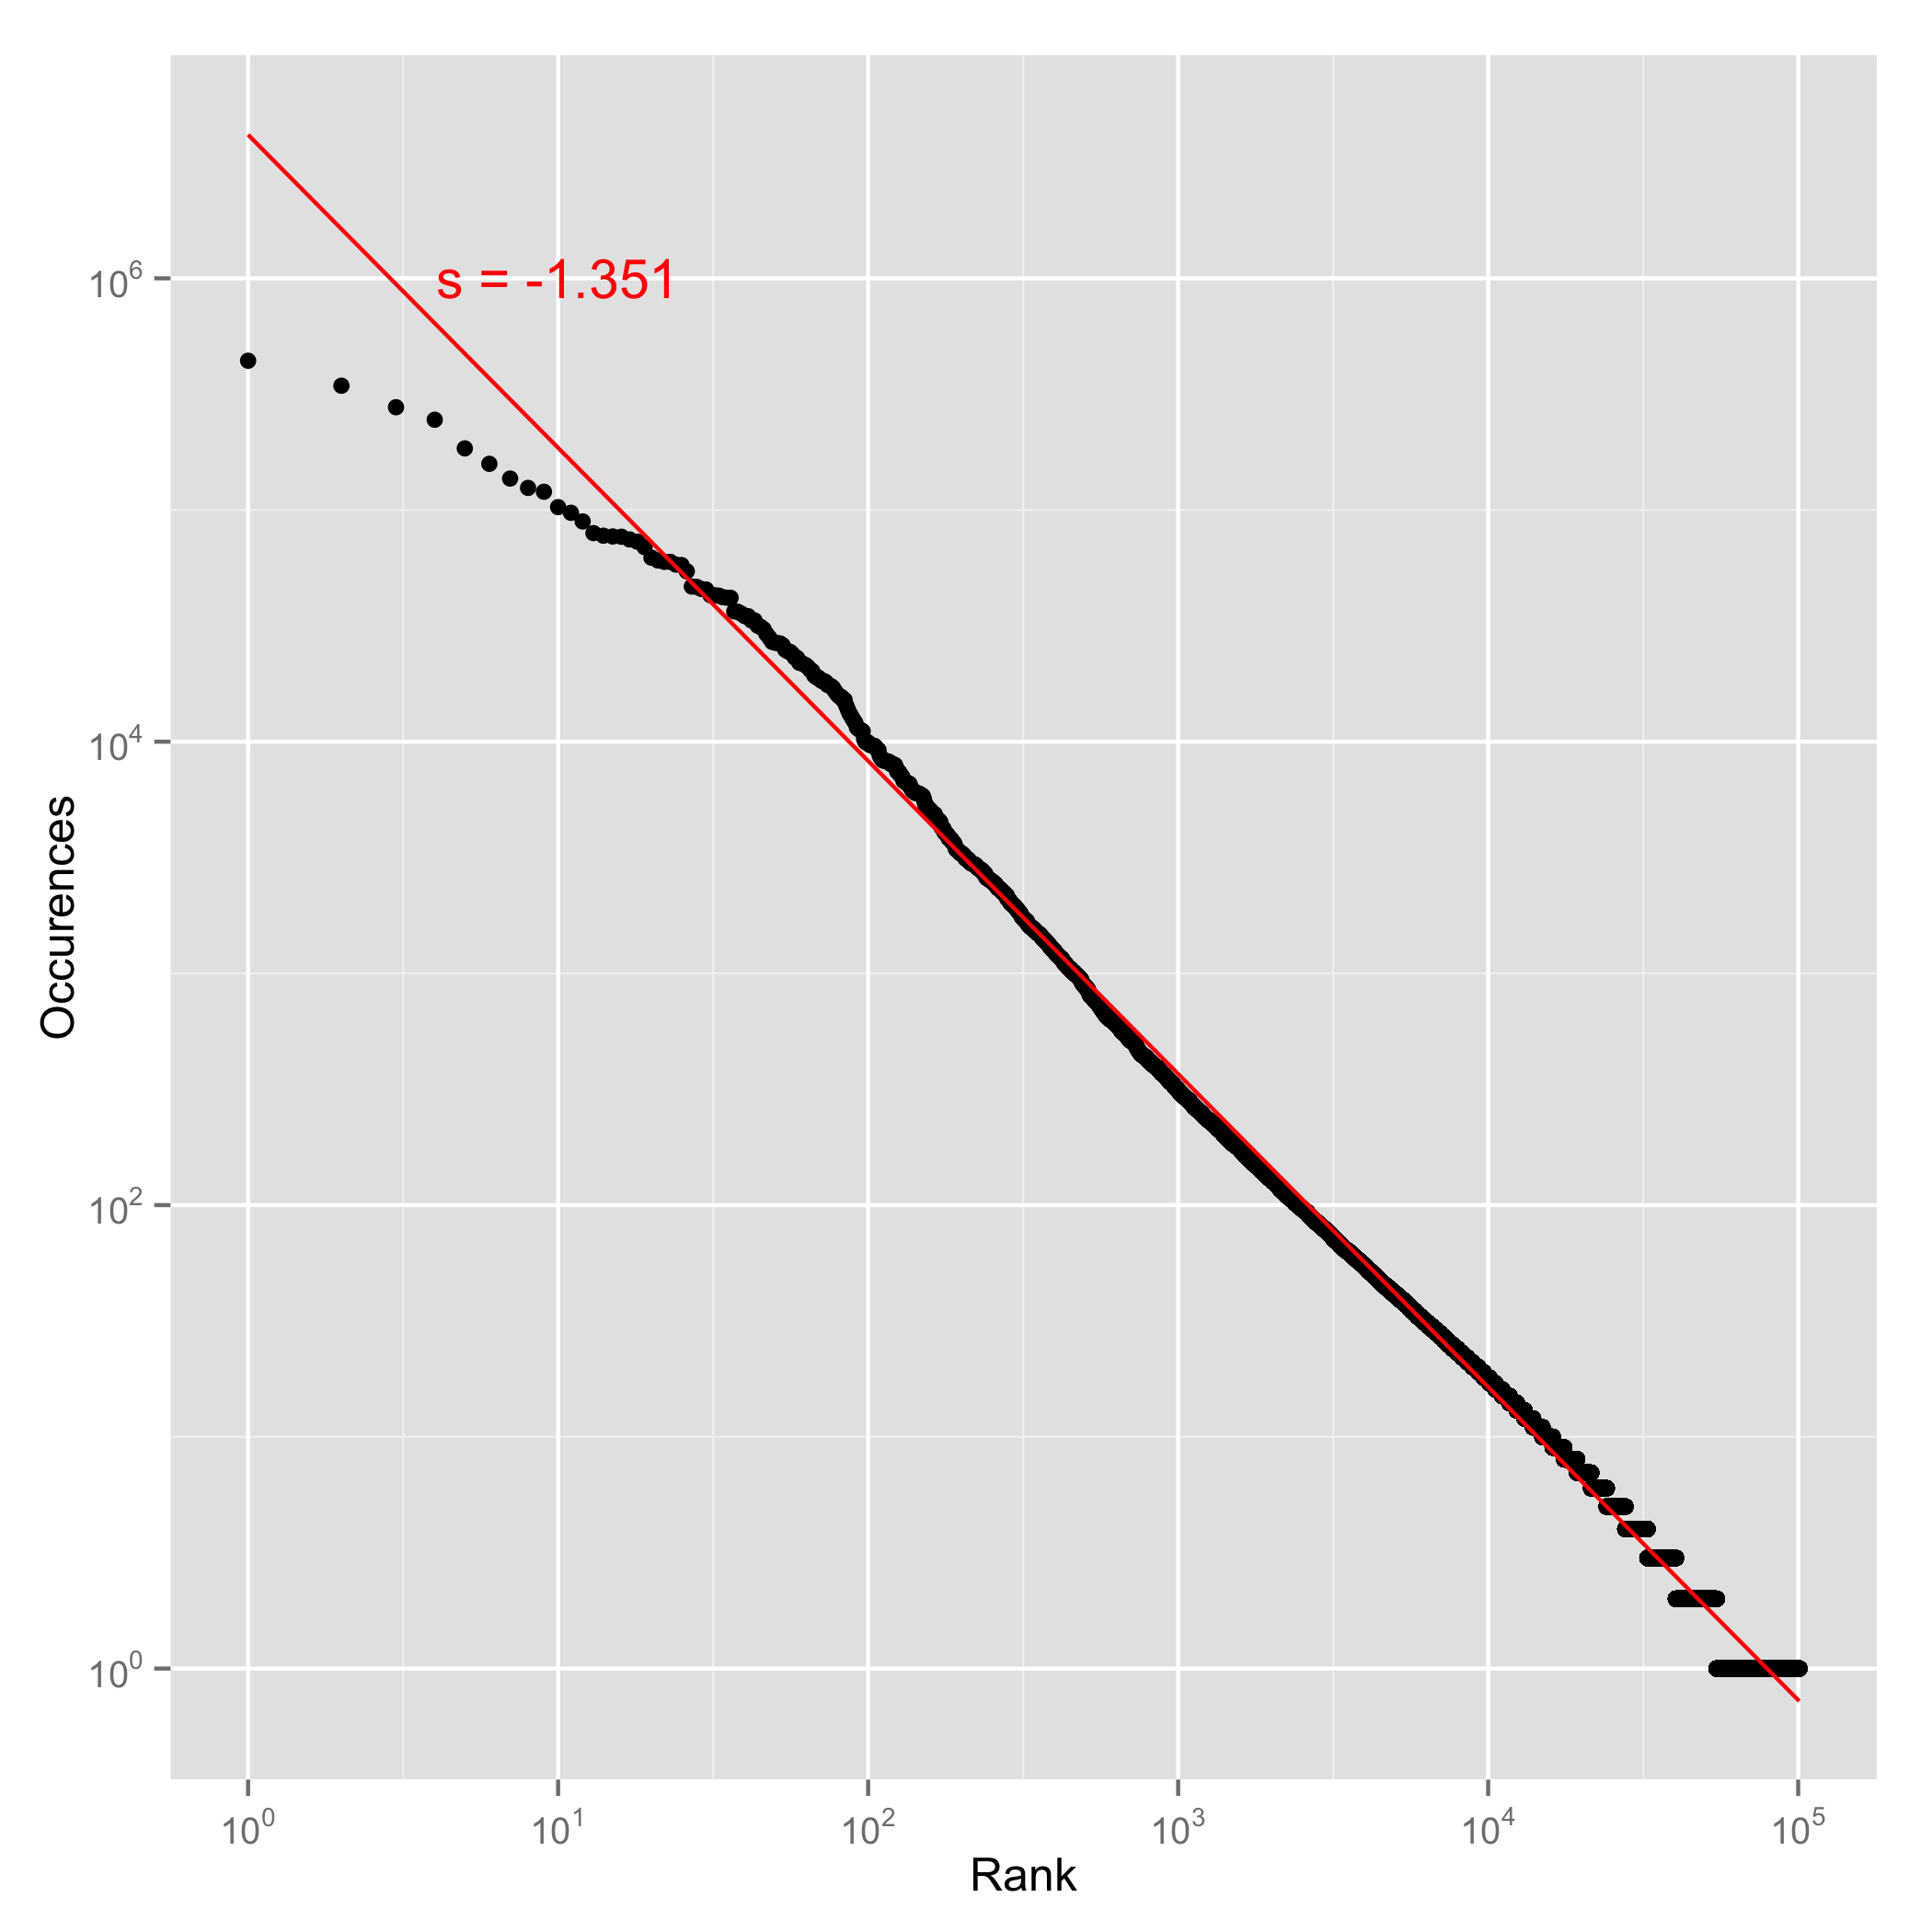
\includegraphics[width=0.7\textwidth]{lastfmzipf.png}
  \centering
  \caption{Tag occurences in the Last.FM data set plotted against the rank}
  \label{fig:lastfmzipf}
\end{figure}

In \autoref{fig:lastfmzipf} the Last.FM data set has been plotted in this
manner. A linear regression has been fitted to the data and shows that lower
ranked tags seem to follow a Zipfian distribution. However, higher ranked tags
deviate somewhat from the regression line. In a natural language corpus (i.e.
not a corpus of tags as this data set) we expect the slope, $s$, to be $-1$ as
empirically determined by Zipf. In the Last.FM data set the slope is $-1.351$,
implying an even longer long tail than in a ``regular'' natural language corpus.

Plotting the Tumblr data set in the same manner gives the scatter plot in
\autoref{fig:tumblrzipf}.

\begin{figure}[htbp]
  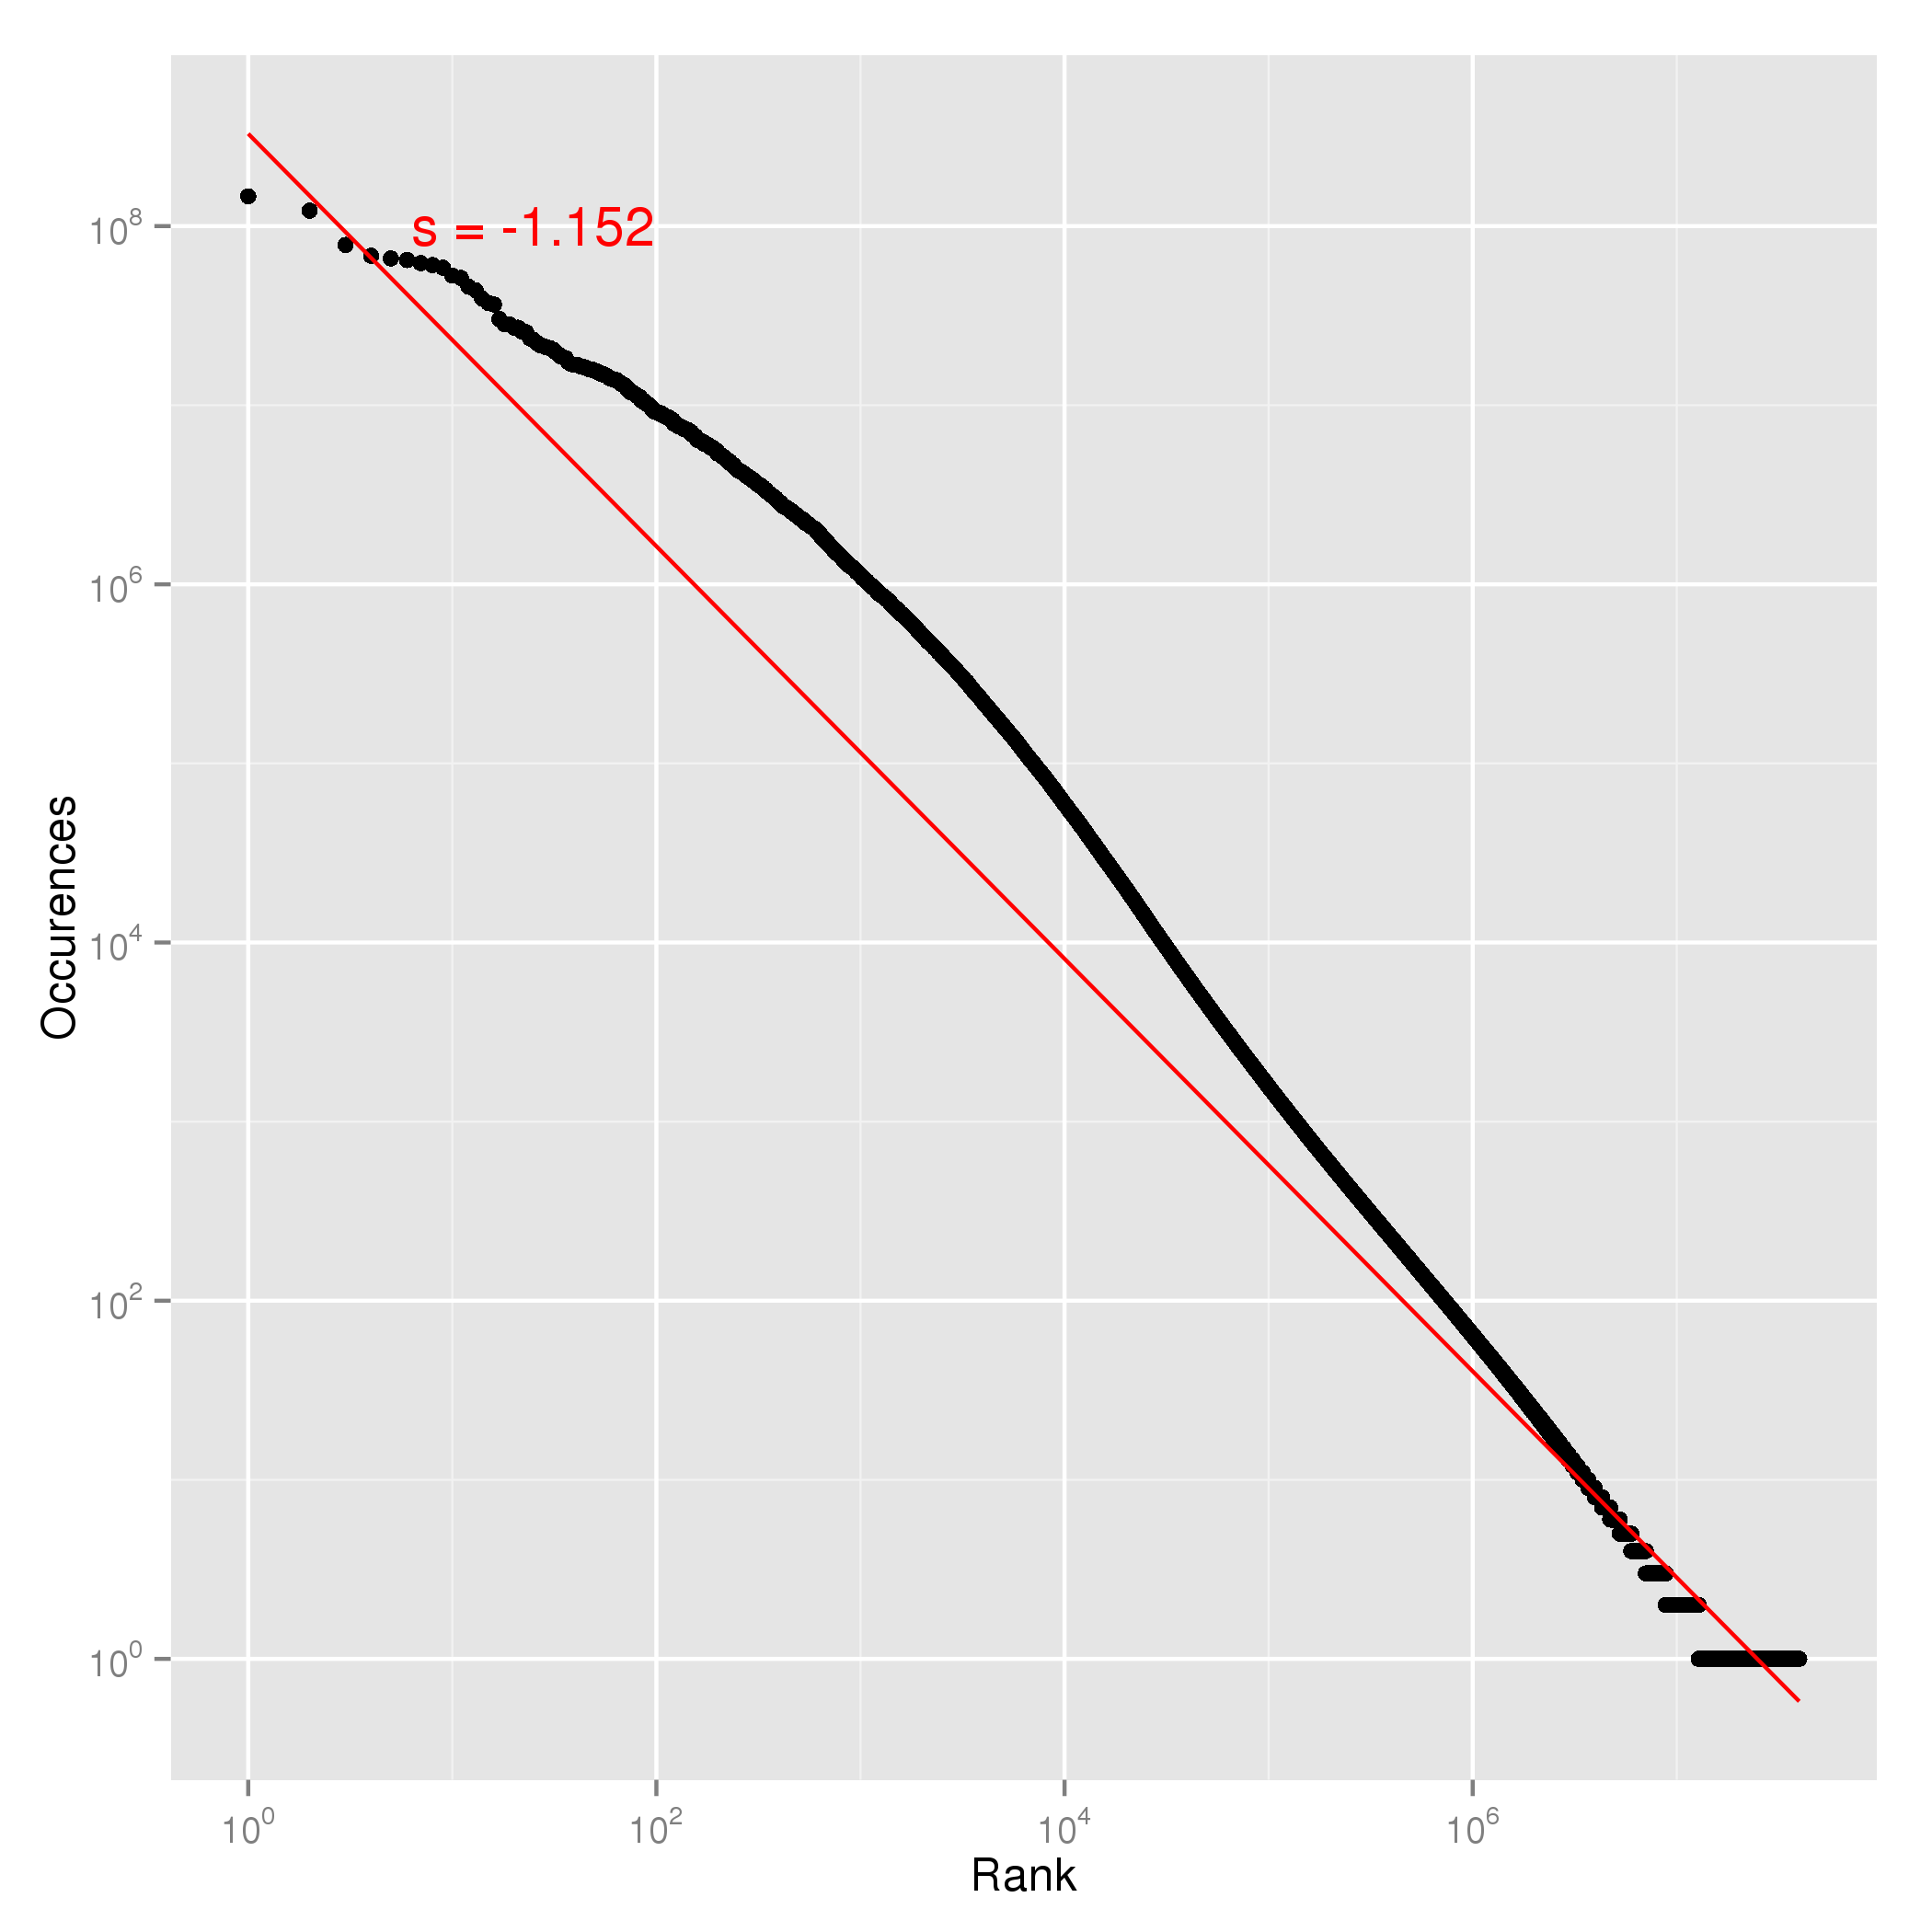
\includegraphics[width=0.7\textwidth]{tumblrzipf.png}
  \centering
  \caption{Tag occurences in the Tumblr data set plotted against the rank}
  \label{fig:tumblrzipf}
\end{figure}

In this case, the slope $s$ is -1.152, a lot closer to to the original
Zipf-distribution. However, the data does not fit the regression line as well as
the Last.FM data set. Although the tail is long, the data is not quite as skewed
as one would expect from a Zipfian distribution.

Another interesting feature to study is what the distribution of amount of tags
per blog looks like. Hypothesizing that this approximately follows a power-law
we again construct a log-log plot, but instead we plot the amount of blogs with
a certain number of tags. The resulting plot for the Last.FM data set can be
seen in \autoref{fig:lastfmpower} and for the Tumblr data set in
\autoref{fig:tumblrpower}.

\begin{figure}[htbp]
  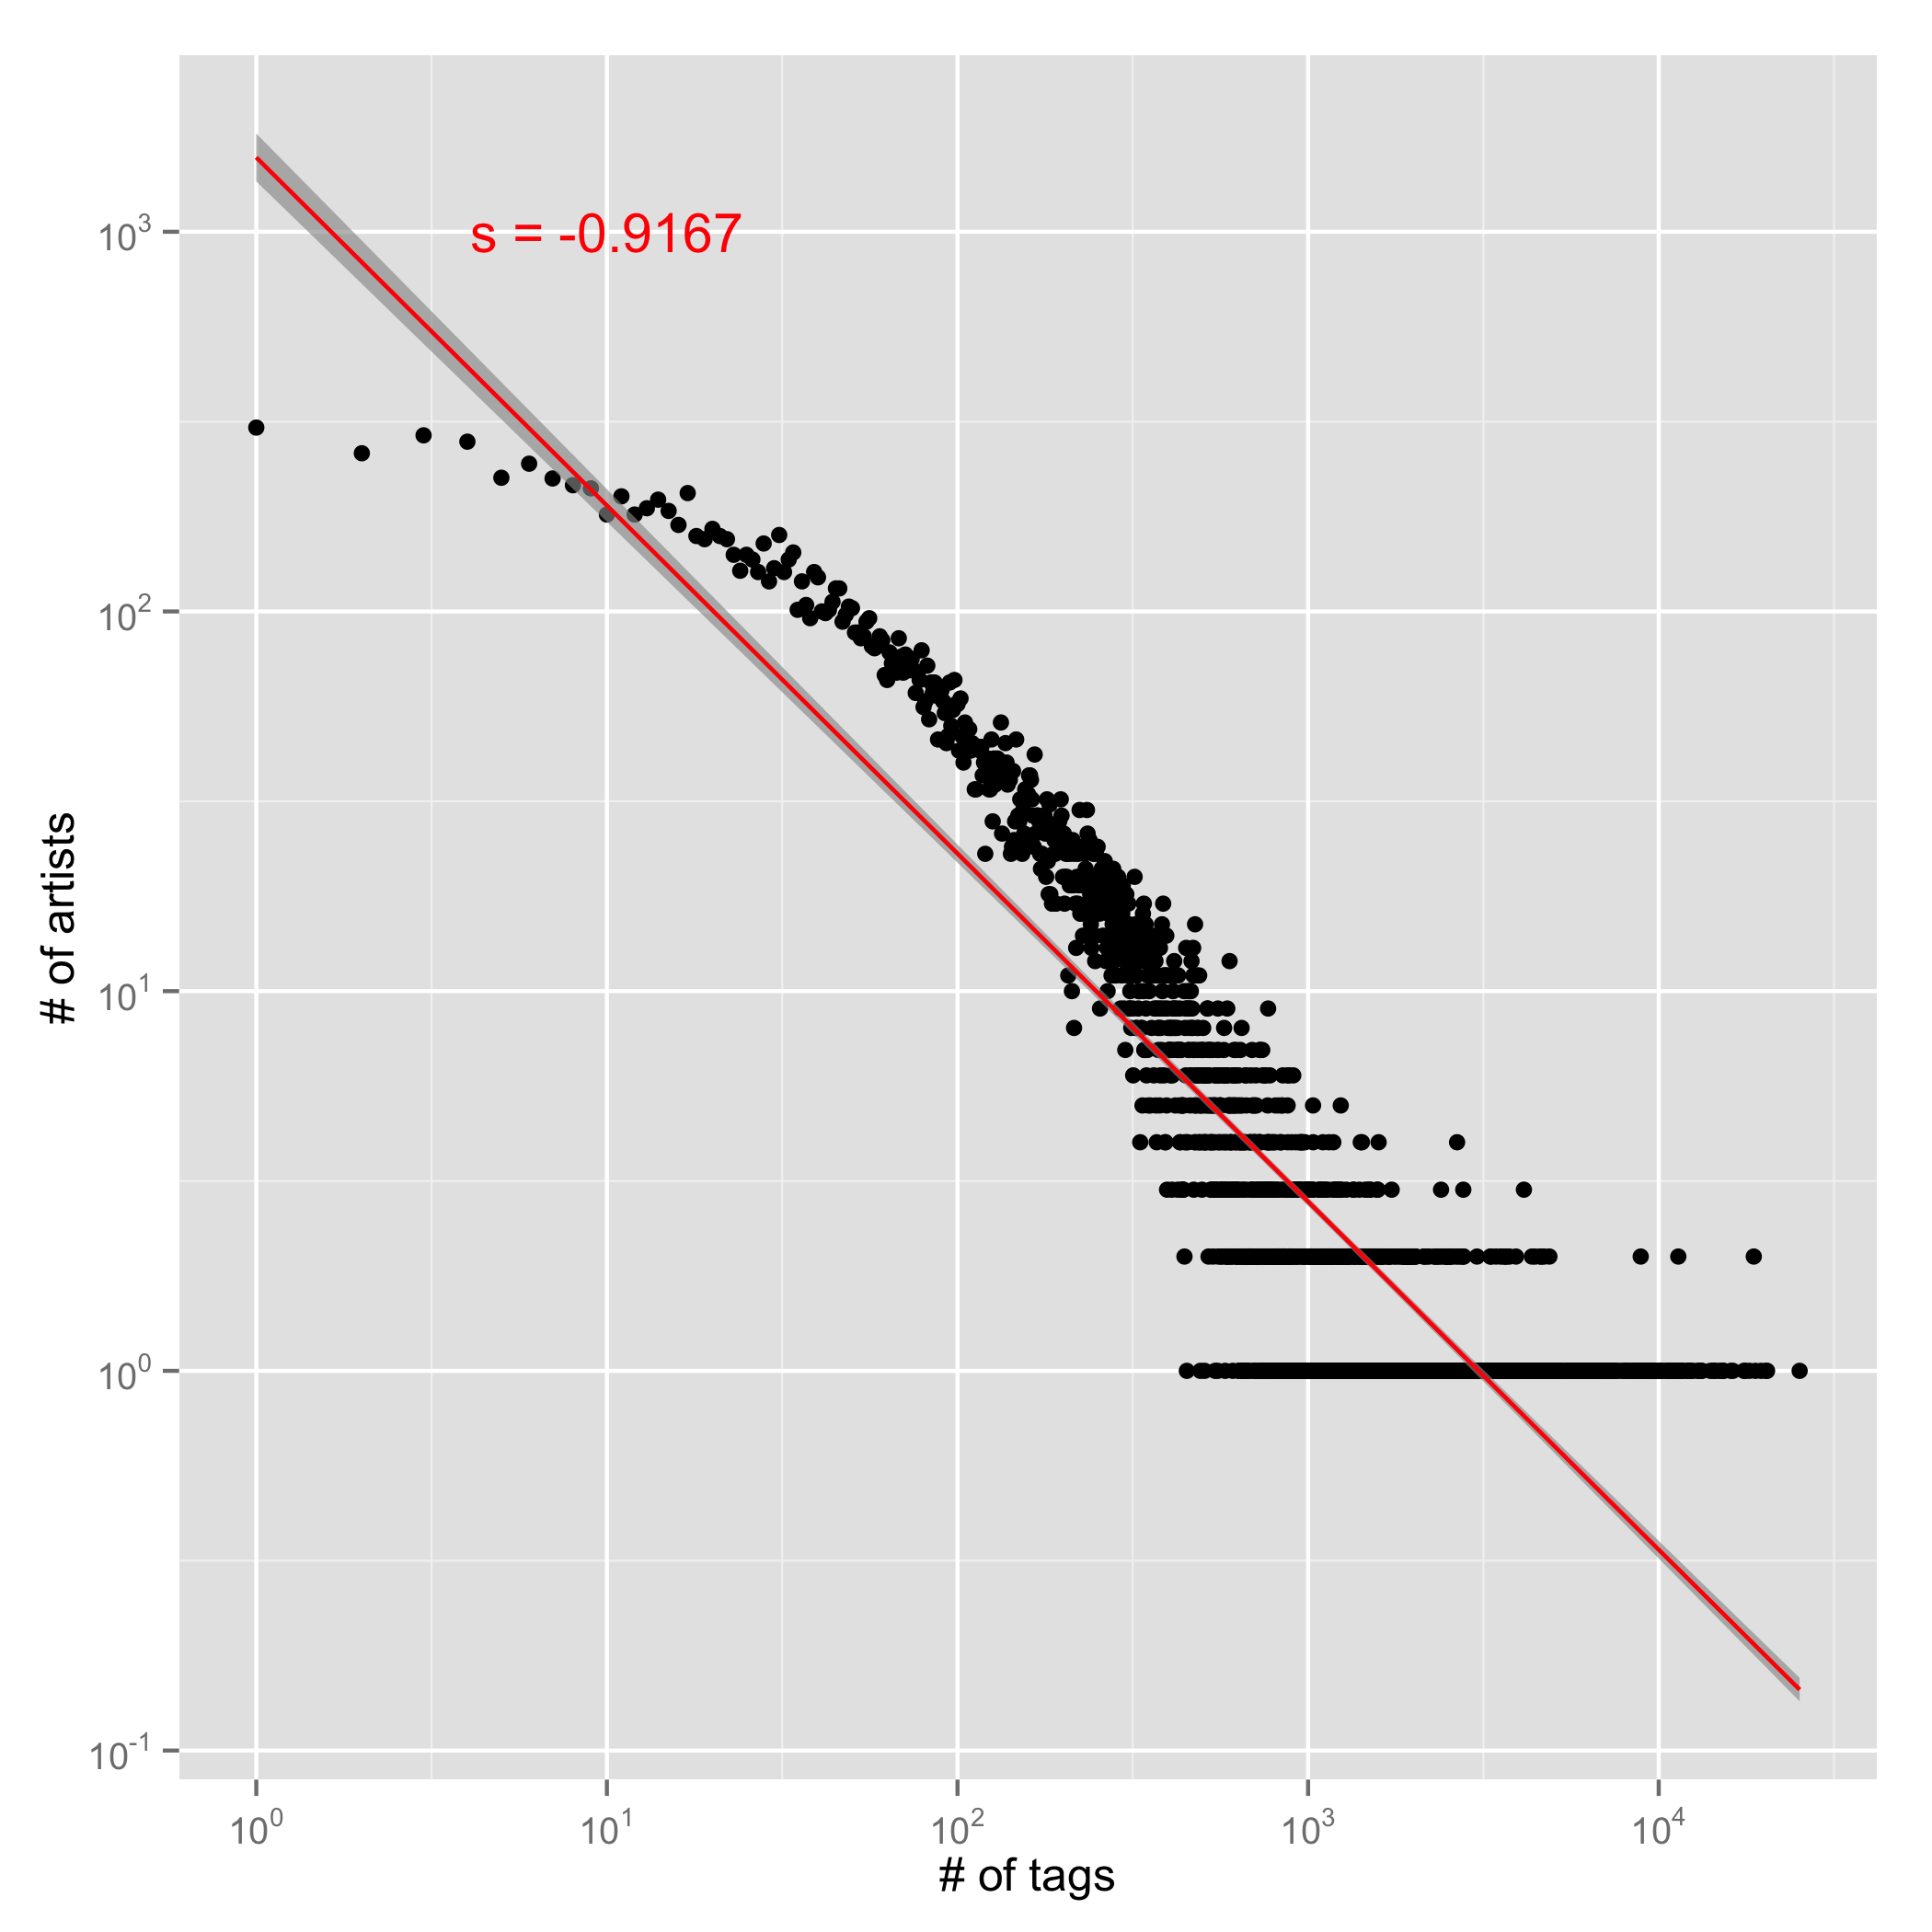
\includegraphics[width=0.7\textwidth]{lastfmpower.png}
  \centering
  \caption{Number of tags per artist (log-log)}
  \label{fig:lastfmpower}
\end{figure}

\begin{figure}[htbp]
  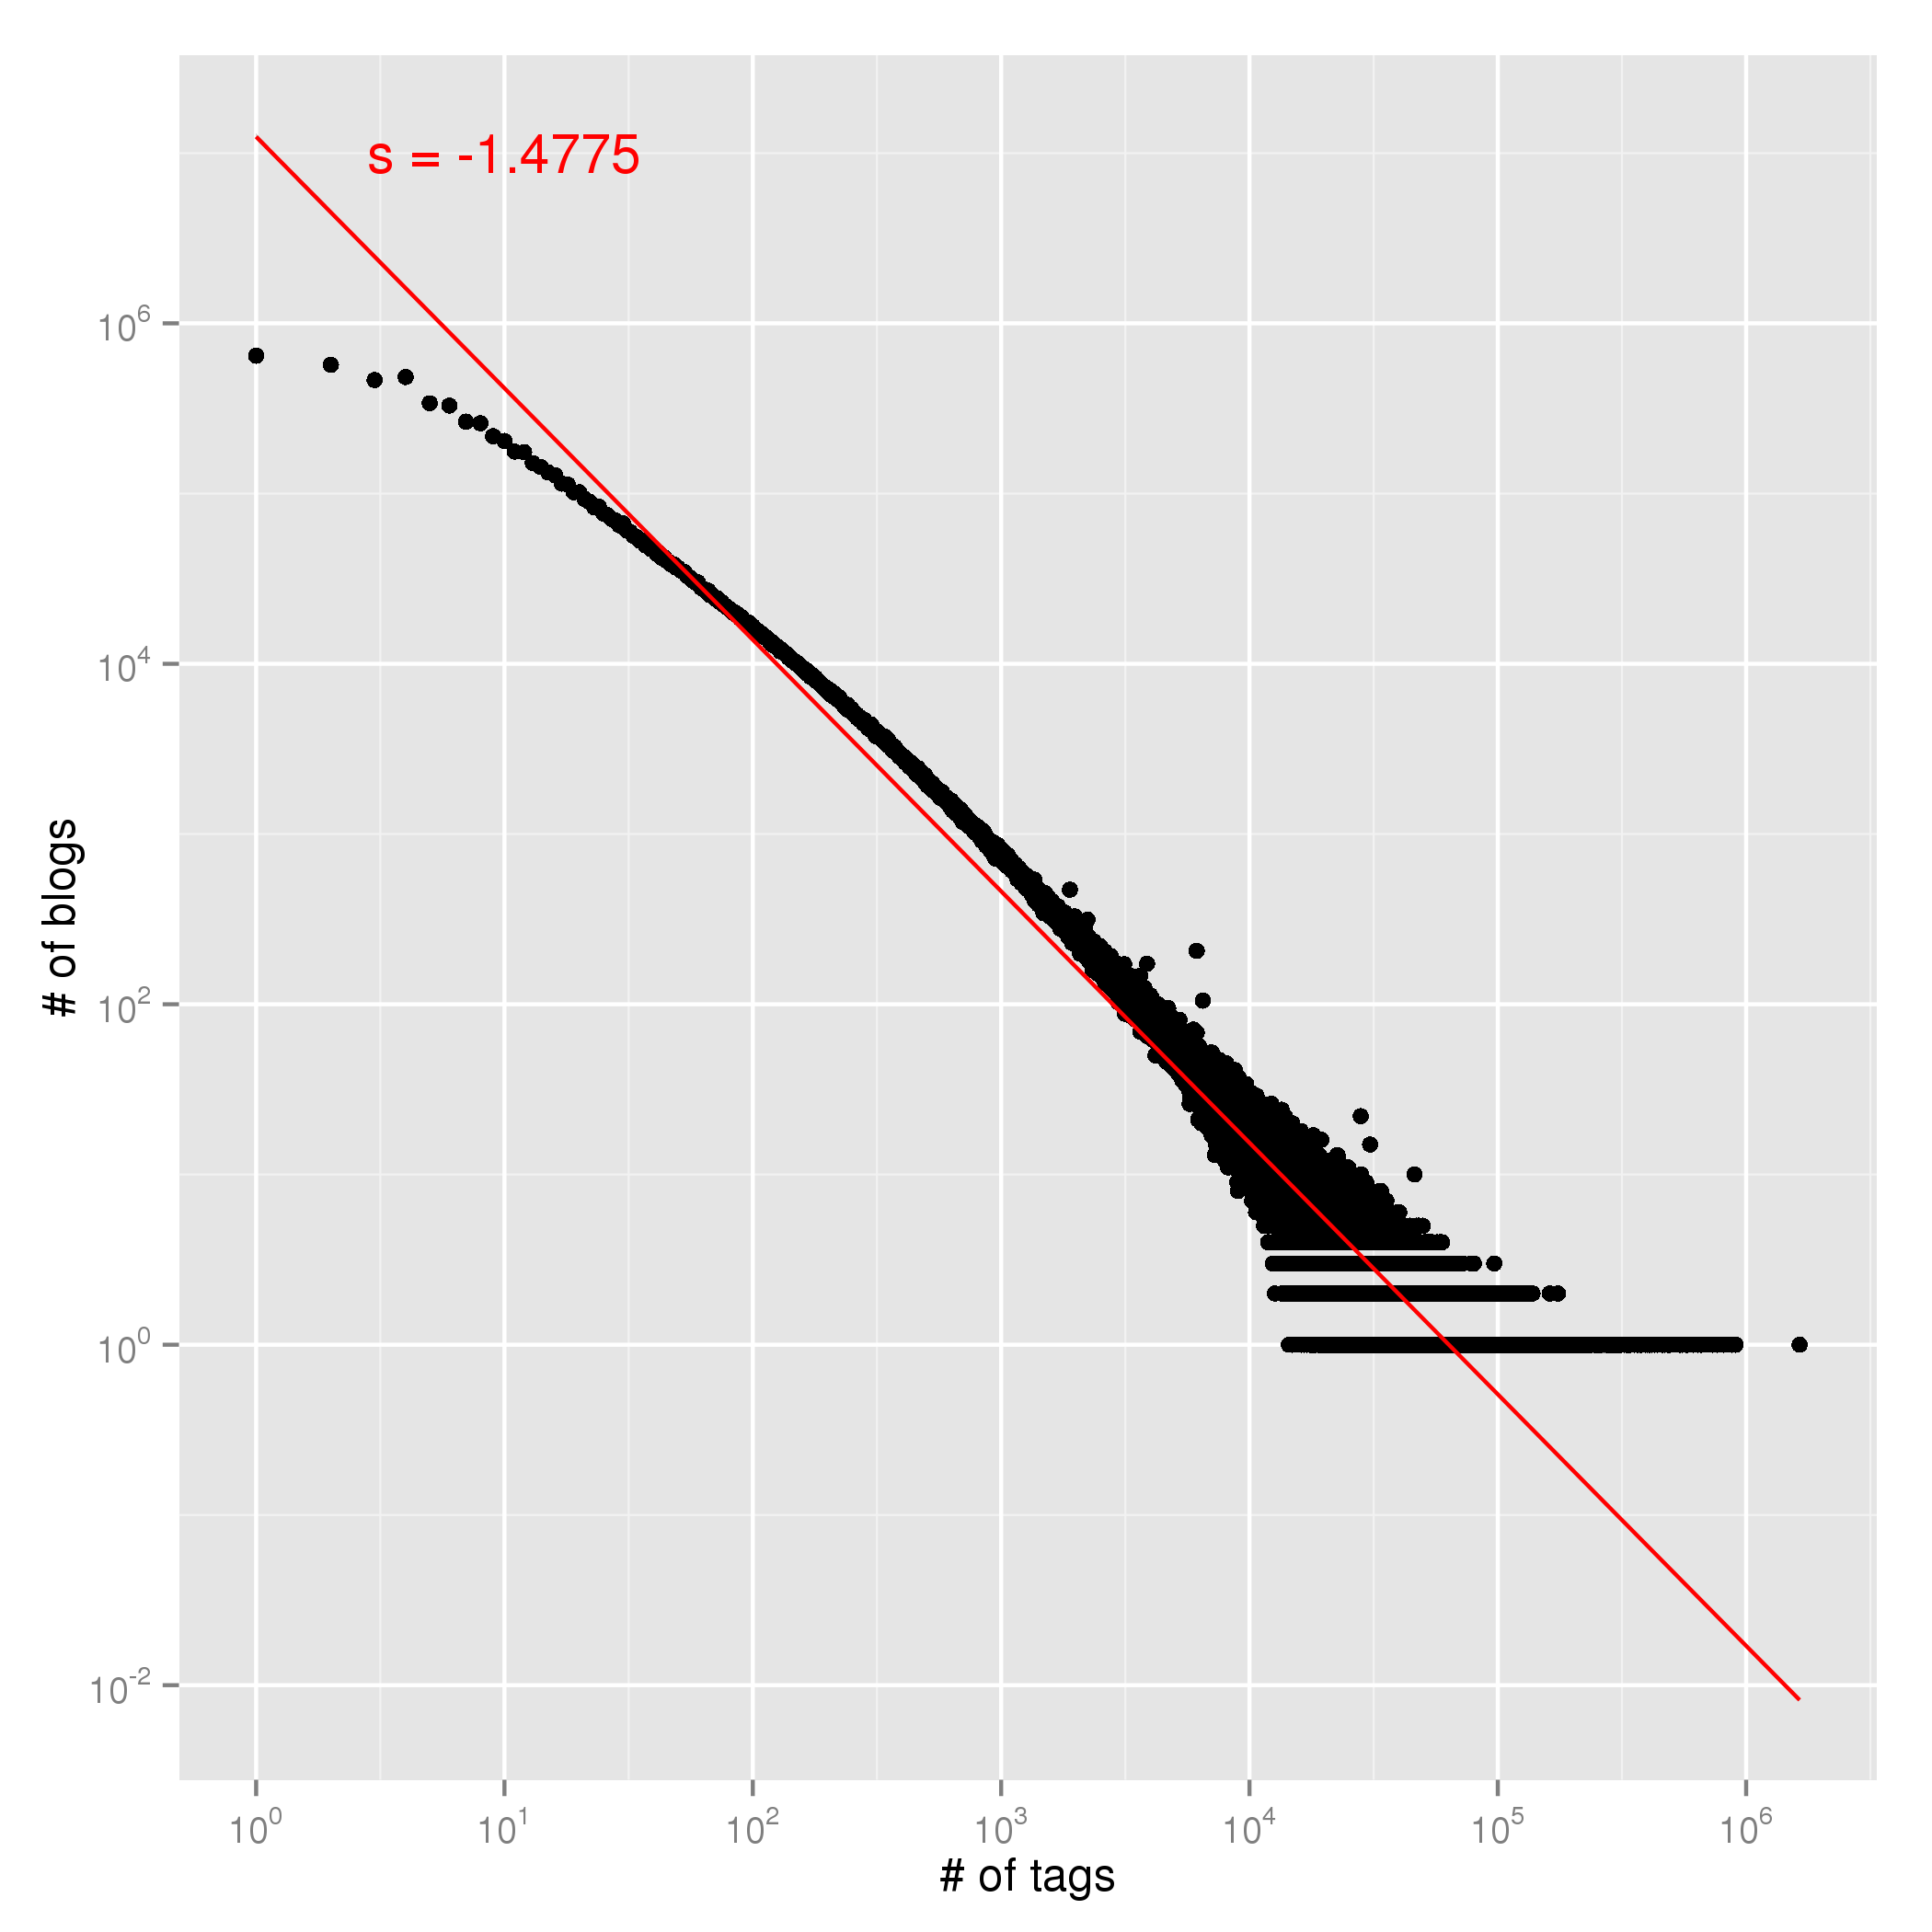
\includegraphics[width=0.7\textwidth]{tumblrpower.png}
  \centering
  \caption{Number of tags per blog (log-log)}
  \label{fig:tumblrpower}
\end{figure}

The tags user per blog in the Tumblr data set follows a power law with the
exponent -1.4775 while the Last.FM data set is less skewed in this regard with
an exponent of -0.9167. One reason for the fact that the Tumblr data set seems
to follow a power law more closely could be that it is tokenized into unigrams,
whereas the Last.FM data set is not. This could also explain the relative
infrequency of the most popular tags in the Last.FM data set. The most popular
genres are often divided into subgenres. For example, ``rock'' has numerous
subgenres such as ``indie rock'', ``country rock'' and ``hard rock''.

\section{Summary}
The data set exploration showed that our data sets does not quite follow
the Zipfian distribution usually seen in natural language data sets.
They are however not very far from the expected distributions and are heavily
skewed (to the point where if not plotted on a log-log scale they are almost a
perfect L-shape), which suggest that techniques normally used for natural
language corpora could work well in these data sets as well.


\chapter{Small scale clustering}

\textit{This chapter aims to}
\begin{itemize}
\itshape
\renewcommand{\labelitemi}{$-$}
\item apply the algorithms and techniques discussed in section 2 to the Last.FM
data set,
\item briefly describe the process of generating TF and TF-IDF weighted feature
vectors from the Last.FM data set,
\item investigate how the performance characteristics of those algorithms depend
on dimensionality, cardinality and number of worker nodes, and
\item present and discuss the outcome of the clustering jobs.
\end{itemize}

\section{Preparation}
Mahout uses a special Vector data structure for representing documents with
feature vectors. There are a few implementations of the AbstractVector class
that can be used. Examples are DenseVector for dense data (mostly non-zero
elements) and two classes for sparse vectors (few non-zero elements),
SequentialAccessSparseVector and RandomAccessSequentialVector. The data sets
used in this project are very sparse and to optimize the distance calculations
the choice ends up on SequentialAccessSparseVector.

The first step taken is to generate a dictionary (a map from tag to an integer
id) of unique tags. In order to do this a MapReduce job to output a list of
unique terms is run. In the map phase, the job takes a line from the input file
and emits the tuple (\textless tag\textgreater, 1). The reduce step takes these
tuples and de-duplicates them by again outputing (\textless tag\textgreater,
1). This list of unique tags is then turned into a dictionary simply by
iterating over each tag while incrementing an integer. This is the only step
that needs to be done sequentially, but it fast enough to process the Last.FM
data set in a few seconds.

To calculate the weights (TF or TF-IDF in this case) two MapReduce jobs are run.
The first calculates the count of a certain tag for a certain artists (e.g. 
``Johnny Cash has been tagged with country $n$ times''). The map phase simply
parses the artist name, tag name and tag count from the input file and emits
a tuple, (\textless artist\textgreater, \textless tag\textgreater;\textless tag
count\textgreater). The reduce phase outputs a tuple for each artist-tag couple
with the associated tag count, but also the total tag count for that artist. The
second step takes the tag count and total tag count and calculates the TF, IDF,
TF-IDF and the raw term frequency according to the following formulas

$$
tf = \frac{n_i}{n_k}
$$
$$
idf = \log \left( \frac{N}{|{ d \in D : w \in d}|} \right)
$$
$$
tfidf = tf \cdot idf
$$

where $n_i$ is the count of a certain tag for a certain artist, $n_k$ is the
total tag count for that artist and $N$ is the total number of artists. The raw
term frequency mentioned above is simply $n_i$, not divided by $n_k$. $D$ is the
set of all artists and the divisor in the IDF-calculation is therefore the total
number of artists tagged with the tag $w$.

Finally, to create the actual feature vectors, a last MapReduce job is run. In
the configuration to this job we include a serialized version of the dictionary.
The map phase then creates partial vectors for each of the artist-tag couples
from the output of the previous step. Each partial vector has the calculated
weight set in the element with index taken from the artist-to-integer mapping
from the dictionary. The reduce phase then combines the partial vectors to a
single, full vector for each artist.

An important thing to note is that the limit (mapred.user.jobconf.limit) for
the configuration is five MB by default. This is enough to contain the
dictionary for the Last.FM data set, but will cause problems for larger data
sets as will become evident in the large scale tests of this project.
 
\section{Spherical k-means}
As mentioned previously, spherical k-means clustering is the process of
clustering a data set using the k-means algorithms with the cosine similarity.
As seen in the data set exploration section, the data sets do not strictly
follow the Zipfian distribution usually seen in natural language, but they are
quite close. As a result, TF/IDF weighting will be used for the spherical
k-means clustering.

\subsection{Determining $k$}
As mentioned before, a successful clustering using k-means depends on the
choice of $k$, the number of clusters. There are several ways of determining
this. One way is the previously mentioned canopy clustering, which is a more
lightweight clustering process that can be used for generating the initial
clusters for k-means, instead of picking them at random.

Another possibility is to run the k-means algorithm multiple times while varying
$k$. The traditional procedure is to inspect the within-cluster sum of squares,
$WSS$, at each $k$. The idea is to find the point where the rate of decrease in
$WSS$ levels out, meaning that for each increase in $k$ the decrease in $WSS$ is
no longer a big ``win''. This method is sometimes called ``the elbow method''.

Mahout provides a simple way to extract the inter-cluster density with its
clusterdump tool. This is the average distance between each of the cluster
centers. An inter-cluster density approaching 1 (when using cosine similarity)
indicates evenly spaced clusters.\cite[pp.~188--190]{owen2011mahout}

\begin{figure}[htbp]
  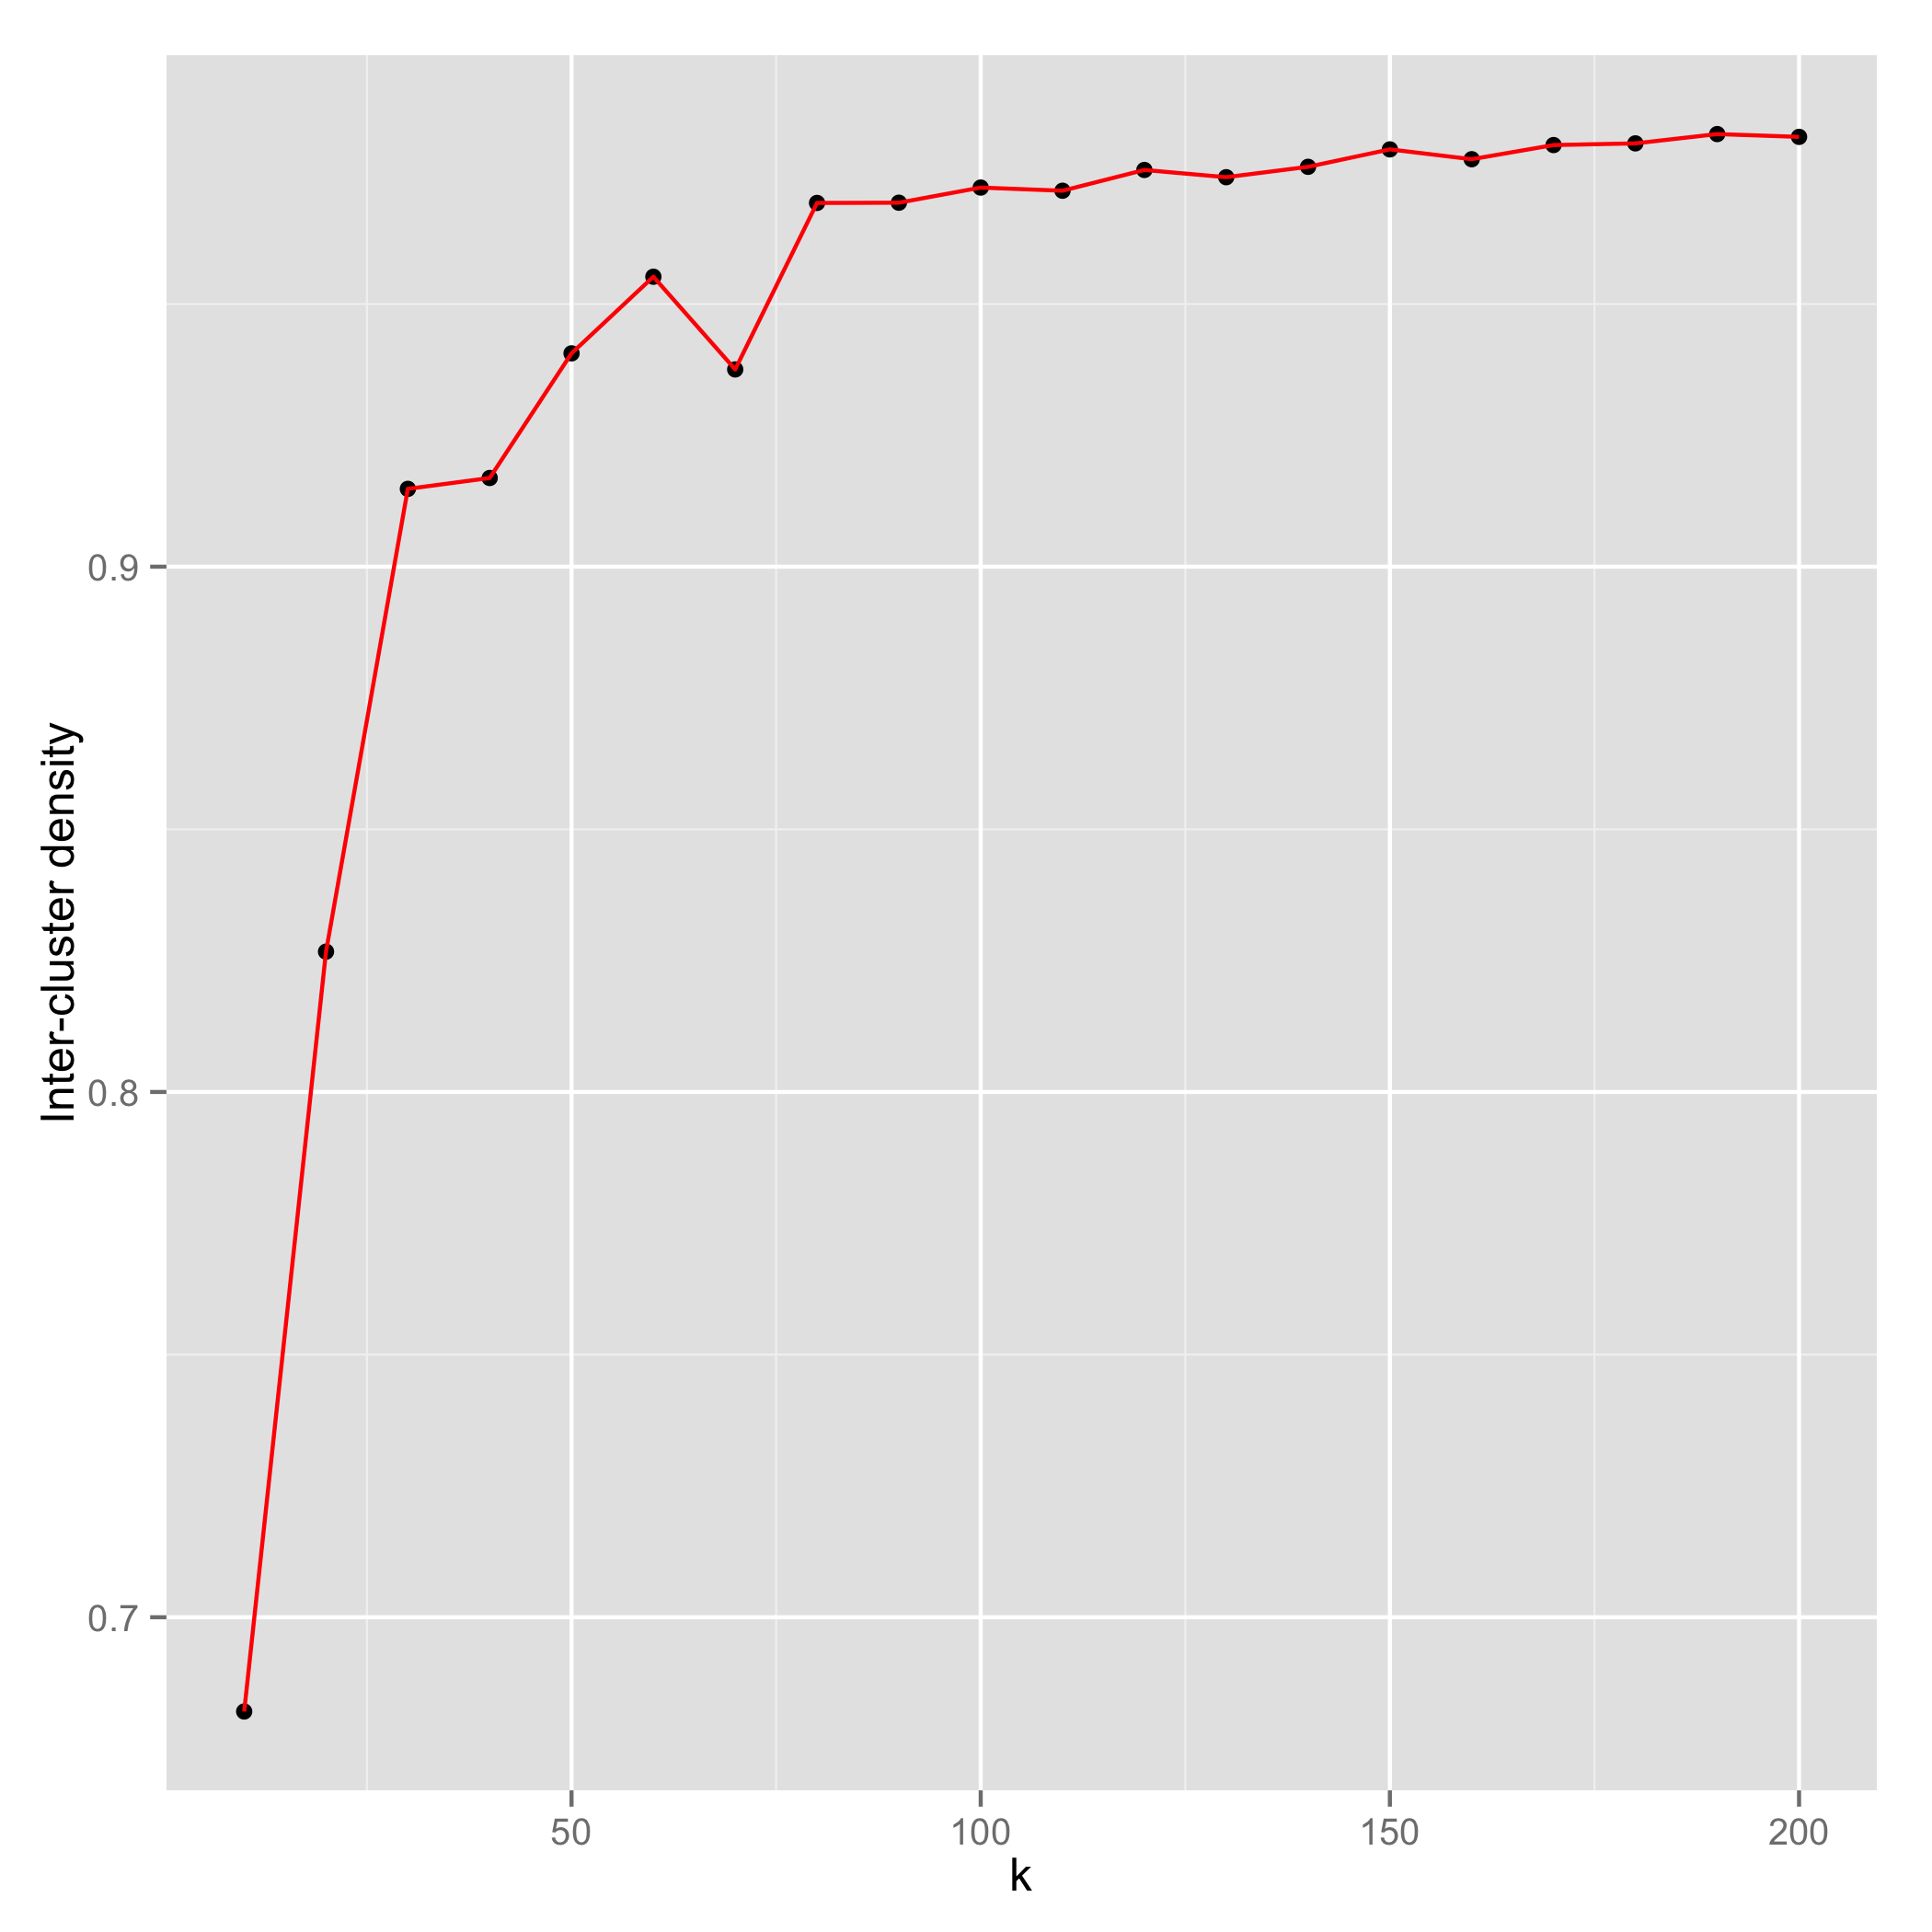
\includegraphics[width=0.7\textwidth]{lastfmelbow.png}
  \centering
  \caption{Elbow-method applied on the Last.FM data set}
  \label{fig:lastfmelbow}
\end{figure}

\autoref{fig:lastfmelbow} was created by running the spherical k-means
algorithm on the Last.FM data set repeatedly, each iteration increasing $k$ by
10 (going from 10 to 200) and measuring the inter-cluster density for each $k$.
Based on the plot in \autoref{fig:lastfmelbow} $k = 60$ seems like a good fit
for the Last.FM data set.

\subsection{Performance and running time}
There are three controllable parameters that might influence the running time of
these clustering jobs. The amount of clusters, $k$, and the cardinality and
dimensionality of the data set.

\autoref{fig:lastfmvaryk} shows the running time of clustering the Last.FM data
set using spherical k-means on a modern laptop computer. Apart from the outlier
when $k = 80$ the running time seems to depend linearly on the value of $k$.


\begin{figure}[htbp]
  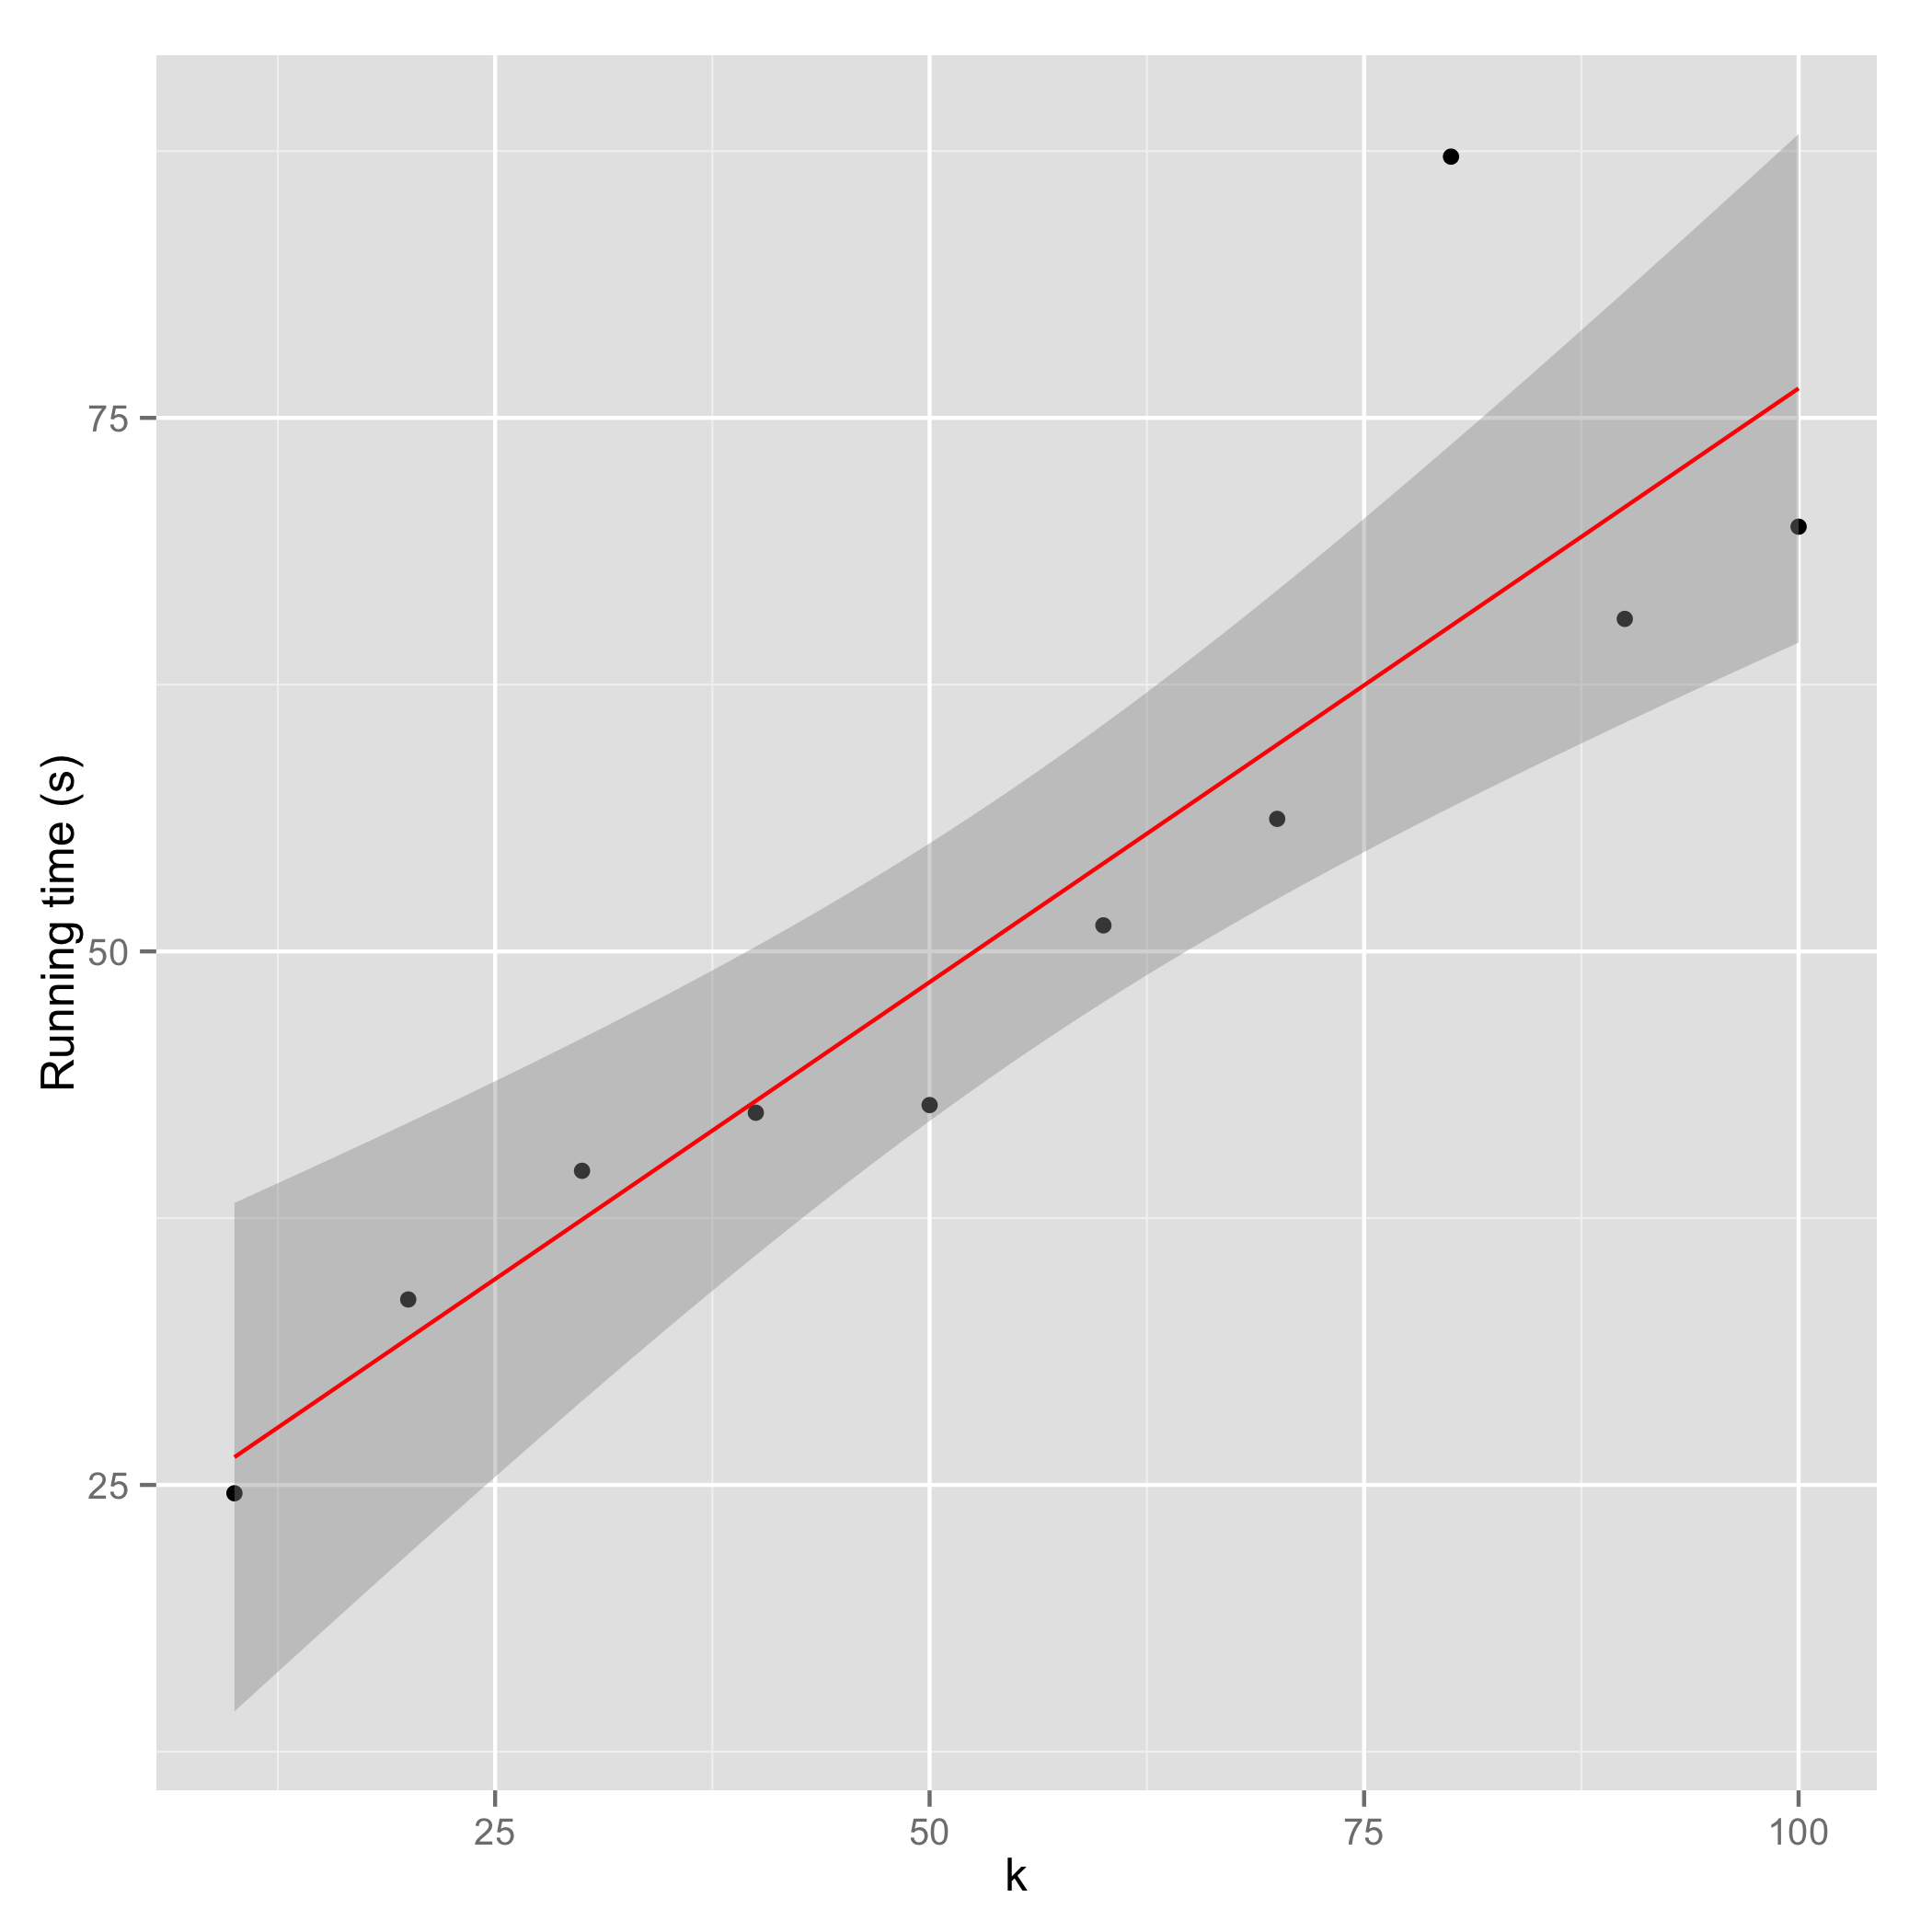
\includegraphics[width=0.7\textwidth]{lastfm_varying_k.png}
  \centering
  \caption{Running time for varying values of $k$}
  \label{fig:lastfmvaryk}
\end{figure}

\autoref{fig:lastfmvarycard} shows how removing a certain percentage of the
artists in the Last.FM data set at random influences the running time of the
clustering algorithm. The x-axis indicates the percentage of artists still in
the data set, so 100\% equals the full data set. As expected, the running time
increases as more data points are used.

\begin{figure}[htbp]
  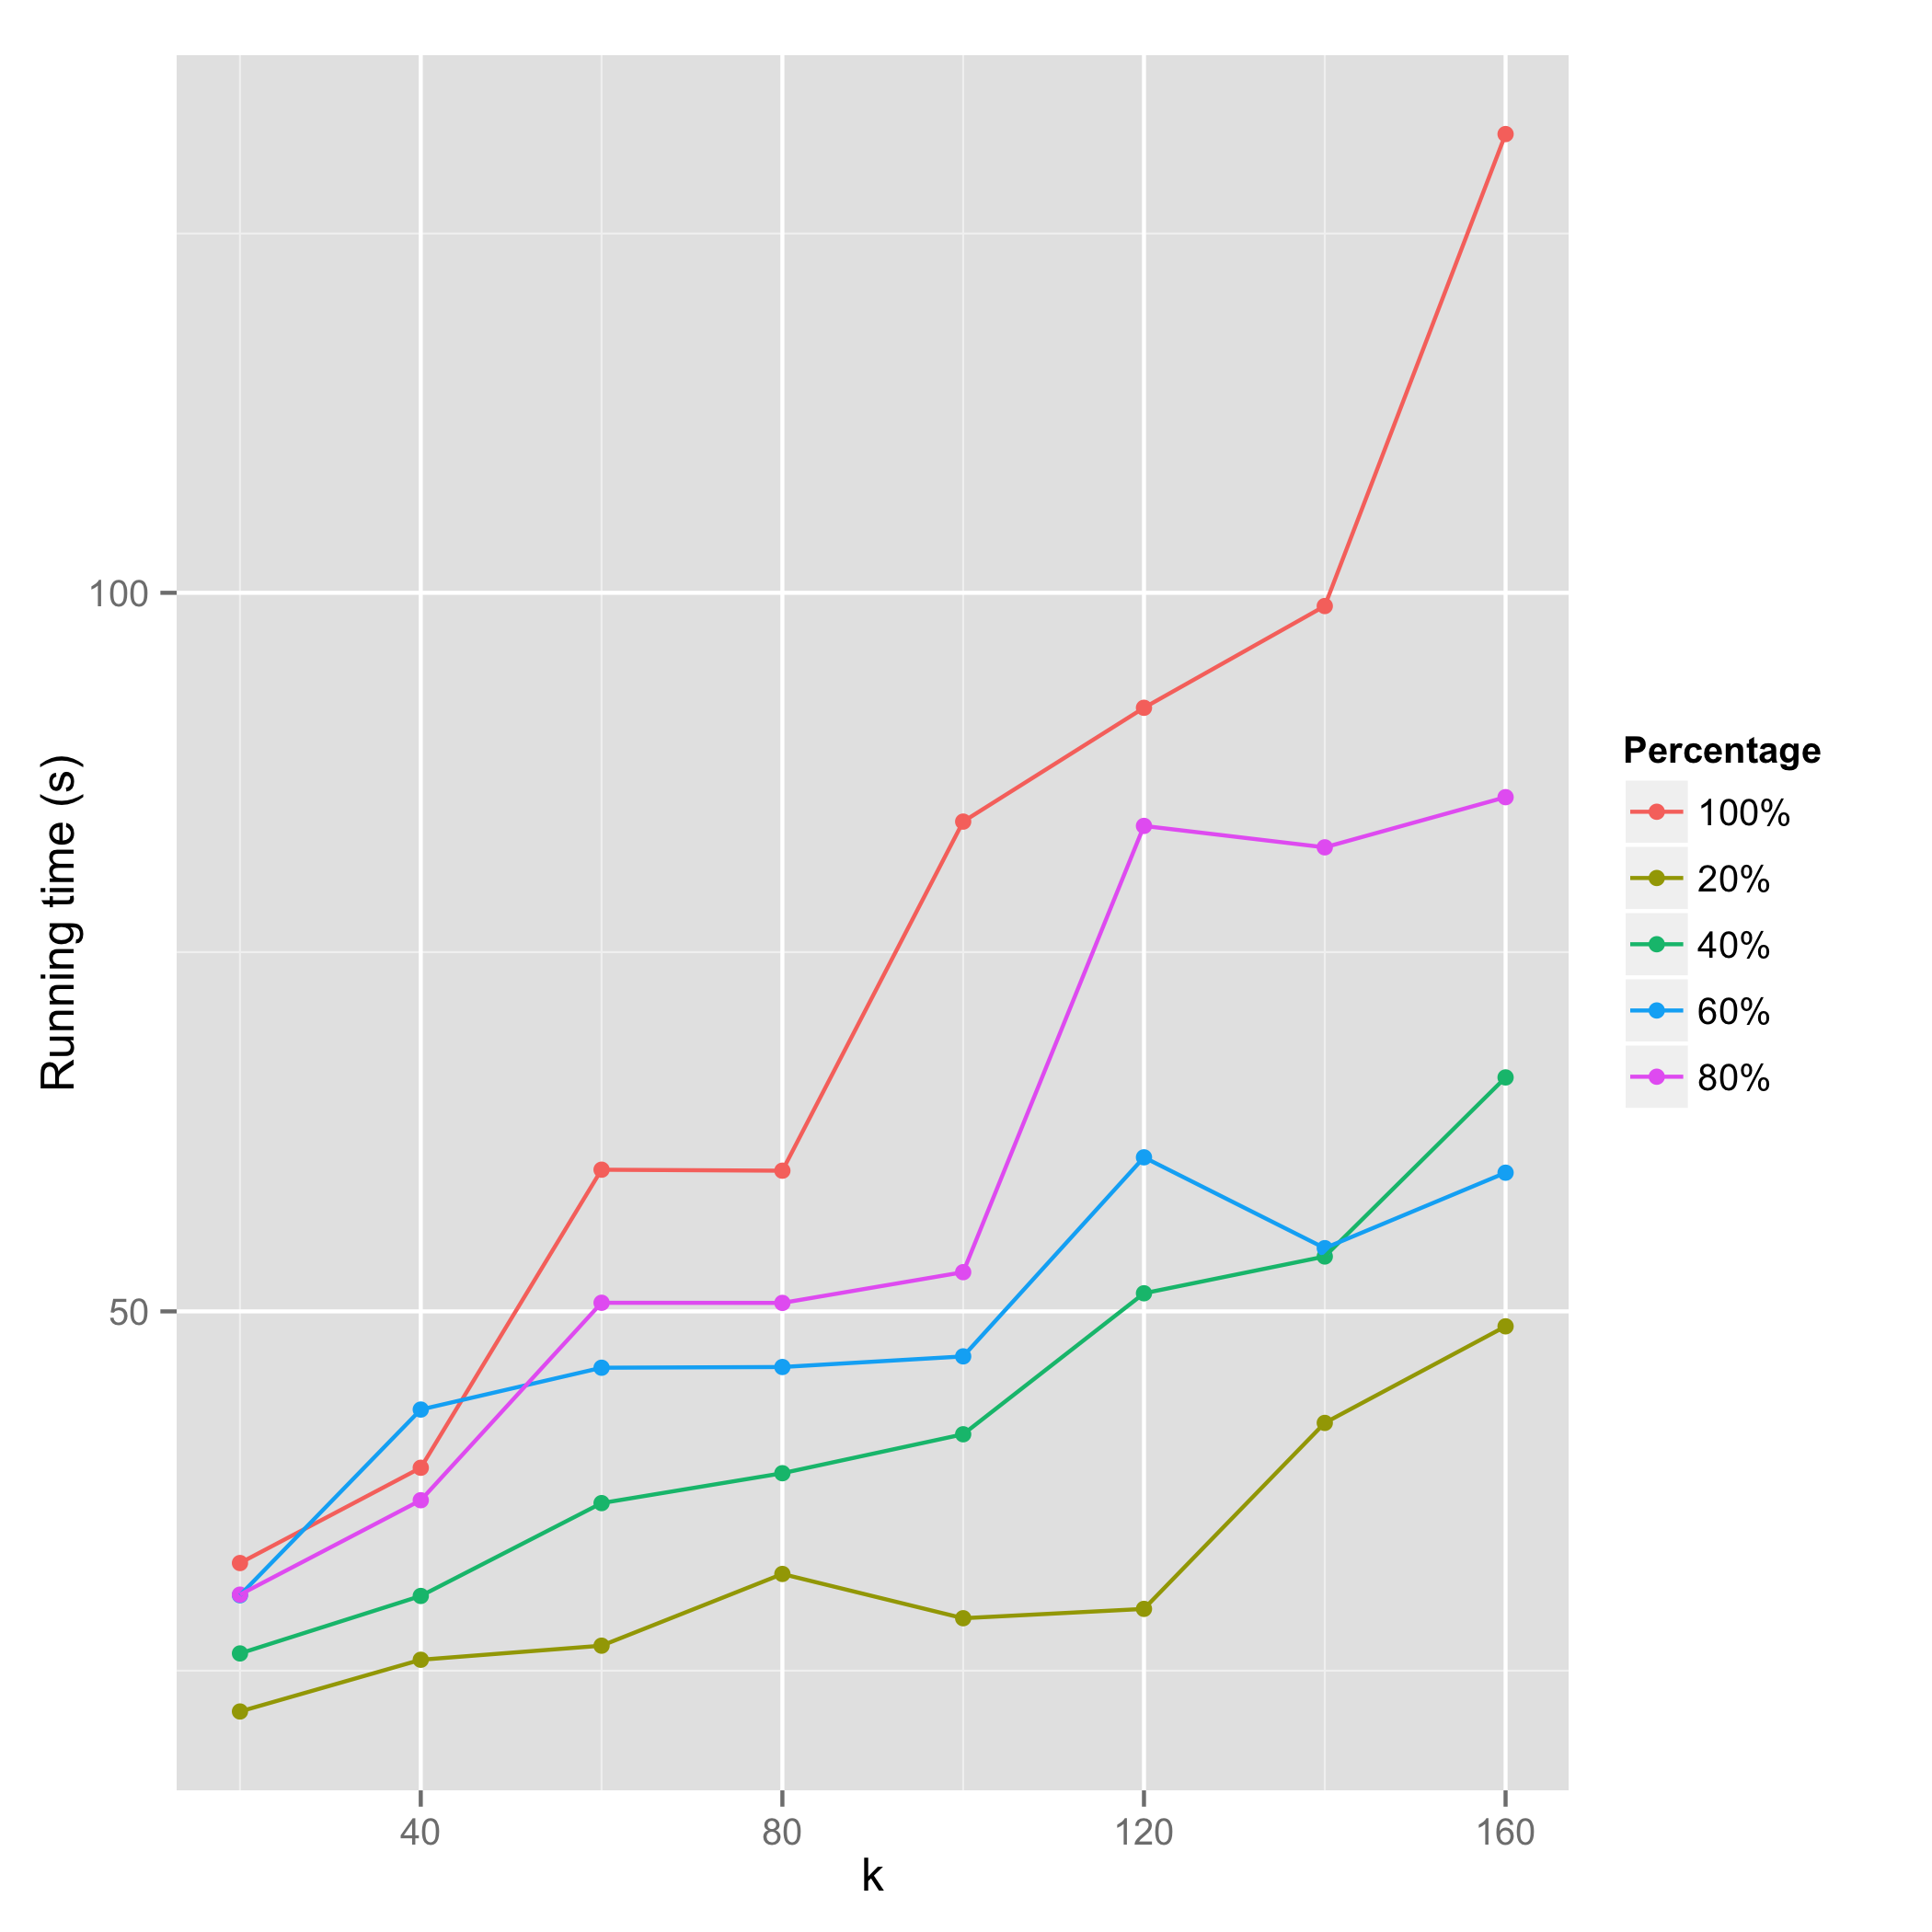
\includegraphics[width=0.7\textwidth]{lastfm_varying_card.png}
  \centering
  \caption{Running time for varying percentages of data points}
  \label{fig:lastfmvarycard}
\end{figure}

Finally, \autoref{fig:lastfmvarydim} shows how the running time changes as only
20\%, 40\%, 60\%, 80\% and 100\% of tags are used, reducing the dimensionality
in steps. The increase is not quite as distinguished between different
percentages as in \autoref{fig:lastfmvarycard}, but we can definitely see that
the slope increases when using a higher percentage of tags.

\begin{figure}[htbp]
  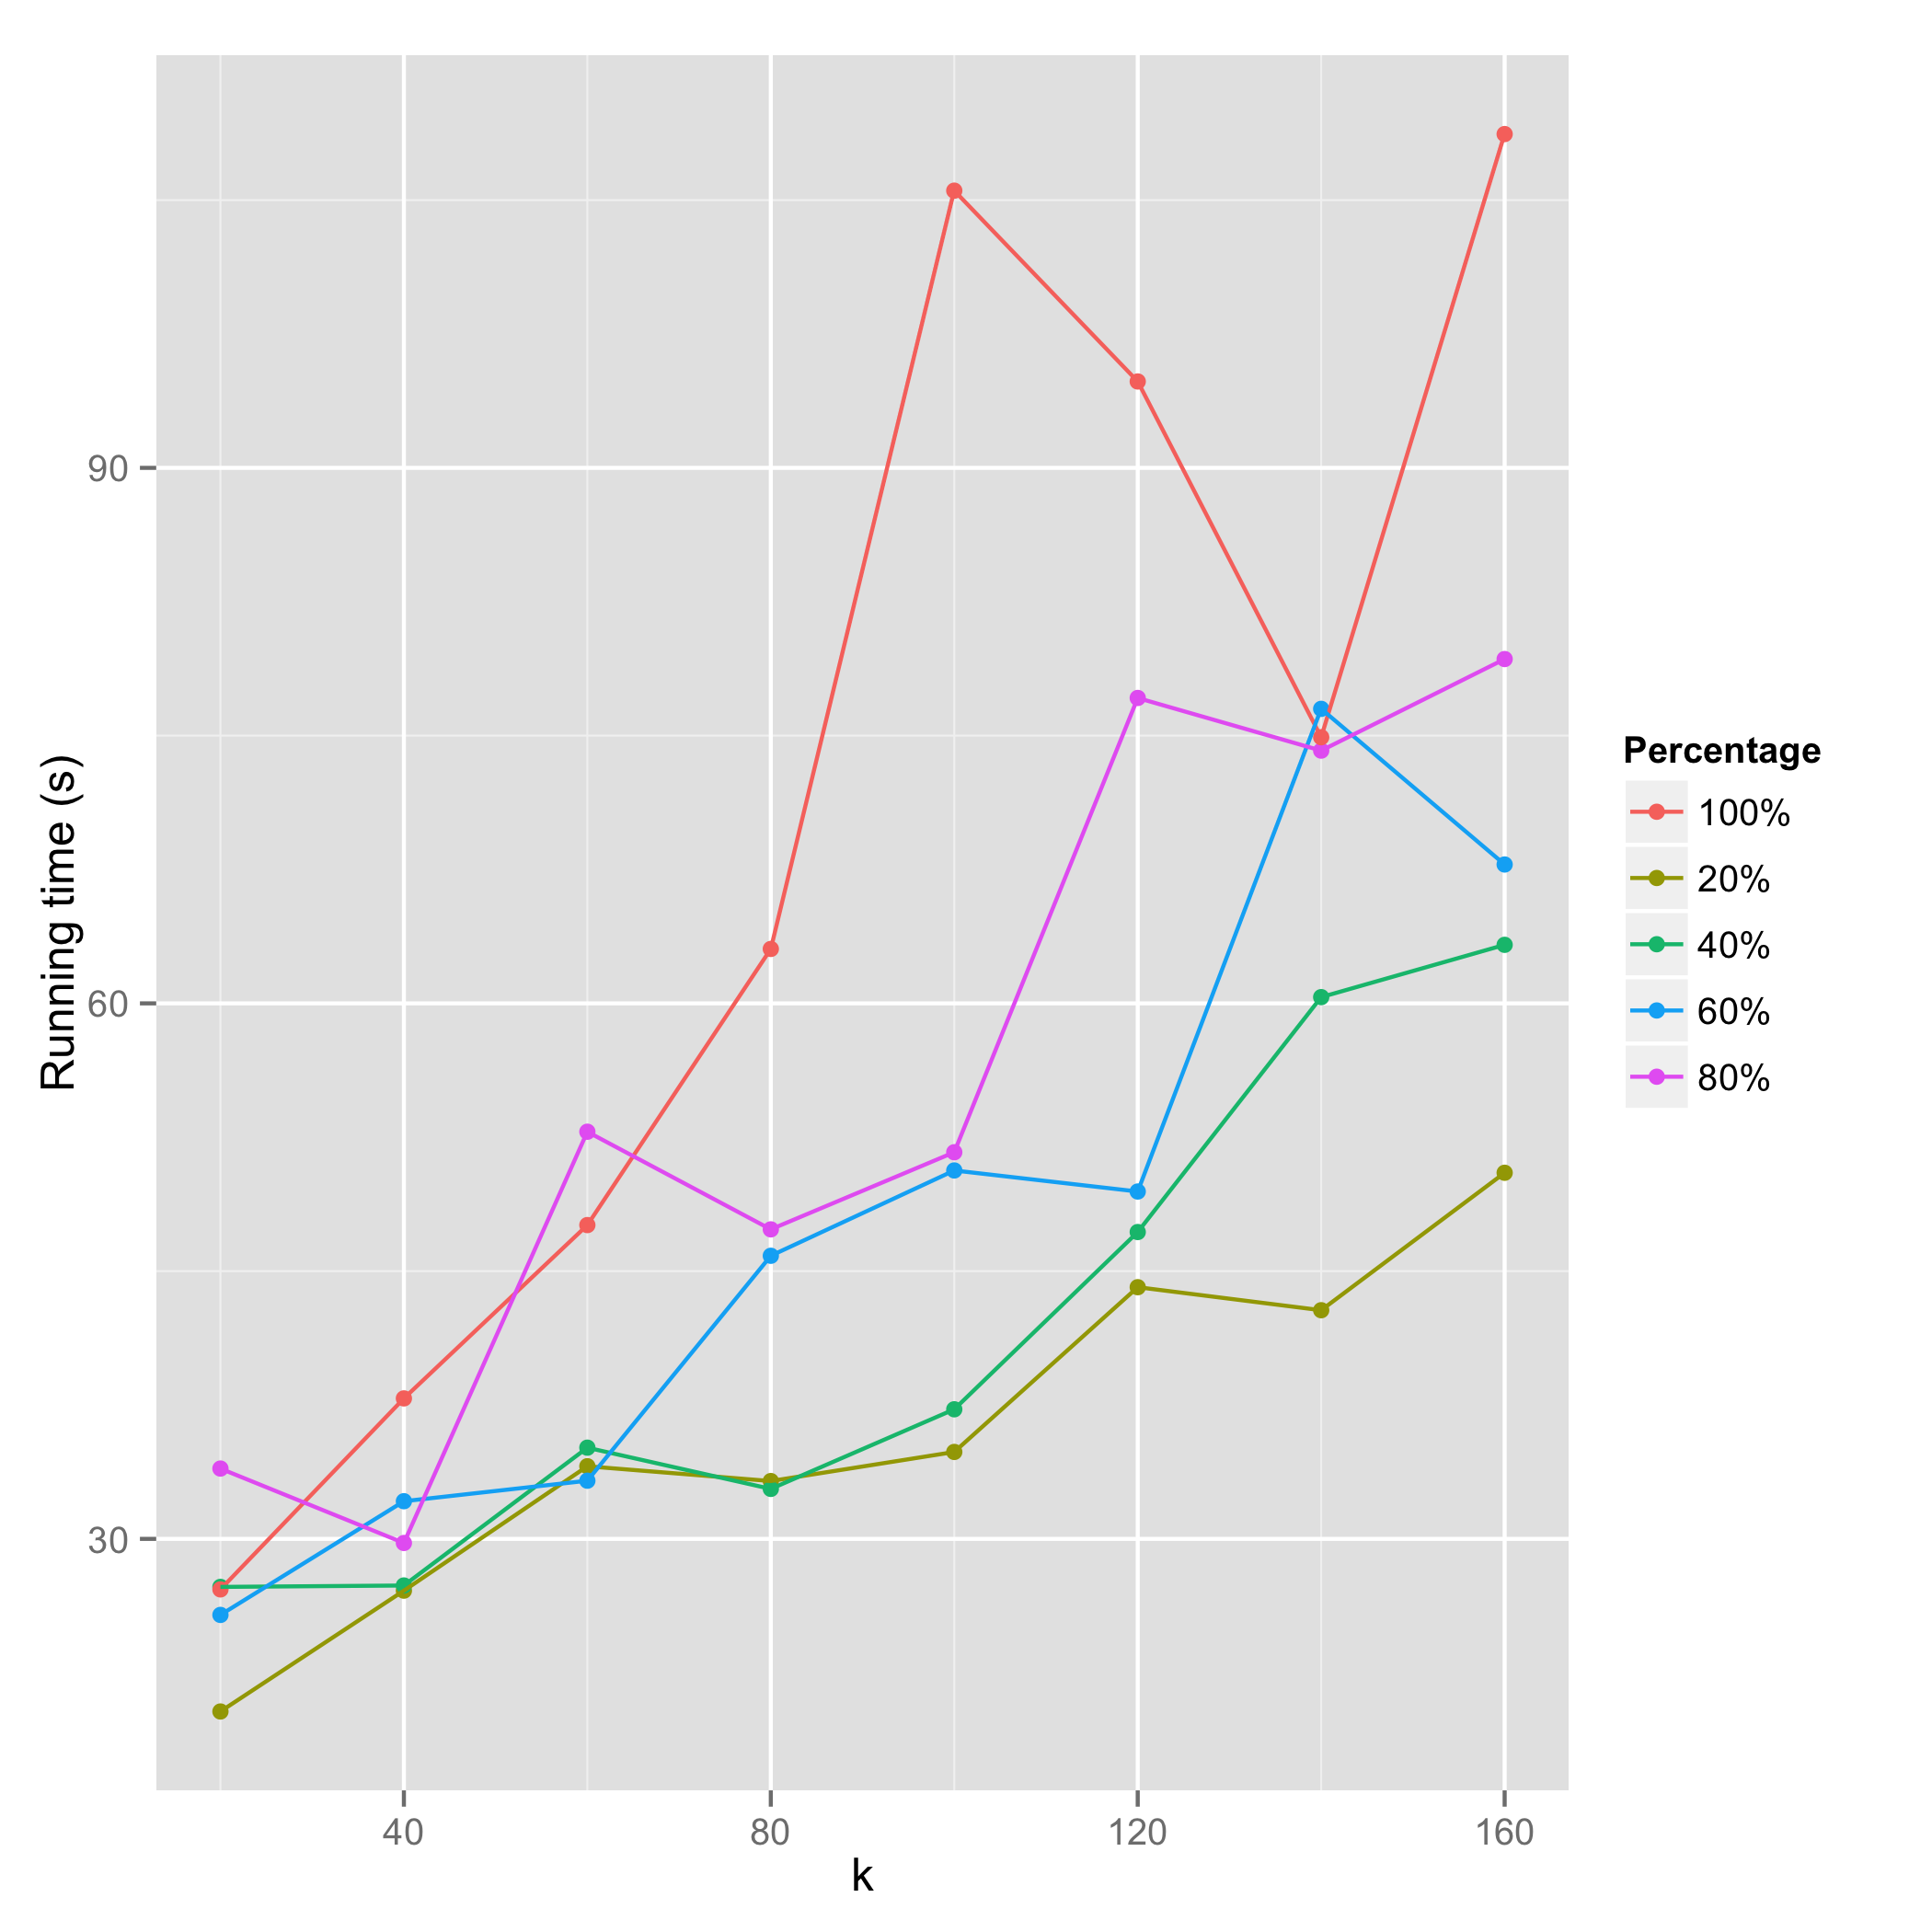
\includegraphics[width=0.7\textwidth]{lastfm_varying_dim.png}
  \centering
  \caption{Running time for varying percentages of dimensions}
  \label{fig:lastfmvarydim}
\end{figure}

\subsection{Scaling horizontally}
It has been established that the way Mahout's running time increases with
increases in $k$, cardinality and dimensionality is at least roughly linear.
Ideally, Mahout scales linearly with the amount of nodes available in the
cluster.

In order to determine how Mahout scales when scaling horizontally (adding more
nodes in contrast to increasing resource on a single node) two rounds of jobs
(for $ k = \left\{ {20, 40, 60, 80, 100, 120, 140, 160 }\right\} $ ). These jobs
were run on Amazon EMR (using instance type m1.large) in three batches with 5,
10 and 15 nodes respectively doing the computation. Execution times were
derived from the timestamps in the logfiles. 

In the small scale test the input data size and the size of the data in the
intermediate steps are smaller than the default HDFS block size on Amazon EMR
(128 MB). As a result, only one mapper process can run at a time effectively
eliminating the performance gains of having more nodes. For this reason, the
block size is forced to 128 KB in the tests on Amazon EMR. This will impact
performance negatively as HDFS is not optimized to read many small files, but it
will allow us to see the effect of adding more nodes (and as a result, more map
processes) on the running time. Due to this and the fact that the hardware on
Amazon EMR differs from the laptop previous test jobs were run, EMR job
performance and the performance of the jobs run on the laptop can not be
compared in a useful way. These tests are purely to see whether the running time
decreases linearly with the number of nodes in use.

\autoref{fig:emrruntimes} shows the results of this experiment. Apart from an
outlier when $k = 80$ and using 15 nodes the running times drop and the line
gets ``flatter'' as we increase the amount of nodes, indicating that the
difference in running time between the hadoop cluster configurations would
increase as $k$ increased even more, and that for this size of data set and
range of $k$ we are able to scale horizontally.

\begin{figure}[htbp]
  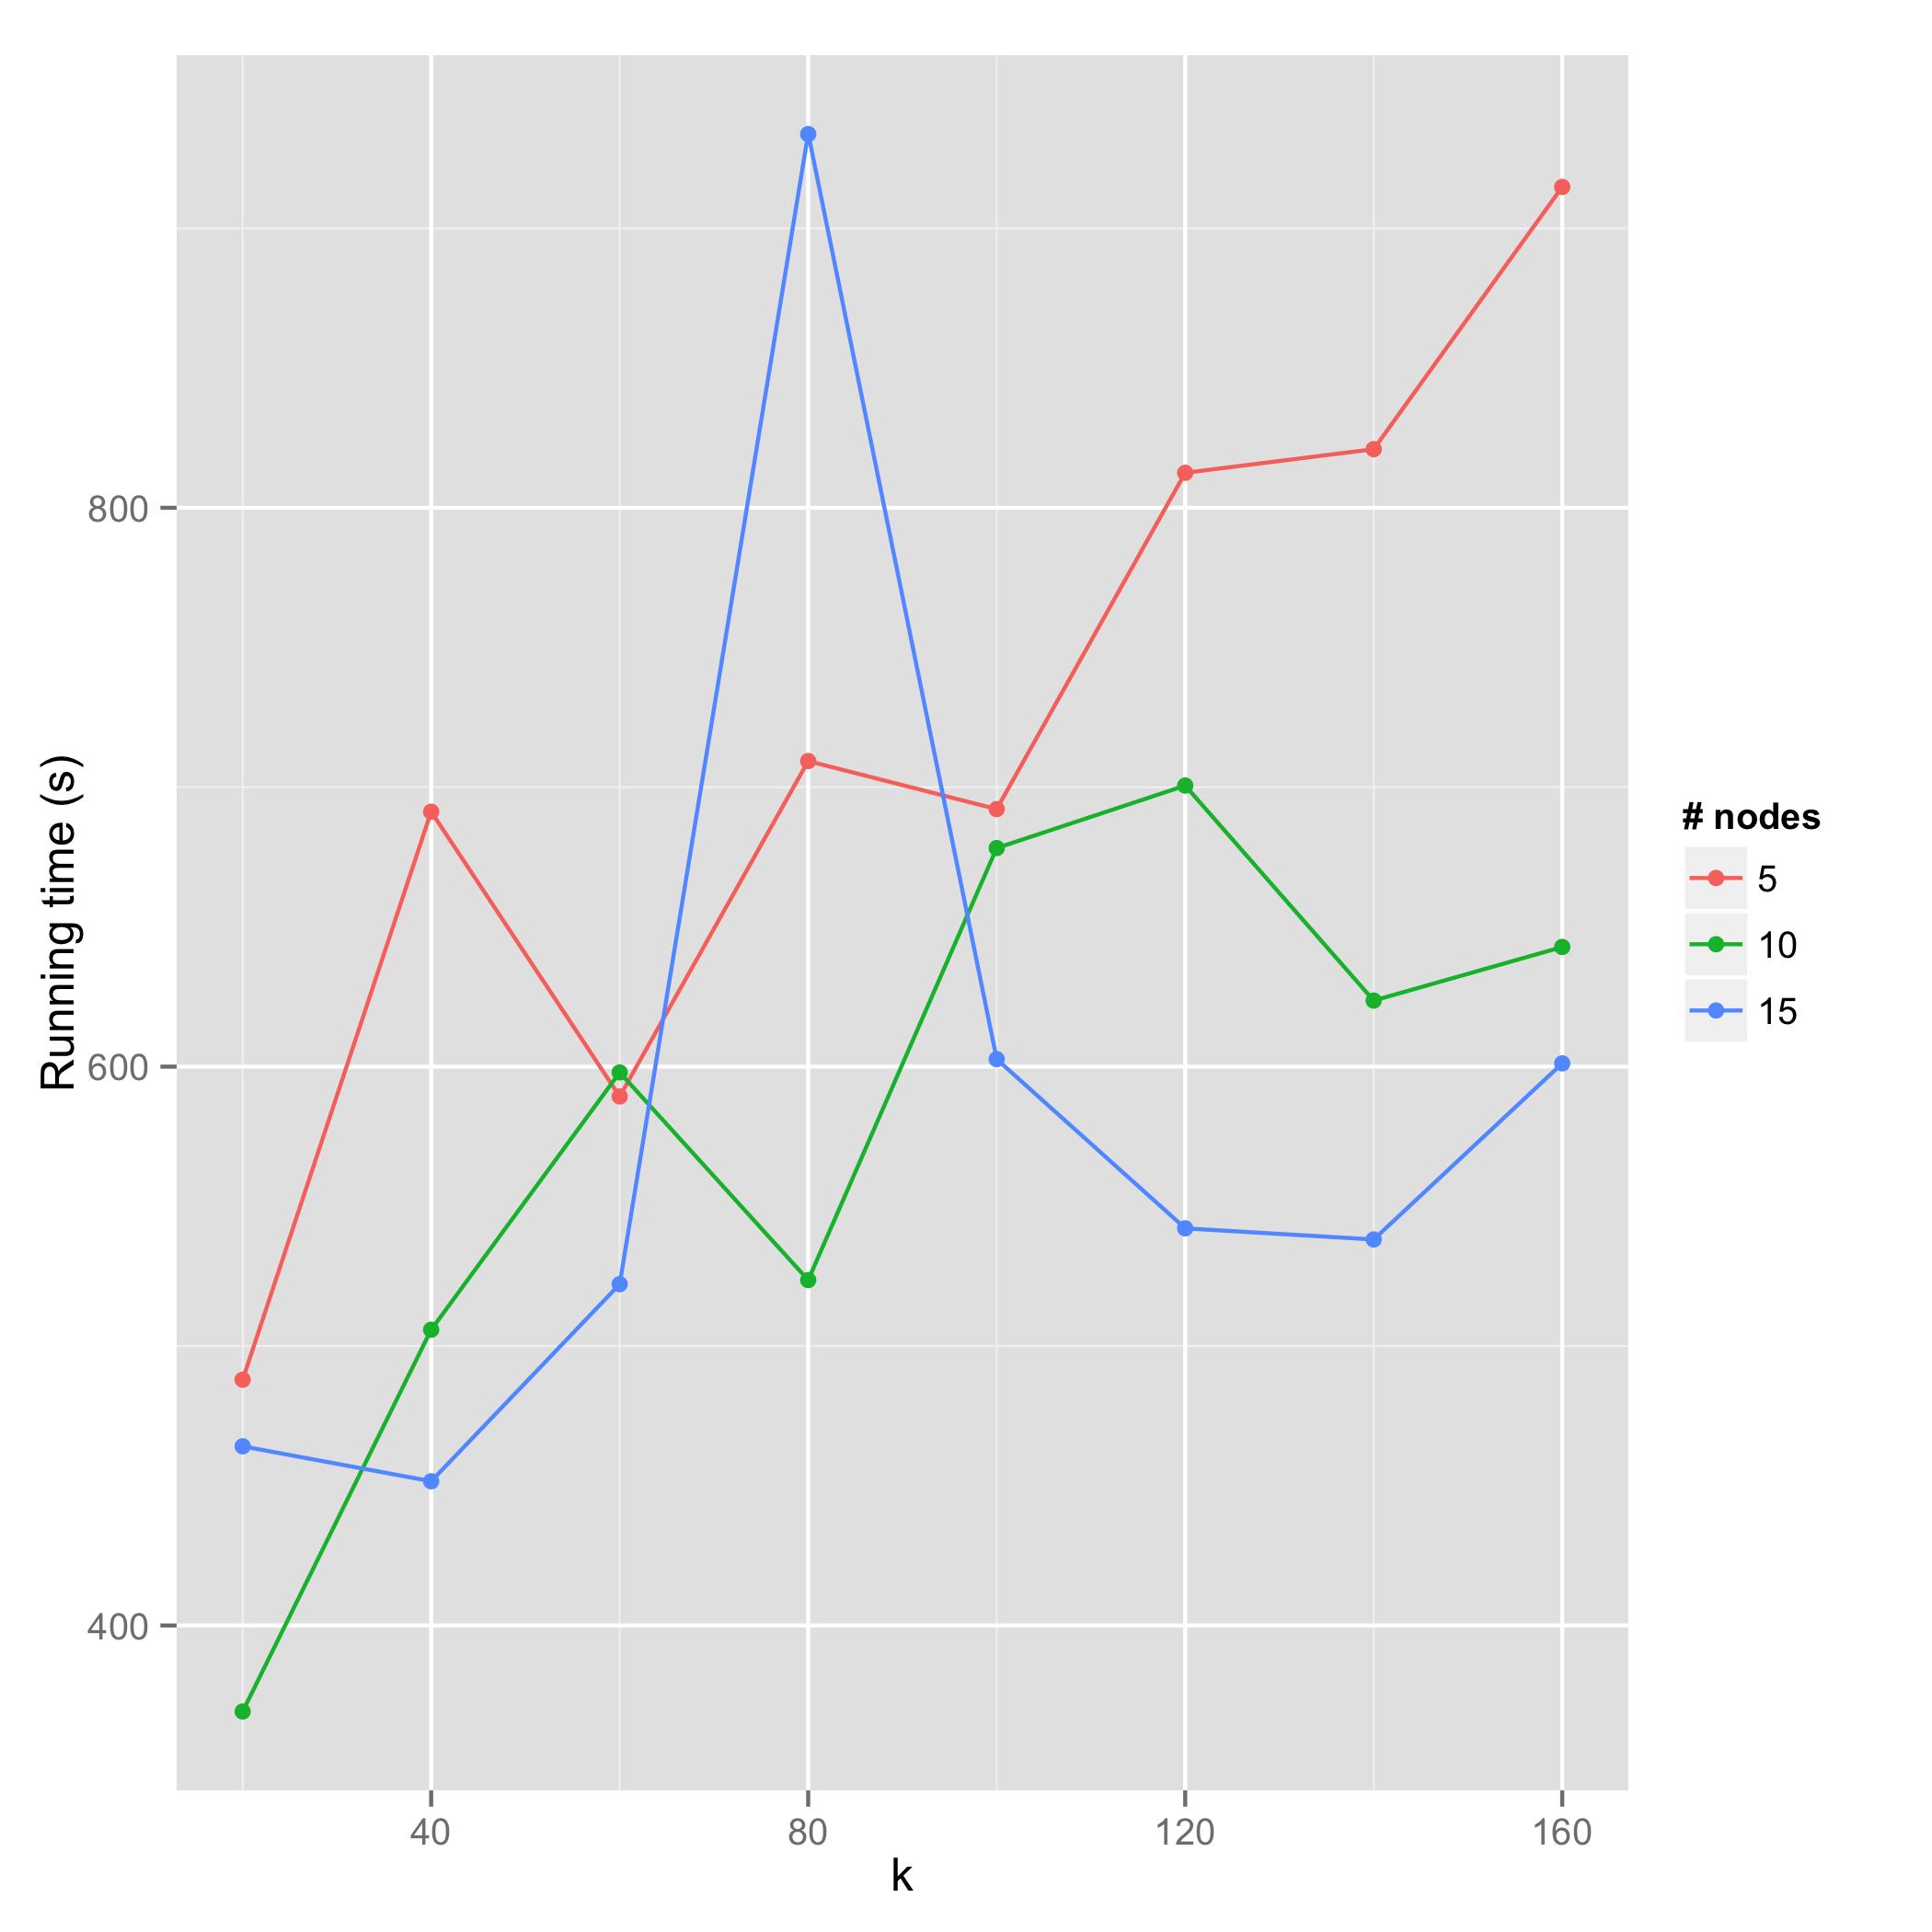
\includegraphics[width=0.7\textwidth]{running_times_emr.png}
  \centering
  \caption{Running time for different $k$ using 5, 10 and 15 nodes}
  \label{fig:emrruntimes}
\end{figure}

\subsection{Final clustering}
In the previous sections we found that $k = 60$ is a reasonable choice for the
small scale data set. In this section we present the result of such a
clustering, and use the Mahout clusterdump utility to inspect the outcome.

The easiest and most straightforward way of assessing the clustering outcome is
to visually inspect it. This is also a rather unscientific method since music
and music genres are highly subjective. Keeping this in mind, we should however
be able to spot instances where an artist defintiely does not seem to belong to
the cluster it has been assigned to and get at least a subjective ``feel'' for
the quality of the clustering. \autoref{tbl:lastfmkmeans} shows a few non-random
artists and the top tags in the cluster they belong to. The artists were chosen
solely on the basis of being well-known enough that any reader should be able to
determine whether they fit in their cluster or not.

\begin{table}
\centering
  \begin{tabular}{ |l|l|l| }
  \hline
  Artist name & Top tags in cluster & Weight of tag \\
  \hline
  \multirow{4}{*}{The Rolling Stones} & classic rock & 0.192 \\
   & hard rock & 0.160 \\
   & hair metal & 0.092 \\
   & rock & 0.073 \\

  \hline

  \multirow{4}{*}{Bob Dylan} & singer-songwriter & 0.152 \\
   & folk & 0.094 \\
   & acoustic & 0.075 \\
   & female vocalists & 0.065 \\

  \hline

  \multirow{4}{*}{Madonna} & 80s & 0.163 \\
   & new wave & 0.138 \\
   & post-punk & 0.087 \\
   & pop & 0.083 \\

  \hline

  \multirow{4}{*}{Frank Sinatra} & jazz & 0.346 \\
   & lounge & 0.082 \\
   & acid jazz & 0.080 \\
   & downtempo & 0.067 \\

  \hline

  \multirow{4}{*}{Antonio Vivaldi} & Classical & 0.762 \\
   & piano & 0.140 \\
   & contemporary classical & 0.120 \\
   & opera & 0.106 \\

  \hline

  \multirow{4}{*}{Eminem} & Hip-Hop & 0.294 \\
   & rap & 0.233 \\
   & hip hop & 0.188 \\
   & hiphop & 0.070 \\

  \hline

  \end{tabular}
  \caption{Results of K-means clustering of the Last.FM data set}
  \label{tbl:lastfmkmeans}
\end{table}

Overall, these six artists look like they have been assigned to sane clusters.
Madonna would probably not be considered ``post-punk'' by most people but
``80s'' and ``pop'' certainly fits in my opinion. Artists tagged with
``post-punk'' might also often be tagged with ``80s''. The same situation
applies to Bob Dylan and ``female vocalists''.

It is also interesting to see whether or not artists considered as close (in a
musical sense) have ended up in the same clusters. Again, I will use the artists
from \autoref{tbl:lastfmkmeans} and choose six additional artists that
\textit{I} believe should be in the same cluster. As before, this is a
subjective test of the clustering quality, which of course is a subjective
quality in its own. 

\begin{table}
\centering
  \begin{tabular}{ |l|l|l| }
  \hline
  Artist \#1 & Artist \#2 & Same cluster? \\
  \hline
  The Rolling Stones & The Who & Yes \\
  Bob Dylan & Neil Young & Yes \\
  Madonna & Kylie Minogue & No \\  
  Frank Sinatra & Dean Martin & Yes \\
  Antonio Vivaldi & Ludwig van Beethoven & Yes \\
  Eminem & 2Pac & Yes \\
  \hline
  \end{tabular}
  \caption{Comparing cluster assignment of similar artists}
  \label{tbl:lastfmcompare}
\end{table}

Looking at the results in \autoref{tbl:lastfmcompare}, most of the artists fall
into the same, expected cluster. The one miss is Kylie Minogue who did not end
up in the same cluster as Madonna. This could be due to the subjective nature of
my choice or the fact that the ``australian'' tag is very common for Kylie
Minogue but obviously not for Madonna. All in all, for this very small subset of
the artists the clustering seems to agree with my perception of which artists
should share a cluster. The full output of centroids can be found in appendix
\ref{app:lastfmkmeans}.

There are some quantative features of the clustering that can be examined as
well. For instance, we can compare the various sizes of the clusters. In this
case, we see that the mean size of the clusters is 347.72 data points per
cluster, the largest having 1141 data points and the smallest only a single
data point. The standard deviation is quite high, 245.81, indicating that the
sizes of the clusters vary quite heavily, as also indicated by the difference
in the maximum and minimum cluster sizes.

Finally, as discussed before, at $k = 60$ the rate of increase in inter-cluster
density flattens out which is why $k = 60$ was chosen in the first place. For
this particular clustering output the inter-cluster density is 0.9244, again
showing fairly evenly distributed clusters. The intra-cluster density, i.e. the
average distance between the data points within a cluster, is 0.734. This is a
bit higher than I suspected, but since it is quite a bit lower than the 
inter-cluster density it still seems like the clusters are nicely separated.


\section{Spherical K-Means with Canopy seeding}
As mentioned in the survey, using Canopy clustering to see the k-means
clustering can give both faster convergence as well as produce more accurate
results. I will therefore extend our previous experiment with spherical k-means
to be seeded by a canopy clustering.

The authors of \cite{mccallum2000} report better results in practice when using
different distance metrics for the canopy clustering and the second stage
clustering (Spherical K-Means in the current context). For this reason, the
cosine similarity will not be used for the canopy clustering step. Instead, I
tried using the Tanimoto distance. The reasoning behind the choice being that
since the Tanimoto distance is smaller for vectors that have components in
common and hopefully this leads to initial centroids that are close to other
vectors with common components. The reasoning was that it would work well with
the cosine similarity since the cosine similarity depends on vector components
that are both non-zero.

Unfortunately, due to the sparsity and high-dimensionality of the data this
turned out to be a dead end. The $T_1$ and $T_2$ thresholds had to be very large
because of the sparsity and dimensionality. Previously, we have established
$k = 60$ to be a good choice for $k$, but even with $T_2 = 0.999$ canopy
clustering still yielded 70-80 clusters to be used as initial centroids. In
general, seeding k-means clustering with the output from canopy clustering can
be very useful, but it also needs a way of estimating good values for $T_1$ and
$T_2$. Usually, this is done by someone knowledgable in the field based on the
dimensions applicable. In this case, this is not possible due to the very high
dimensional nature of the data. Since canopy clustering is rather fast, $T_1$
and $T_2$ could be estimated by running the clustering several times to find
what values for $T_1$ and $T_2$ would give the sought for number of
canopies.\cite[p.~158]{owen2011mahout} This is the approach taken here, but I
still could not find suitable values to produce the number of clusters I was
looking for.

\section{Latent Dirichlet Allocation}
With k-means, each document was assigned to a single cluster, where the cluster
is defined by a centroid vector in the vector space.  With LDA, each document is
instead assigned a set of probabilities, each giving the probability of a word
in the document coming from a corresponding topic. As mentioned, Mahout
implements Latent Dirichlet Allocation using Collapsed Variational Bayes to
infer the latent topics.\cite{mahoutlda} 

\subsection{Performance and running time}
Much like for k-means we will investigate how three parameters affect the
performance of the LDA clustering algorithm in Mahout. These are the choice of
number of topics and the dimensionality and cardinality of the data set. There
are other parameters like smoothing for the document-topic and topic-term
distributions, but in this project these have been kept constant at the Mahout
default, 0.0001.  For all these tests, unless otherwise specified, 5\% of the
data was held for perplexity testing and the tests were run each iteration until
the change was less than 0.05. The running of the perplexity test will affect
the running time negatively, but since it was consistently run for all tests the
effect should be constant.

\autoref{fig:lda-running-times} shows how the algorithm running time differs
when increasing the amount of topics sought for. A rather clear linear
relationship can be seen.

\begin{figure}[htbp]
  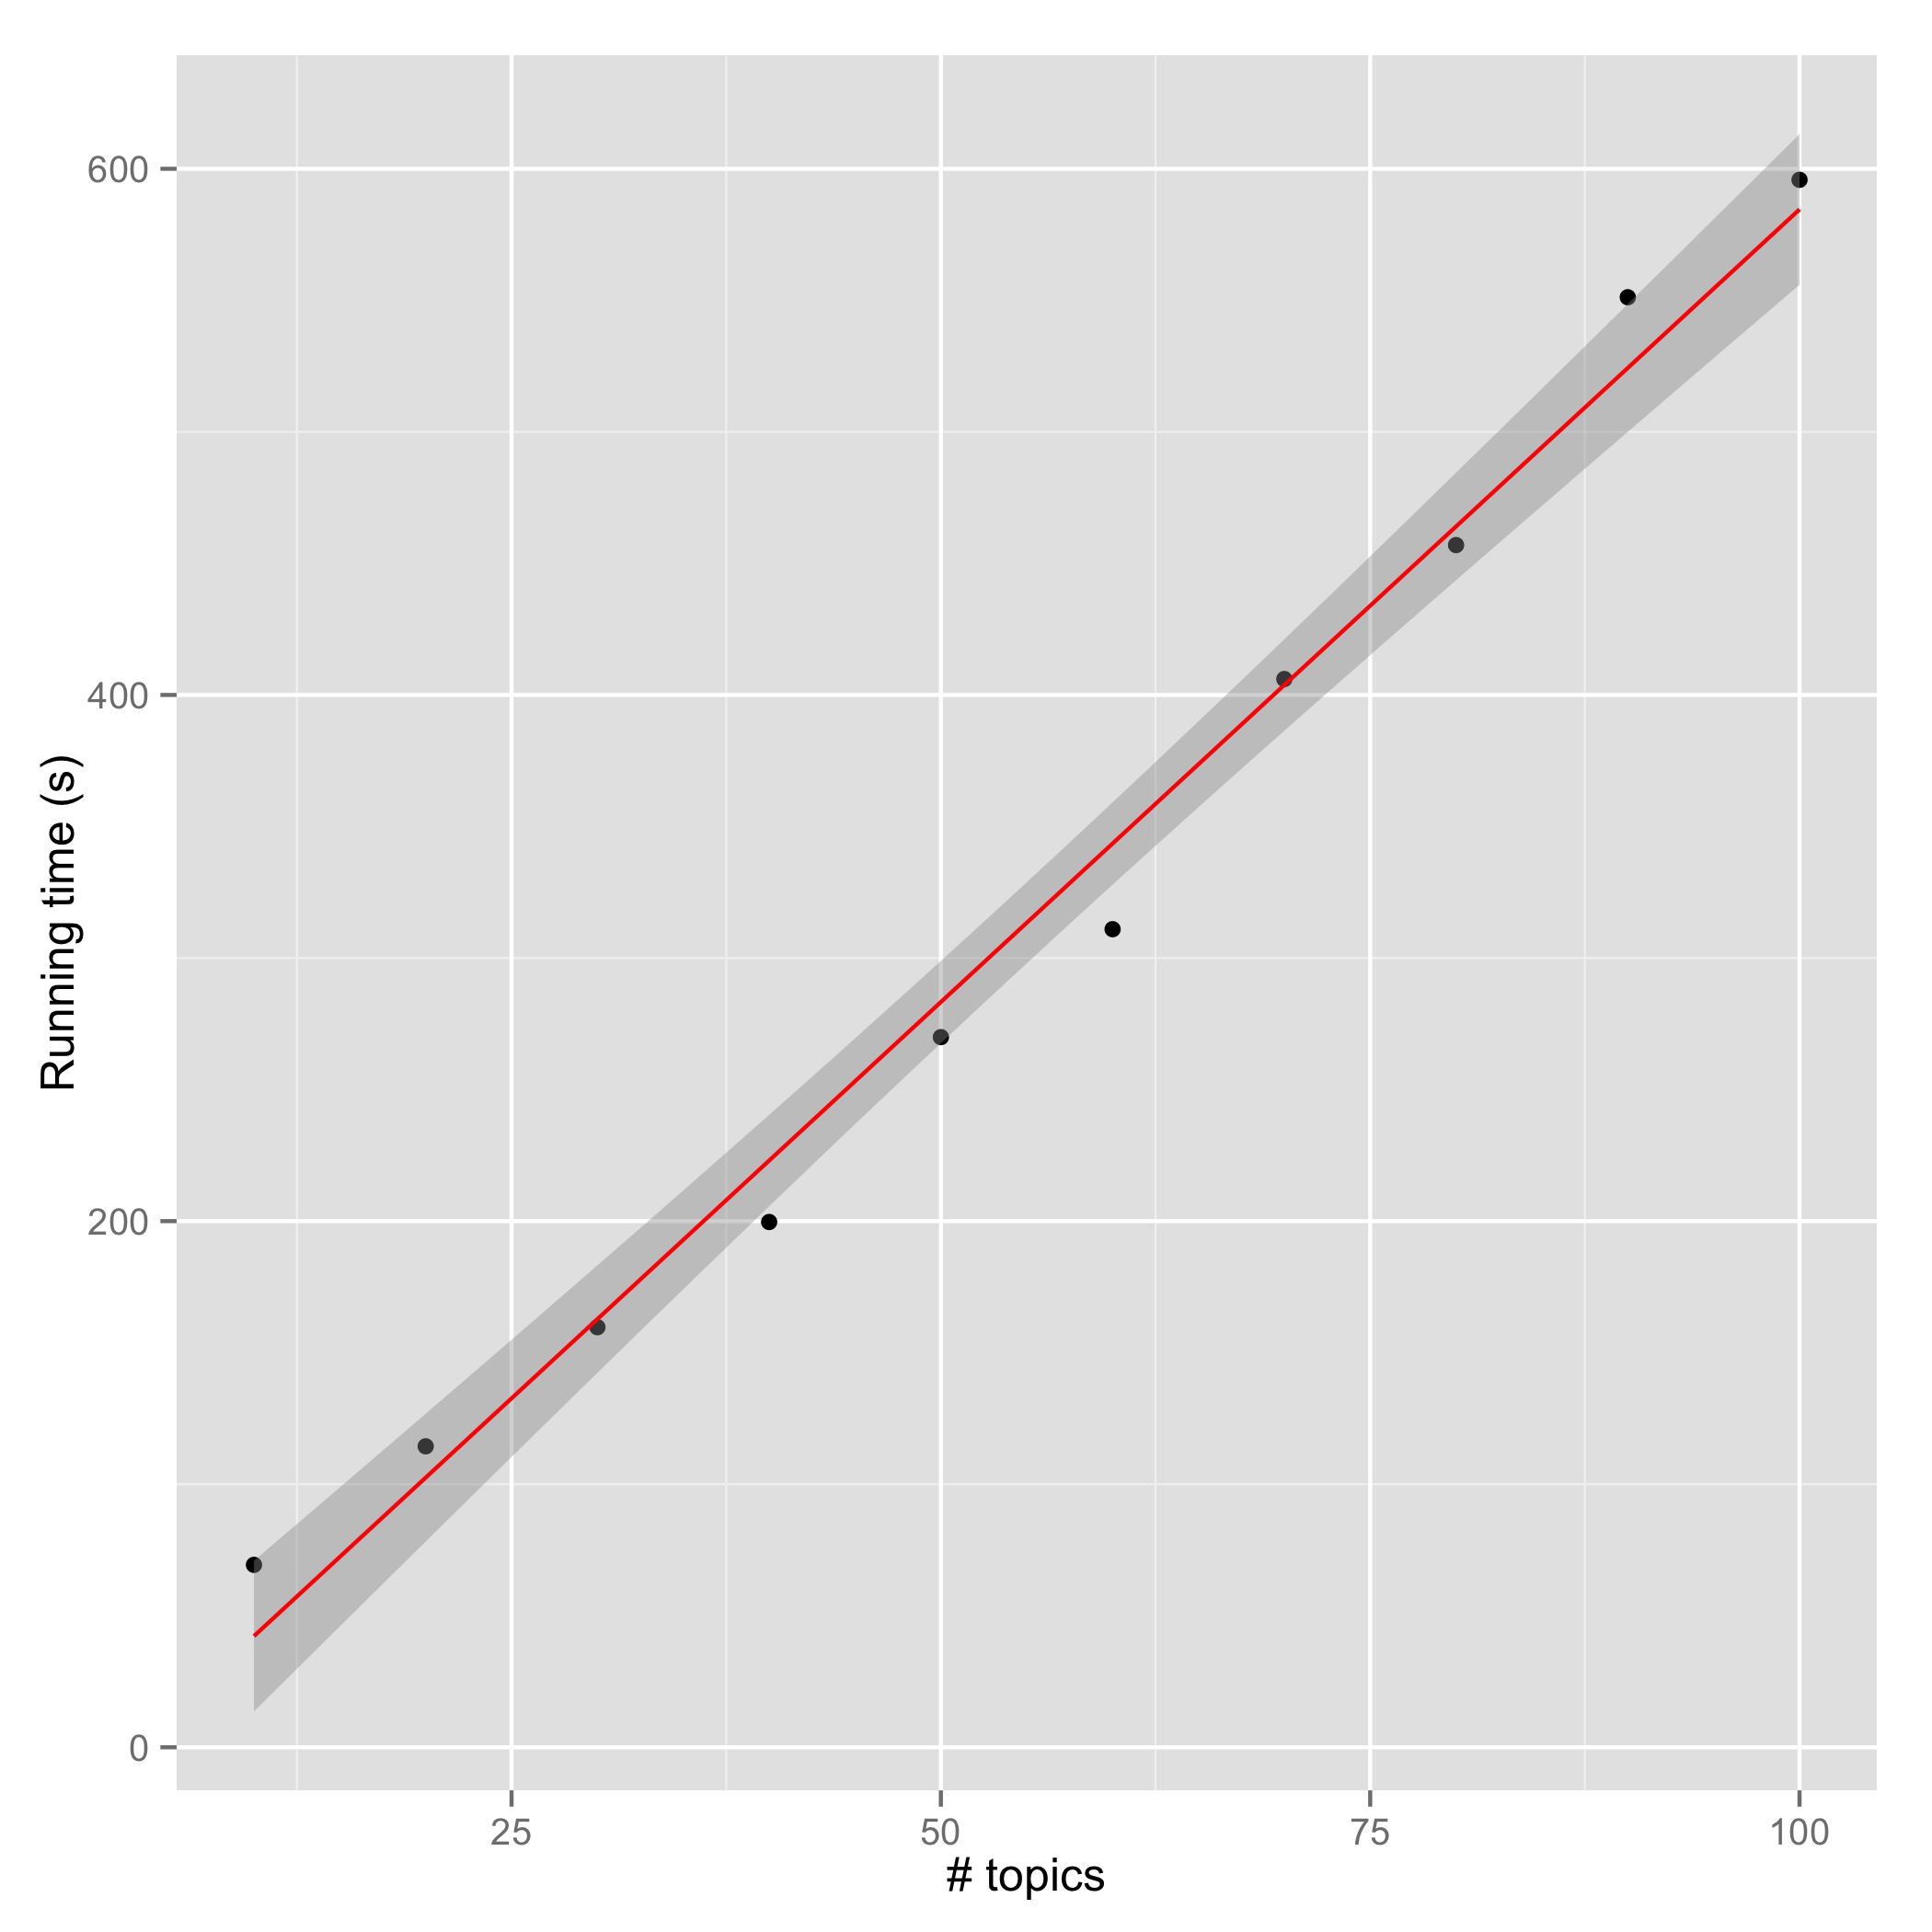
\includegraphics[width=0.7\textwidth]{lda_running_times.png}
  \centering
  \caption{Running time for different amount of topics}
  \label{fig:lda-running-times}
\end{figure}

\autoref{fig:lda-card} shows how the running time of the algorithm depends on
the cardinality of the data set. As was the case with k-means, the slope
decreases as the percentage of data points used decreases. There is however an
increase starting at $k = 80$ that does not quite follow the linear pattern seen
for $k < 80$.

\begin{figure}[htbp]
  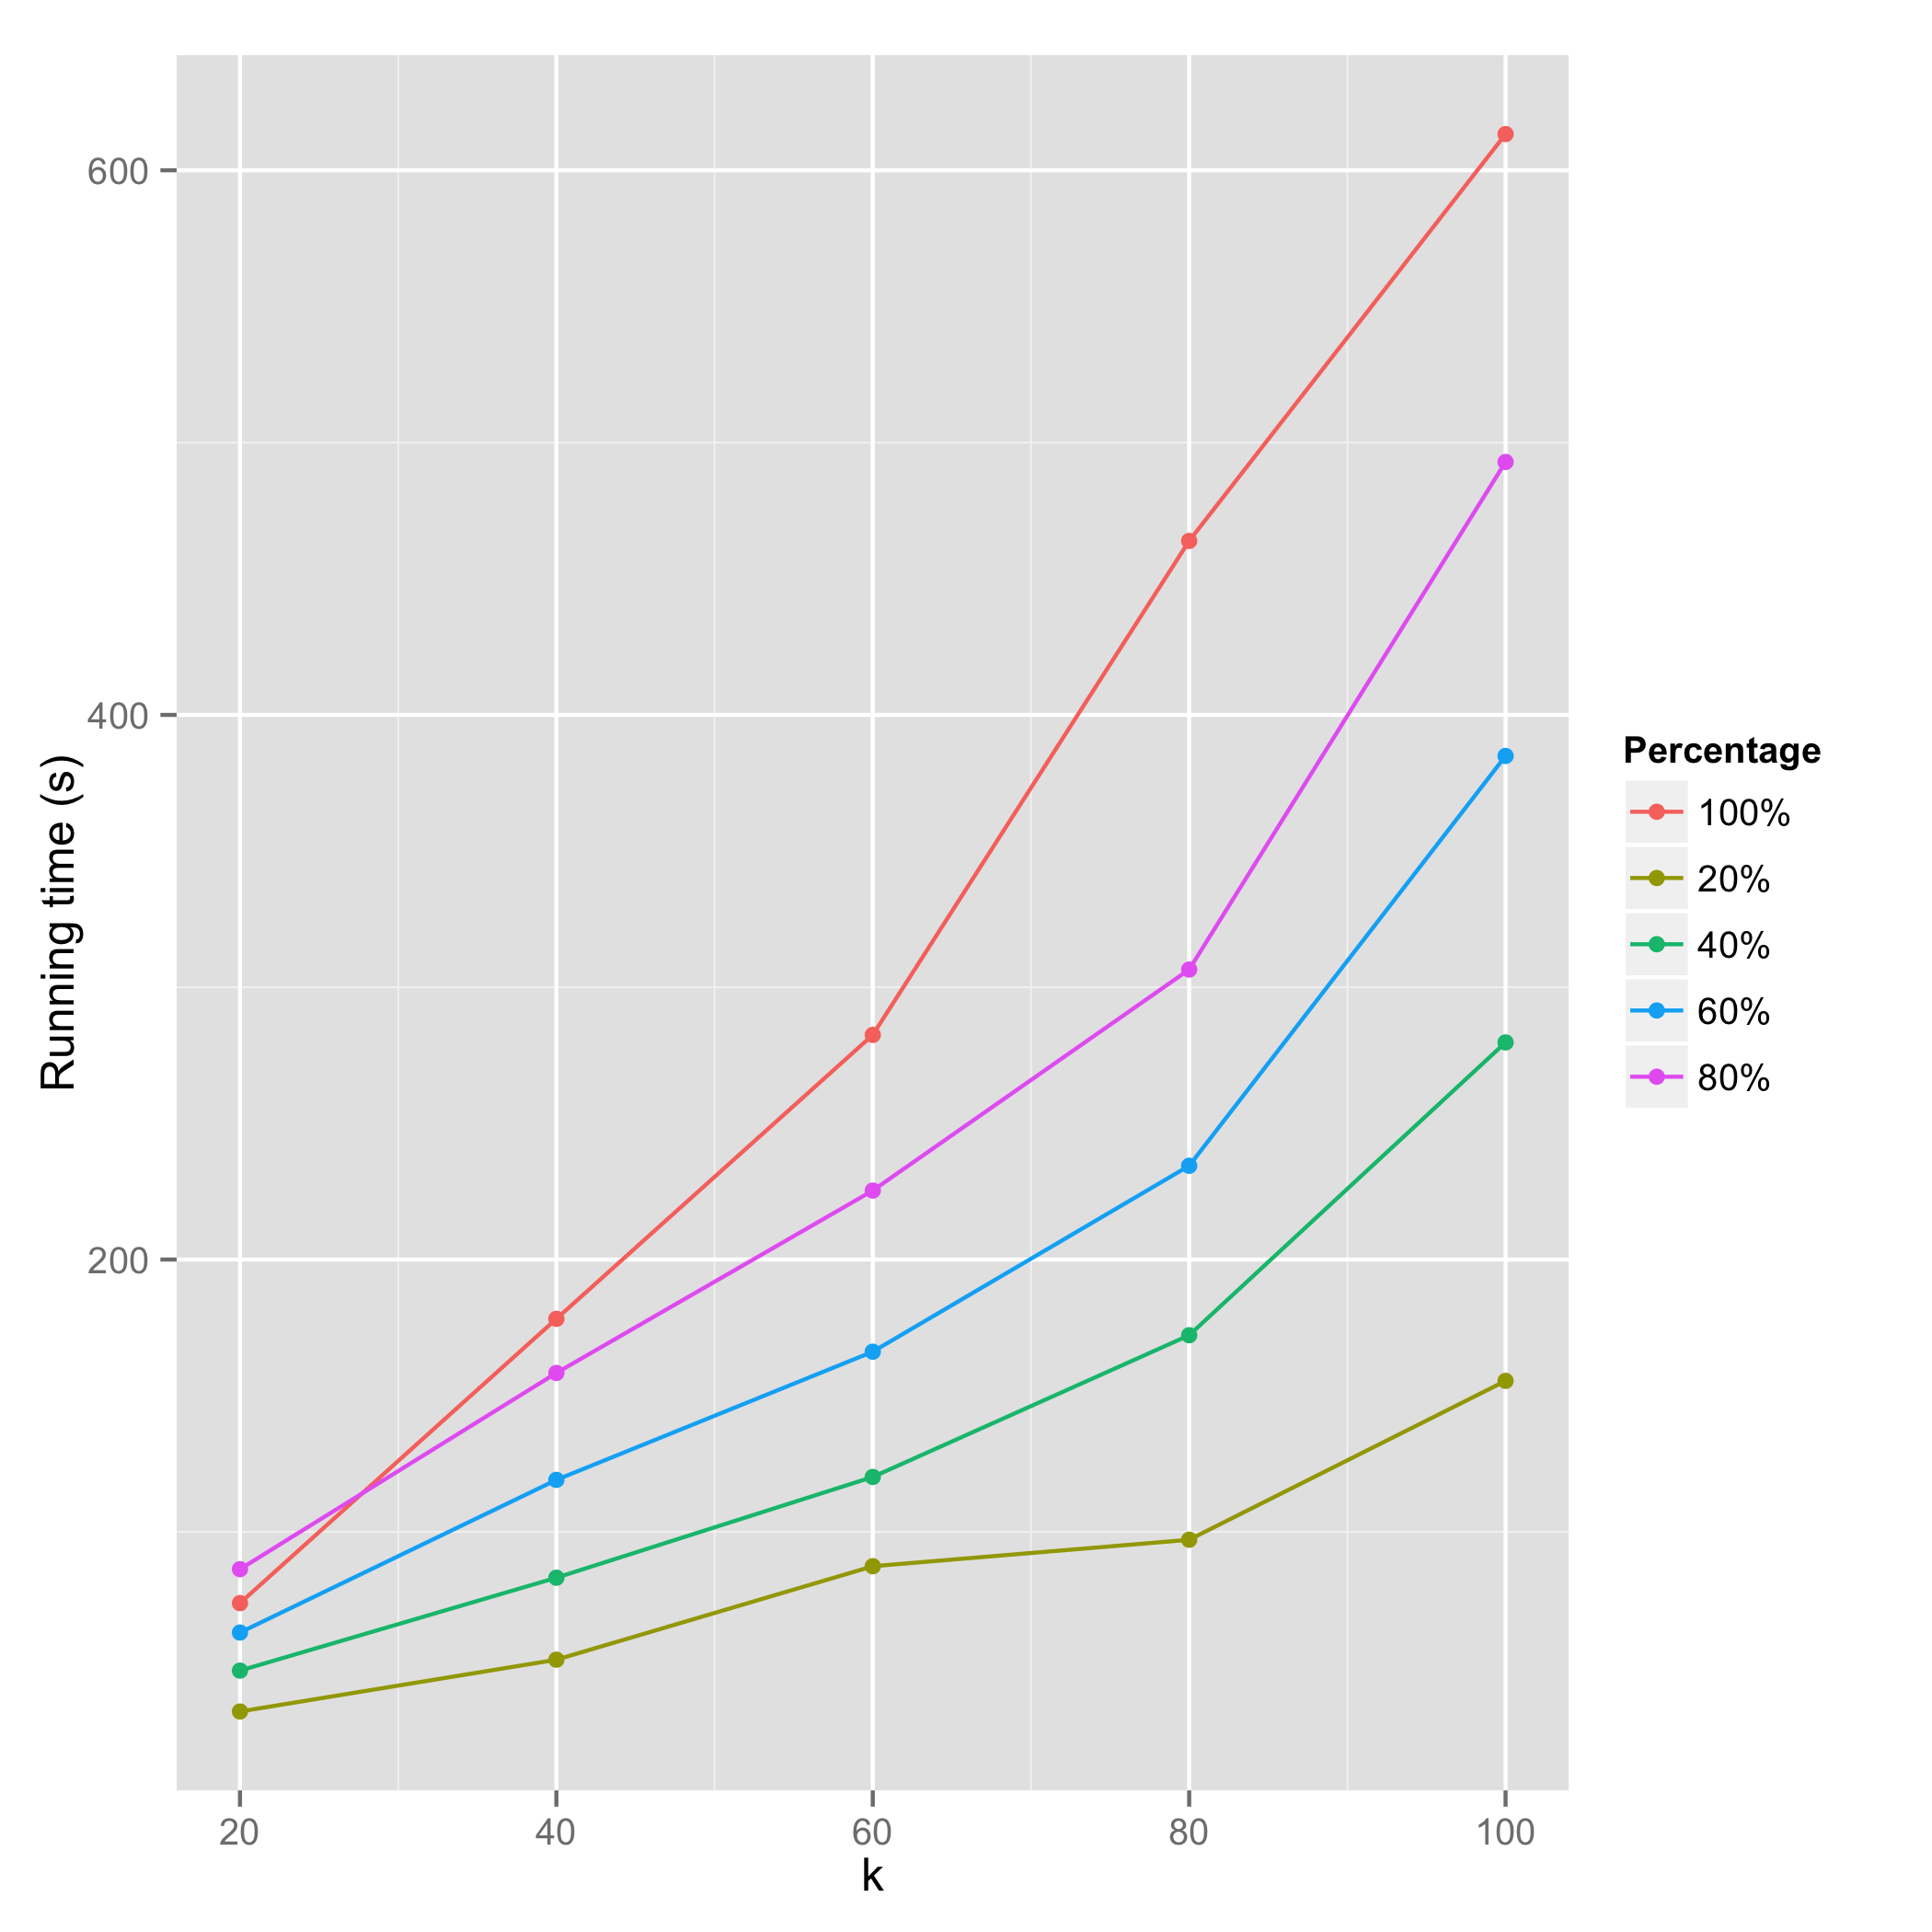
\includegraphics[width=0.7\textwidth]{lda_card.png}
  \centering
  \caption{Running time for various percentages of data points}
  \label{fig:lda-card}
\end{figure}

\autoref{fig:lda-dim} shows the result of the same procedure, but instead of
reducing the cardinality of the data set the dimensionality has been reduced.
Again, a relationship between running time and the percentages as seen in
\autoref{fig:lda-card} can be seen here too.

\begin{figure}[htbp]
  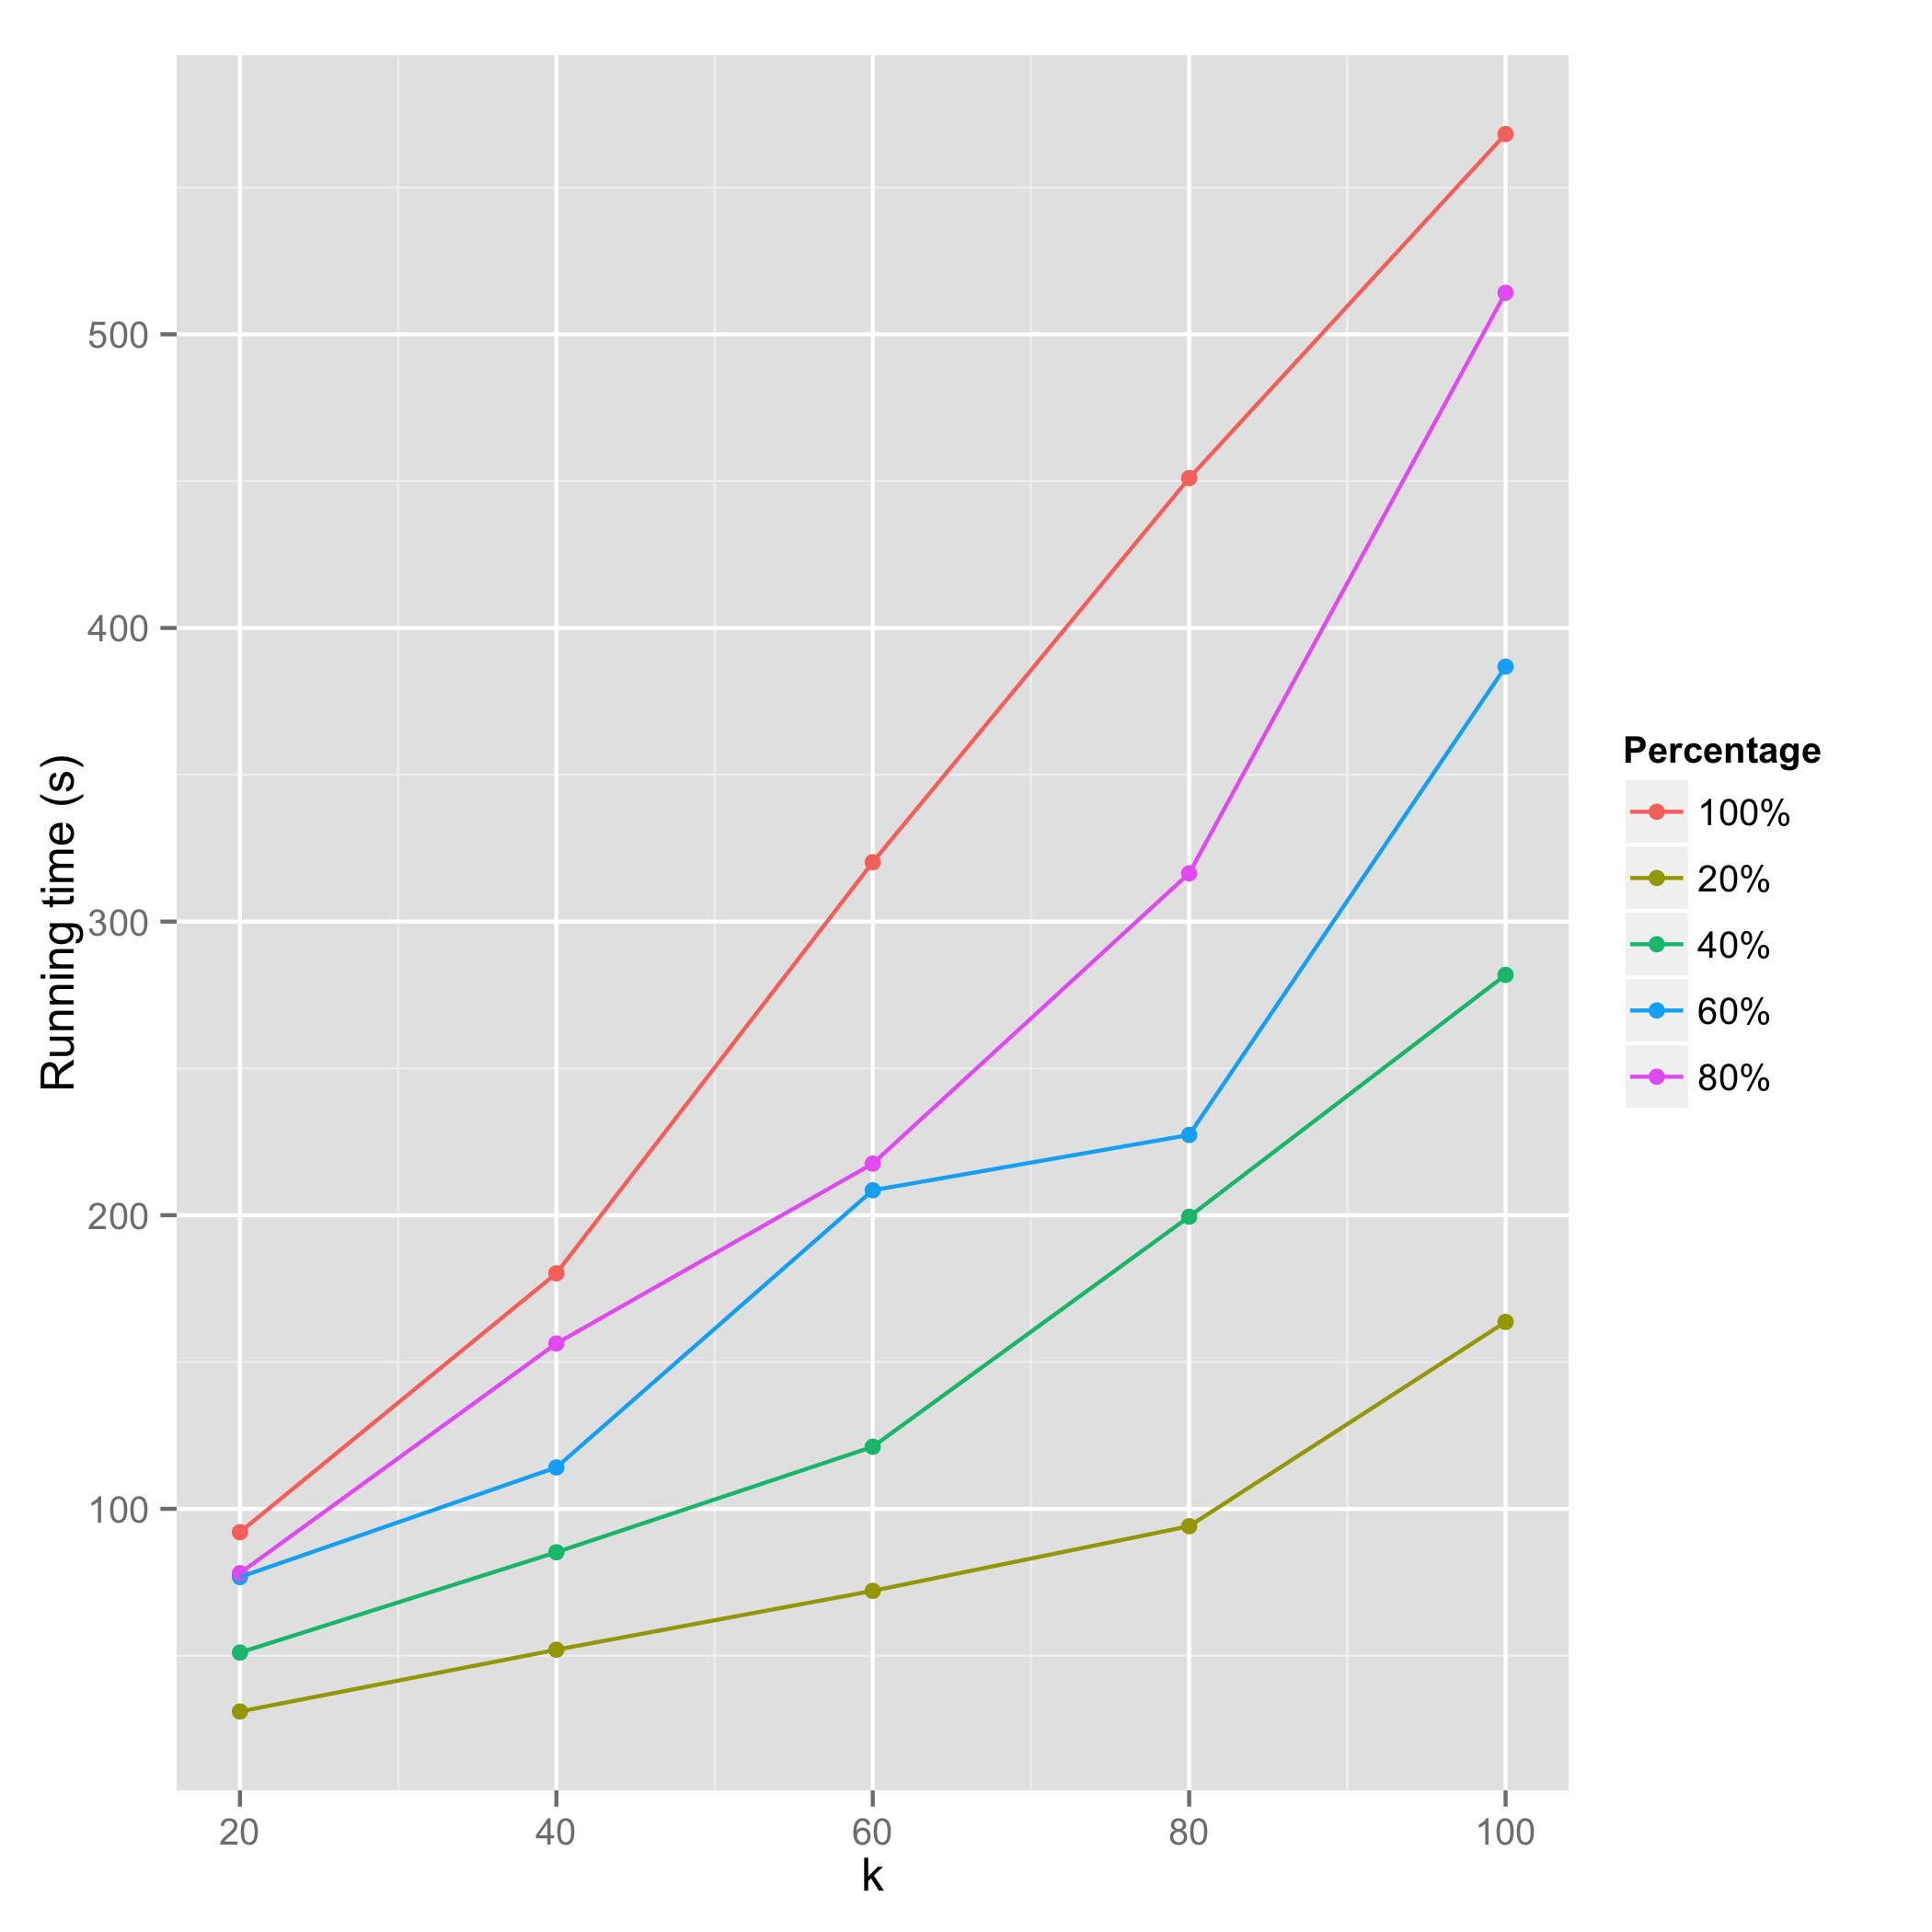
\includegraphics[width=0.7\textwidth]{lda_dim.png}
  \centering
  \caption{Running time for various percentages of data points}
  \label{fig:lda-dim}
\end{figure}

Finally, \autoref{fig:emr-runtime-lda} shows how the running time decreases as
more worker nodes are added to the cluster. We can see a definite decrease in
the slope, even more clearly than in the corresponding experiment when running
k-means.

\begin{figure}[htbp]
  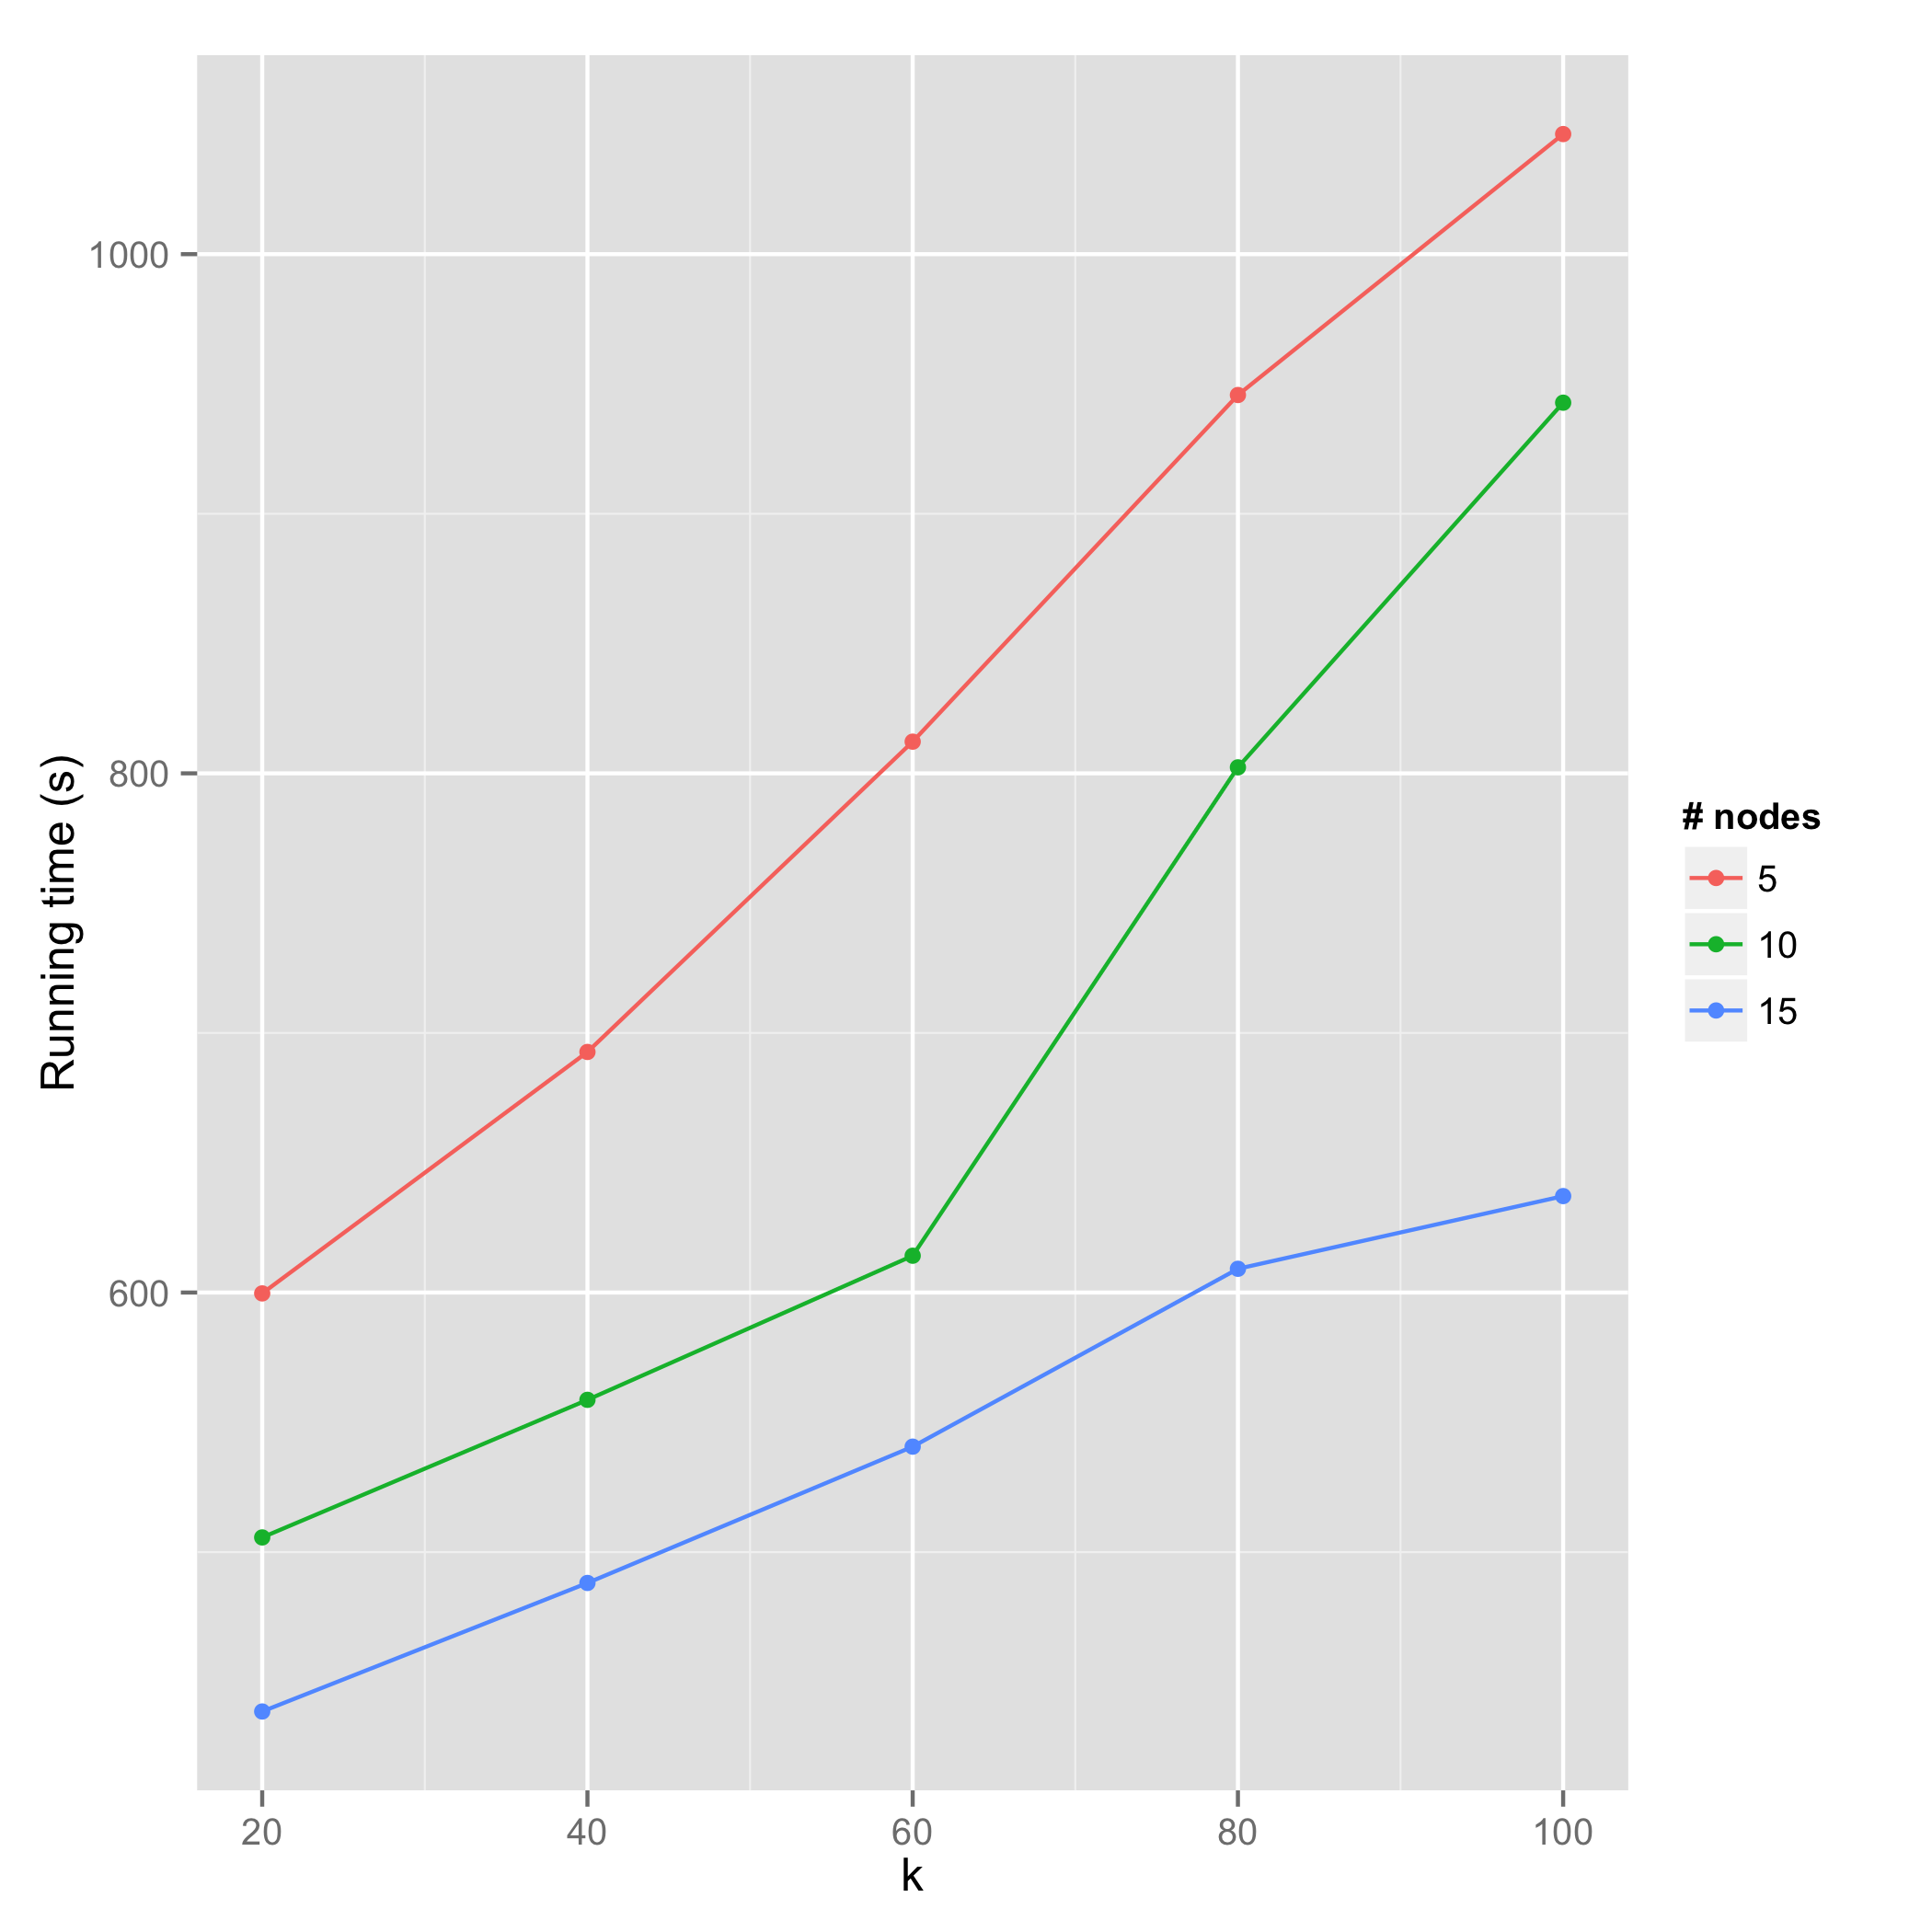
\includegraphics[width=0.7\textwidth]{running_times_emr_lda.png}
  \centering
  \caption{Running time for various amount of worker nodes}
  \label{fig:emr-runtime-lda}
\end{figure}

\subsection{Final clustering}
As done for the k-means clustering, we inspect the outcome manually. Running
the algorithm and setting the number of topics to 30 as previously discussed
the topics listed in appendix \ref{app:lastfmlda} emerges along with their
top three associated words. The weight of the tag in this context is the
probability of certain tag in the topic, $P(word | topic)$. Optimally, for the
purposes of this thesis, these topics would correspond to genres of music. This
is true for some of the topics, such as topics 6, 7, 10, 14, et.c. Others are a
bit more mixed. Such as topic 3, which has ``Classical'' mixed in with ``soul''
and ``rnb''.

The algorithm also outputs the probability of an artist's tag coming from a
certain topic, $P(topic | artist)$. Combining these we can see which are the
most likely topics for the artists we used in the k-means evaluation. For
simplicitys sake the topics are represented by their id but also the name of 
their highest weighted tag. \autoref{tbl:lastfmlda} lists the same artists as
listed after running K-means in the previous section.

\begin{table}[h]
  \centering
  \begin{tabular}{ |l|l|l| }
  \hline
  Artist name & Top topics & Topic probability \\
  \hline
  \multirow{4}{*}{The Rolling Stones} & 15 - classic rock & 0.770 \\
   & 7 - rock & 0.127 \\
   & 16 - seen live & 0.041 \\
   & 14 - indie & 0.030 \\

  \hline

  \multirow{4}{*}{Bob Dylan} & 29 - singer-songwriter & 0.583 \\
   & 15 - classic rock & 0.324 \\
   & 16 - seen live & 0.055 \\
   & 7 - rock & 0.013 \\

  \hline

  \multirow{4}{*}{Madonna} & 3 - pop & 0.664 \\
   & 11 - female vocalists & 0.149 \\
   & 26 - dance & 0.109 \\
   & 6 - electronic & 0.034 \\

  \hline

  \multirow{4}{*}{Frank Sinatra} & 22 - jazz & 0.835 \\
   & 3 - pop & 0.082 \\
   & 15 - classic rock & 0.080 \\
   & 14 - indie & 0.014 \\

  \hline

  \multirow{4}{*}{Antonio Vivaldi} & 18 - soul & 0.965 \\
   & 22 - jazz & 0.020 \\
   & 28 - punk & 0.002 \\
   & 5 - ambient & 0.002 \\

  \hline

  \multirow{4}{*}{Eminem} & 23 - Hip-Hop & 0.830 \\
   & 3 - pop & 0.050 \\
   & 7 - rock & 0.026 \\
   & 16 - seen live & 0.023 \\

  \hline

  \end{tabular}
  \caption{LDA clustering of the Last.FM data set}
  \label{tbl:lastfmlda}
\end{table}

Antonio Vivaldi immedietally stands out as an anomaly. Neither ``soul'',
``jazz'' or ``punk'' would normally be used to describe Vivaldi's music. Note
however, that topic number 18 (marked here as ``soul'') is very dominant, and
the top two tags in that topic are ``soul'' (0.118) and ``Classical'' (0.108).
The latter being a much more reasonable tag for Vivaldi.

Other than that, the topics and topic probabilities the algorithm found seems
to, subjectively, be rather accurate, especially when taking note of the weights
of the topics.


\chapter{Large scale clustering}

\textit{This chapter aims to}
\begin{itemize}
\itshape
\renewcommand{\labelitemi}{$-$}
\item apply the algorithms and techniques discussed in section 2 to the Tumblr
data set, and
\item present and discuss the outcome of the clustering jobs.
\end{itemize}

\section{Preparation}
Massaging the data into Mahout's vector representation is mostly done in the
same way as described for the Last.FM data set in the previous section, with a
couple of differences.

As mentioned, serializing the dictionary and distributing it to the worker nodes
as a part of the configuration is not an option as the full dictionary is close
to one GB and the default limit is five MB. Instead, the dictionary is
distributed using Hadoop's distributed cache feature. The distributed cache is
designed to take large read-only files from HDFS and automatically cache them
on the data nodes.\cite[p.~289]{white2012hadoop}

The files from the distributed cache are read in the setup phase of the map task
and in this context it is a matter of reading the dictionary from a SequenceFile
into a Java HashMap. Unfortunately, this does not work either for the full
Tumblr data set as the reading of the dictionary from the cache takes more than
ten minutes, the default time limit for the setup phase of a map task.

Instead, I limit the amount of tags to only the two million most common ones.
This leads to a dictionary of only 42 MB. An alternative could be building the
vectors locally. That way the setup time limit would not be an issue, but the
process would of course take a lot longer than if the full cluster was used.

Another possibility could be to reduce the dimensionality by only considering
the first $n$ tags on a post, working with the hypothesis that users will use
more important (in some sense) tags first. It is unclear, however, to what kind
of decrease in dimensionality this would lead to.

\section{Spherical K-Means}
Due to the success with spherical k-means for the small scale data set it is
again used for the large scale data set. Again, $k = 60$ is used. It is a
mostly arbitrary choice. It is meant to keep it low enough to be able to get a
good overview of all clusters. The reason the elbow method is not used as
previously done for the small scale clustering is two-fold. First, the
clustering job takes up a lot of resources of the Hadoop cluster which might
interfere with other jobs that are used in production. Secondly, increasing $k$
further leads to memory usage issues as discussed in the next section.

\subsection{Performance and running time}
Even though the dimensionality of the data set was limited to two million in the
previous section to be able to actually create the feature vectors in a
MapReduce fashion, it has to be limited even more for the actual clustering.
With two million dimensions and using $k = 60$, the production cluster at Tumblr
struggles with the memory usage of the tasks on the data nodes. Running the job
in the same way as for the small scale data set the worked nodes run out of
memory since they need to keep the last couple of iterations in memory.

This could perhaps be mitigated by altering the configuration of the cluster by
allowing a fewer number of tasks per data node giving each task the possibility
to use more memory without starving the others. This, however, is not a
possibility since this is a live cluster and there are many other jobs, used in
production, that run on it.

Instead, the dimensionality is further reduced by choosing only the tags that
have been used 150 times (overall), or more. This leads to a total of 535270
tags in the dictionary, or 11.4 MB.

Running the spherical k-means algorithm with this input and keeping $k = 60$ on
the Tumblr Hadoop cluster 1 hour, 34 minutes and 46 seconds elapsed until the
convergence threshold (max 1\% of data points reassigned in an iteration) was
reached. 

\subsection{Final clustering}
In order to assess if blogs have been assigned to a fitting a cluster, some sort
of reference is needed. For this purpose, the Tumblr spotlight page will be
used.

The spotlight page is a directory of blogs divided into around 50 subjects,
curated by the Community team at Tumblr. Six blogs will be chosen from six of
these categories, and compared with the top three tags in their assigned
clusters.

\begin{table}[h]
  \centering
  \begin{tabular}{ |l|l|l| }
  \hline
  Blog name (category) & Top tags & Tag weight\\
  \hline
  \multirow{4}{*}{Pitchfork (Music)} & music & 0.204 \\
   & rock & 0.013 \\
   & the & 0.012 \\
   & video & 0 \\

  \hline
  \multirow{4}{*}{The Getty (Art)} & art & 0.165 \\
   & illustration & 0.068 \\
   & drawing & 0.058 \\
   & anime & 0.035 \\

  \hline
  \multirow{4}{*}{Engineering is Awesome (Science)} & architecture & 0.054 \\
   & gaming & 0.034 \\
   & education & 0.027 \\
   & history & 0.024 \\

  \hline
  \multirow{4}{*}{BBC One (Television)} & sherlock & 0.192 \\
   & doctor & 0.115 \\
   & who & 0.071 \\
   & spoilers & 0.059 \\

  \hline
  \multirow{4}{*}{Olympics (Sports)} & boanoite & 0.064 \\
   & feliz & 0.048 \\
   & goodmorning & 0.038 \\
   & amigos & 0.029 \\

  \hline
  \multirow{4}{*}{Vogue (Fashion)} & fashion & 0.214 \\
   & polyvore & 0.122 \\
   & style & 0.094 \\
   & model & 0.024 \\

  \hline

  \end{tabular}
  \caption{Output of K-means clustering on the Tumblr data set}
  \label{tbl:tumblrkmeans}
\end{table}

Looking at \autoref{tbl:tumblrkmeans}, There are a couple of assignments that
stand out as a bit odd. The first being the Olympics blog belonging to a cluster
with a centroid with portuguese and spanish tags. This could possibly be due the
fact that the next summer olympics will be held in Brazil. The second assignment
that seems a bit odd is the ``Engineering is awesome'' blog, with the top tags
``architecture'', ``gaming'', ``education'' and ``history''. Overall, this
cluster seems to cover a lot of academic subjects and given that the blog is in
the ``Science'' category the cluster assignment might not be as odd as initially
thought. The cluster ``BBC One'' is assigned to also is dominated by tags one
might not have expected, until you consider that ``Sherlock'' and ``Doctor Who''
are TV shows from the BBC that have very large followings on Tumblr.

In the small scale test the six initial artists and their cluster assignments
were compared with six additional, similar, artists to see whether they ended up
in the same clusters or not. The same thing is done here but choosing the
additional blogs from the same category and shown in \autoref{tbl:tumblrcompare}

\begin{table}
  \centering
  \begin{tabular}{ |l|l|l|l| }
  \hline
  Category & Blog \#1 & Blog \#2 & Same cluster? \\
  \hline
  Music & Pitchfork & Rolling Stone & Yes \\
  Art & The Getty & SFMOMA & Yes \\
  Science & Engineering is awesome & Atomic-o-licious & Yes \\  
  Television & BBC One & Zap-2-It & No \\
  Sports & Olympics & Yahoo Sports & No \\
  Fashion & Vogue & Harper's Bazaar & Yes \\
  \hline
  \end{tabular}
  \caption{Comparing cluster assignment of blogs in same category}
  \label{tbl:tumblrcompare}
\end{table}

The fact that the ``Olympics'' and ``Yahoo Sports'' blogs did not end up in the
same cluster can probably be explained with the fact that ``Olympics'' was
assigned to the cluster with portuguese and spanish tags, as seen earlier.
Finally, ``Zap-2-It'' belongs to a cluster with top tags ``supernatural'',
``spn'', ``teen'', and ``wolf''. Supernatural and Teen Wolf are two american TV
shows, that also have large followings on Tumblr.

The average size of the clusters is 194 206.7 data points, with a standard
deviation of 200 264.6. The smallest cluster contains 47 230 data points, while
the largest contains 1 570 229. As was the case with the small scale test, the 
cluster sizes vary quite heavily.

\section{Latent Dirichlet Allocation}
LDA showed good results in the small scale test. Both in terms of scaling with
the number of worker nodes used and with the results. For the large scale test,
the number of topics is kept at 30.

In the first run of this job, no stopword filtering was applied. The result was
that ``the'' was one of the most likely tag in almost every topic, closely
followed by other very high frequent words. Stopword filtering is suggested by
Blei, Ng and Jordan (2003) in the paper introducing LDA.\cite{blei2003lda} The
results presented in this section are the results of the running the LDA
algorithm after removing a set of stopwords. The stopwords chosen were the
standard list from Lucene with a couple of additions based on frequent tags seen
in the initial attempt. The full list of stopwords can be found in the source
code. Please see appendix \ref{app:source}.

\subsection{Performance and running time}
The same, reduced, data set used in with spherical K-means was used for LDA as
well and no other memory issues appeared. One thing to note is that to be able
to run the Mahout LDA implementation on the Tumblr Hadoop cluster the Mahout
package used had to be updated to very latest, in which (so far experimental)
support for Hadoop 2.x is present. This upgrade might enable more efficient
usage of the cluster compared with previous LDA jobs which ran on an older version
of Hadoop.

The job took 2 hours, 39 minutes and 37 seconds to complete.

\subsection{Final clustering}
Looking over the topics found (see appendix \ref{app:tumblrlda}) there are some
topics that look coherent while others are less. There are two topics, topics
\#9 and \#28, that are centered on fashion.  One of them focussing more on
Polyvore, a social commerce site with a focus on fashion. There is also a clear
photography topic, topic \#23, where ``photography'', ``black'' and ``white''
are important tags.

Interesting to note is also that K-means found a single cluster that
contained the TV shows ``Doctor Who'', ``Sherlock'' and ``Supernatural'' while
LDA split these up into separate topics. Namely topics \#14, \#18 and \#16
respectively. 

Other topics are not so coherent. Topic \#21 for example, with the top three
tags ``art'', ``cute'' and ``cats''. Other topics have tags which maybe should
have been added to the stopwords list. Such as topic \#8 with top tags ``like'',
``just'' and ``have''.

In order to see the topics LDA found were prominent for each blog we reuse the
blogs chosen for evaluating the result of the previous K-means job here as well.
Again, we present this by listing the top four topics for each blog and the most
common tag in those topics in \autoref{tbl:tumblrlda}.

\begin{table}[h]
  \centering
  \begin{tabular}{ |l|l|l| }
  \hline
  Blog name (category) & Top topics & Topic probability \\
  \hline
  \multirow{4}{*}{Pitchfork (Music)} & 23 - photography & 0.386 \\
   & 9 - fashion & 0.187 \\
   & 26 - news  & 0.145 \\
   & 20 - queued & 0.087 \\

  \hline

  \multirow{4}{*}{The Getty (Art)} & 23 - photography & 0.773 \\
   & 26 - news & 0.123 \\
   & 21 - art & 0.060 \\
   & 9 - fashion & 0.015 \\

  \hline

  \multirow{4}{*}{Engineering is awesome (Science)} & 26 - news & 0.808 \\
   & 23 - photography & 0.135 \\
   & 1 - snk & 0.030 \\
   & 18 - sherlock & 0.006 \\

  \hline

  \multirow{4}{*}{BBC One (Television)} & 18 - sherlock & 0.389 \\
   & 14 - doctor & 0.268 \\
   & 27 - harry & 0.087 \\
   & 23 - photography & 0.087  \\

  \hline

  \multirow{4}{*}{Olympics (Sports)} & 26 - news & 0.571 \\
   & 29 - ifttt & 0.162 \\
   & 24 - exo & 0.120 \\
   & 5 - love & 0.031 \\

  \hline

  \multirow{4}{*}{Vogue (Fashion)} & 9 - fashion & 0.739 \\
   & 28 - polyvore & 0.158 \\
   & 14 - doctor & 0.053 \\
   & 26 - news & 0.014 \\

  \hline

  \end{tabular}
  \caption{LDA clustering of the Tumblr data set}
  \label{tbl:tumblrlda}
\end{table}

``The Getty'' and, especially, ``Vogue'' seem to have mixtures of topic that
suit them. ``BBC One'' does too when, although the topic with ``harry'' seems a
bit out of place. Overall, the topic mixtures for the various blogs seem
relatively good, but not quite as good as the small scale test.

\chapter{Conclusions}

\textit{This chapter aims to}
\begin{itemize}
\itshape
\renewcommand{\labelitemi}{$-$}
\item summarize and draw conclusions about the scalability from the small scale 
and large scale tests,
\item discuss the quality of the clusterings, and
\item briefly discuss possible use-cases and improvements
\end{itemize}

\section{Scalability and performance}
We saw that both algorithms work nicely with the small scale data set (which is
an actual, real-world data set), even on a single computer. They both seemed to
scale roughly linearly with the amount of worker nodes in use. LDA showing more
consistent running times than K-means.

Going in to the project, I thought that the algorithms would be mostly CPU
bound. This turned out to be false when moving on to the large scale data set as
significant reductions in dimensionality had to be made in order to solve memory
problems. These issues also put a limit on the choice of $k$ for k-means. It is
possible that these issues can be mitigated by a more liberal configuration of
memory related parameters, both in my code and the Hadoop cluster configuration.
The ``mapred.child.java.opts'' setting allows for increasing the maximum heap
size of map and reduce tasks, but increasing might impact other tasks.
Furthermore, this setting is already set quite high on the Tumblr hadoop
cluster.

There were also a couple of problems when transforming the data into vectors
for Mahout. This is unrelated to the performance of the algorithms, but still a
problem that needs to be taken in to consideration in practice. In order to
create vectors we need to have a dictionary which map each tag to a unique
integer (the index in the vector) and the dictionary needs to be available to
all worker nodes. In the small scale test this was trivial as the dictionary was
small enough to send with the job configuration. 

For the large scale tests the dictionary was distributed using Hadoop's
distributed cache, and the dictionary was read by each task when starting.
Initially, the tasks took too long reading the dictionary, hitting the time
limit for the setup phase of the tasks causing them to fail. This was ultimately
resolved by further reduction of dimensionality leading to a smaller dictionary.
It is possible this could be solved by altering the ``mapred.task.timeout''
parameter (default 600 seconds) to allow the tasks more time to load the
dictionary. This would however tie up a lot of task slots for a long time.
Another option would be to generate the vectors offline (i.e. not using Hadoop). 
This would of course take longer time, but that might be a tradeoff worth doing 
if removing dimensions is not an option.

In conclusion, Mahout can definitely handle data sets with a cardinality in the
tens of millions of data points. However, a natural language data set of this
size will most likely have too many dimensions for a default Hadoop cluster to
handle memory-wise. In this thesis, this has been circumvented by only including
the most common tags. In a real environment we would probably limit our
dictionary both by setting a cut-off point for the number of times a tag has
been used but also more aggressive stopword filtering, preferrably with a
stopword list specific to the data set as well.

\section{Cluster quality}
Attempting a high-quality clustering is not the primary goal of this thesis.
Nevertheless, since we are performing a series of clusterings we might as well
se what kind of results come out.

During the small scale tests, k-means showed good results. The artists chosen
were assigned to clusters with appropriate tag weights. For instance, the top
tags of the cluster ``Eminem'' was assigned are all variations on ``hip-hop'' or
``rap''. There also seems to be a nicely defined cluster around the tag
``Classical'' (weight 0.762), which ``Antonio Vivaldi'' was assigned to. When
investigating whether similar artists are assigned to the same cluster or not,
only one couple did not; ``Madonna''and ``Kylie Minogue''. As mentioned
previously, this is likely due to the strong influence of the ``australian'' tag 
for ``Kylie Minogue''. This suggests that we might want to filter out non-music 
related tags, in the case we are strictly interested in genres and such. These 
country-related tags can also be seen by looking at the full cluster output.
There are quite a few clusters where tags like ``finnish'', ``deutsch'' or
``japanese'' have heavy weights. This is, of course, specific to the Last.FM
data set, and while filtering these out in subsequent clustering jobs might be
benificial here that might not be the case for other data sets.  Since the
quality of the clustering was not the primary goal in this project this
filtering was not performed.

LDA also worked fairly well for the small scale test, although some of the
topics seem to consist of mixed genres. For instance, topic \#18 has, as
mentioned before, ``soul'', ``classical'' and ``rnb'' as the three most probable
tags. Again, we see a few topics with language tags in them.

For the large scale K-means clustering we saw that blogs chosen from the
Discovery page were assigned to clusters centered around relevant tags. Similar
blogs were assigned to the same clusters, with the exception of blogs from the
Television section and the Sports section. Possible reasons for this was
discussed in section 5.5.2. Looking at the full K-means output of the large
scale clustering we are able to find some of the subcultures (or fandoms, in
Tumblr lingo) one might expect to see on Tumblr. For instance, clusters \#2, 
\#17 and \#45 seem to revolve around television shows; The Vampire Diaries,
Supernatural and Doctor Who. Cluster \#47 appears to be a ``Youtube-cluster''
with tags representing popular Youtubers. A couple of music-related clusters
appear (\#35 - 5 Seconds of Summer, \#55 - One Direction and \#56 - Justin
Bieber). The fact that these subcultures were split in to disctinct clusters to
me shows a succesful clustering. There are however some problems. Tags such as
``http'' and ``com'' do not really add anything and are most likely from
automated posting from other sites such as IFTTT or Instagram.

The latent topics found by LDA in the Tumblr data set are not quite as clear as
the clusters found by K-means. Again, we see topics centered around TV-shows
(\#14 - Doctor Who, \#16 - Supernatural, \#18 - Sherlock). However, there are a
couple of topics that are either non-sensical (e.g. \#22 with tags ``oh'',
``yes'' and ``love'') or seem to consist of varying tags (e.g. \#12 with tags
``disney'', ``food'' and ``fitness'').

\section{Future improvements and use-cases}
In both the cases with spherical K-means and LDA the data sets could probably
have used some filtering in terms of stopwords (which was already used to some
extent for LDA) and imposing harder limits on how many times a tag has to be
used before including it to make the data less noisy, especially in the case of
the Tumblr data set since the tags were split in to unigrams and is used more as 
an extension of the post instead of categorization, which I believe is more the
case with tags in the Last.FM data set. 

The output from the clustering jobs is most likely not something that can be
consumed by end-users immedietally. It might however be useful as input to other
algorithms. For example, using the assignment of the cluster as a feature in a
recommendation engine or for classification. Blei, Ng and Jordan (2003) gives
the example of using LDA for document classification by training a support
vector machine using the model inferred by using LDA. They achieve the same (and
sometimes even better) results with a 99.6\% reduction in feature
space.\cite{blei2003lda}

For spherical K-means tf/idf weighting was used which seems to have generated
good results. Wilson and Chew (2010) suggest adding a weighting scheme to LDA as
well, in the process eliminating the need for stopword filtering.
\cite{wilson2010term} This would be interesting to explore, as it might give the
benefits of a weighting scheme while also taking in to account correlations.

Overall, I consider the experiments a success. Mahout has shown to scale nicely
with the computing power available but also some problematic issues with memory
usage became apparent. It is indeed capable of clustering very large data sets
but, and in especially the case with Tumblr, quite heavy filtering might be
needed, as well as term weighting. Both for reducing the memory resources needed
and trying to filter out noisy data.

\bibliography{references}{}
\bibliographystyle{ieeetr}

\begin{appendices}
\chapter{Git repository of source code and data}
\label{app:source}
Link to github and explanation of repo layout goes here.

\chapter{Full clustering outputs}
In this appendix section are lists of the centroids from K means and the topics
from LDA clusterings.

\section{Last.FM Spherical K-Means output}
\label{app:lastfmkmeans}
The following table shows the three most prominent tags for each of the 60
centroids the spherical k-means algorithm found.

\begingroup
  \fontsize{8pt}{10pt}\selectfont
  \begin{verbatim}
Centroid 0:  german 0.188            deutsch 0.097             Hawaiian 0.096
Centroid 1:  synthpop 0.194          80s 0.183                 new wave 0.145
Centroid 2:  noise 0.236             breakcore 0.192           deathrock 0.166
Centroid 3:  norwegian 0.398         danish 0.353              norsk 0.115
Centroid 4:  folk 0.244              Czech 0.119               singer-songwriter 0.084
Centroid 5:  Hip-Hop 0.317           hip hop 0.199             rap 0.146
Centroid 6:  post-punk 0.181         Garage Rock 0.157         New Zealand 0.058
Centroid 7:  Avant-Garde 0.211       experimental 0.192        contemporary classical 0.099
Centroid 8:  jazz 0.422              swing 0.109               oldies 0.063
Centroid 9:  twee 0.241              indie pop 0.223           swedish 0.096
Centroid 10: classic rock 0.120      rock 0.079                russian 0.067
Centroid 11: Progressive metal 0.359 metal 0.121               Nu Metal 0.115
Centroid 12: pop punk 0.204          emo 0.177                 punk 0.086
Centroid 13: italian 0.234           latin 0.179               brazilian 0.170
Centroid 14: screamo 0.428           post-hardcore 0.166       emo 0.157
Centroid 15: christian 0.758         christian rock 0.201      worship 0.193
Centroid 16: funk 0.283              soul 0.222                Disco 0.141
Centroid 17: Belgium 0.222           belgian 0.188             slovak 0.150
Centroid 18: Drum and bass 0.175     downtempo 0.155           chillout 0.134
Centroid 19: hard rock 0.277         hair metal 0.266          glam rock 0.096
Centroid 20: video game music 0.662  Game Music 0.287          game 0.189
Centroid 21: celtic 0.797            irish 0.158               bagpipes 0.149
Centroid 22: psychobilly 0.958       rockabilly 0.530          horror punk 0.244
Centroid 23: Soundtrack 0.464        anime 0.130               musicals 0.121
Centroid 24: thrash metal 0.499      Melodic Death Metal 0.428 death metal 0.150
Centroid 25: dutch 0.262             Nederlandstalig 0.202     chinese 0.139
Centroid 26: Power metal 0.716       folk metal 0.219          heavy metal 0.155
Centroid 27: RAC 0.926               nsbm 0.276                vikingarock 0.171
Centroid 28: eurobeat 0.232          female vocalists 0.188    singer-songwriter 0.090
Centroid 29: j-pop 0.374             japanese 0.295            JPop 0.263
Centroid 30: techno 0.542            podcast 0.143             schranz 0.081
Centroid 31: world 0.265             turkish 0.259             african 0.112
Centroid 32: comedy 0.711            funny 0.126               humor 0.101
Centroid 33: blues 0.295             jazz 0.231                Romanian 0.087
Centroid 34: post-rock 0.268         spanish 0.223             Spanish Rock 0.091
Centroid 35: irish 0.326             acoustic 0.176            Irish Folk 0.064
Centroid 36: finnish 0.644           Suomi 0.070               seen live 0.070
Centroid 37: doom metal 0.377        Gothic Metal 0.312        Gothic 0.135
Centroid 38: hardcore 0.362          metalcore 0.212           polish 0.170
Centroid 39: trance 0.411            dance 0.169               House 0.162
Centroid 40: heavy metal 0.217       Canadian 0.206            hard rock 0.115
Centroid 41: Crust 0.447             anarcho-punk 0.309        folk punk 0.160
Centroid 42: industrial 0.360        ebm 0.310                 darkwave 0.135
Centroid 43: Sludge 0.220            drone 0.150               Stoner Rock 0.129
Centroid 44: black metal 0.779       Progressive rock 0.182    melodic black metal 0.070
Centroid 45: death metal 0.433       grindcore 0.217           swedish 0.215
Centroid 46: french 0.491            chanson francaise 0.201   Surf 0.110
Centroid 47: rap 0.368               Hip-Hop 0.208             hip hop 0.146
Centroid 48: reggae 0.399            dancehall 0.201           rnb 0.200
Centroid 49: shoegaze 0.437          dream pop 0.129           4ad 0.072
Centroid 50: idm 0.179               electronic 0.149          minimal 0.097
Centroid 51: punk 0.218              ska 0.186                 punk rock 0.104
Centroid 52: australian 0.522        Aussie 0.149              New Zealand 0.102
Centroid 53: Classical 0.523         new age 0.160             piano 0.104
Centroid 54: indie 0.128             indie rock 0.100          seen live 0.052
Centroid 55: OC ReMix 0.617          game remixes 0.412        video game music 0.318
Centroid 56: splatterpop 0.851       great german Rock 0.550   Aschaffenburg 0.511
Centroid 57: country 0.808           bluegrass 0.180           Alt-country 0.087
Centroid 58: japanese 0.354          J-rock 0.353              visual kei 0.199
Centroid 59: Flamenco 0.313          guitar virtuoso 0.264     guitar 0.190
  \end{verbatim}
\endgroup

\section{Last.FM LDA topic output}
\label{app:lastfmlda}
These are the topics from the final LDA clustering job with their three most
prominent tags.
\begingroup
  \fontsize{8pt}{10pt}\selectfont
  \begin{verbatim}
Topic 0:  post-rock 0.166         experimental 0.158      doom metal 0.098
Topic 1:  finnish 0.154	          french 0.094            comedy 0.065
Topic 2:  Power metal 0.192       Gothic Metal 0.140      metal 0.125
Topic 3:  pop 0.412               80s 0.073               rock 0.045
Topic 4:  Progressive metal 0.201 ska 0.138               reggae 0.134
Topic 5:  ambient 0.147           psychedelic 0.052       new age 0.048
Topic 6:  electronic 0.304        electronica 0.143       idm 0.052
Topic 7:  rock 0.310              alternative 0.197       alternative rock 0.12
Topic 8:  seen live 0.247         Canadian 0.105          swedish 0.103
Topic 9:  german 0.131            ebm 0.097               Gothic 0.065
Topic 10: metal 0.260             heavy metal 0.192       Melodic Death Metal 0.136
Topic 11: female vocalists 0.448  female 0.066            female vocalist 0.038
Topic 12: indie 0.145             indie pop 0.129         Soundtrack 0.077
Topic 13: japanese 0.174          j-pop 0.091             JPop 0.062
Topic 14: indie 0.332             indie rock 0.173        alternative 0.12
Topic 15: classic rock 0.214      rock 0.168              Progressive rock 0.1
Topic 16: seen live 0.243         rock 0.158              emo 0.137
Topic 17: death metal 0.348       thrash metal 0.129      grindcore 0.092
Topic 18: soul 0.118              Classical 0.108         rnb 0.074
Topic 19: metal 0.191             rock 0.163              hard rock 0.101
Topic 20: Grunge 0.284            Stoner Rock 0.121       rock 0.099
Topic 21: hardcore 0.245          metalcore 0.156         screamo 0.107
Topic 22: jazz 0.338              blues 0.065             Fusion 0.03
Topic 23: Hip-Hop 0.283           rap 0.166               hip hop 0.134
Topic 24: punk 0.305              punk rock 0.115         new wave 0.085
Topic 25: trip-hop 0.152          chillout 0.151          downtempo 0.085
Topic 26: dance 0.203             trance 0.147            House 0.09
Topic 27: industrial 0.313        industrial metal 0.089  seen live 0.064
Topic 28: black metal 0.406       folk metal 0.112        viking metal 0.063
Topic 29: singer-songwriter 0.244 folk 0.199              acoustic 0.072
  \end{verbatim}
\endgroup

\section{Tumblr Spherical K-Means output}
\label{app:tumblrkmeans}
This section presents the centroids found in the Tumblr data set by K-means.
\begingroup
  \fontsize{8pt}{10pt}\selectfont
  \begin{verbatim}
Centroid 0:  bitstrips 0.152      ifttt 0.144        meus 0.138
Centroid 1:  black 0.098          pokemon 0.095      white 0.084
Centroid 2:  tvd 0.073            vampire 0.055      damon 0.036
Centroid 3:  architecture 0.054   gaming 0.034       education 0.028
Centroid 4:  girl 0.101           hair 0.067         grunge 0.033
Centroid 5:  rp 0.364             roleplay 0.110     rpg 0.101
Centroid 6:  tattoo 0.217         lt3 0.161          tattoos 0.11
Centroid 7:  http 0.779           com 0.264          www 0.236
Centroid 8:  spotify 1.144        music 0.505        text 0.119
Centroid 9:  liebe 0.109          berlin 0.081       ich 0.066
Centroid 10: graffiti 0.044       cara 0.038         delevingne 0.024
Centroid 11: beach 0.151          diary 0.151        journal 0.106
Centroid 12: dog 0.105            fall 0.058         puppy 0.056
Centroid 13: kik 0.303            selfie 0.241       bored 0.074
Centroid 14: family 0.090         daddy 0.065        dom 0.032
Centroid 15: chicago 0.033        san 0.026          california 0.026
Centroid 16: quotes 0.360         fave 0.058         audio 0.046
Centroid 17: supernatural 0.103   spn 0.078          teen 0.055
Centroid 18: food 0.160           foodporn 0.044     yummy 0.04
Centroid 19: of 0.102             zelda 0.022        thrones 0.017
Centroid 20: milestone 0.597      posts 0.571        tumblr 0.335
Centroid 21: homestuck 0.080      snk 0.075          no 0.035
Centroid 22: me 0.314             fav 0.051          1d 0.018
Centroid 23: music 0.204          rock 0.013         the 0.012
Centroid 24: webcamtoy 1.465      effect 0.850       acnl 0.184
Centroid 25: exo 0.302            kpop 0.068         sehun 0.065
Centroid 26: love 0.155           you 0.000          true 0.0
Centroid 27: this 0.033           is 0.023           you 0.0
Centroid 28: de 0.088             la 0.040           bestfriend 0.024
Centroid 29: friends 0.154        party 0.045        best 0.042
Centroid 30: art 0.165            illustration 0.068 drawing 0.058
Centroid 31: photography 0.246    landscape 0.027    35mm 0.021
Centroid 32: cat 0.186            cats 0.089         kitten 0.04
Centroid 33: personal 0.441       the 0.009          thoughts 0.0
Centroid 34: gifboom 0.325        gif 0.294          mine 0.195
Centroid 35: summer 0.124         5sos 0.115         luke 0.056
Centroid 36: follow 0.437         back 0.082         f4f 0.079
Centroid 37: amor 0.292           frases 0.202       para 0.08
Centroid 38: tumblr 0.508         milestone 0.354    birthday 0.179
Centroid 39: boanoite 0.065       feliz 0.048        goodmorning 0.038
Centroid 40: birthday 0.656       tumblr 0.401       happy 0.032
Centroid 41: eu 0.079             amore 0.073        que 0.066
Centroid 42: fitness 0.18         fitblr 0.104       healthy 0.093
Centroid 43: lol 0.127            funny 0.091        cute 0.084
Centroid 44: poetry 0.182         quote 0.154        writing 0.107
Centroid 45: sherlock 0.192       doctor 0.115       who 0.071
Centroid 46: fashion 0.214        polyvore 0.122     style 0.094
Centroid 47: danisnotonfire 0.097 amazingphil 0.058  oakley 0.048
Centroid 48: tbt 0.148            weed 0.089         nofilter 0.072
Centroid 49: the 0.07             sims 0.026         ts3 0.0
Centroid 50: depression 0.124     depressed 0.064    suicide 0.062
Centroid 51: pink 0.105           nails 0.071        flowers 0.052
Centroid 52: sad 0.088            help 0.058         sorry 0.041
Centroid 53: 2013 0.174           truth 0.055        watch 0.042
Centroid 54: design 0.121         payday 0.063       loan 0.062
Centroid 55: harry 0.097          styles 0.073       direction 0.052
Centroid 56: justin 0.178         bieber 0.173       icons 0.137
Centroid 57: swag 0.205           dope 0.084         yolo 0.074
Centroid 58: gay 0.083            sex 0.081          porn 0.059
Centroid 59: new 0.095            halloween 0.066    york 0.042
  \end{verbatim}
\endgroup

\section{Tumblr LDA topic output}
\label{app:tumblrlda}
The topics from the final LDA clustering job of the Tumblr data set with their
three most prominent tags.
\begingroup
  \fontsize{8pt}{10pt}\selectfont
  \begin{verbatim}
Topic 0:  photo 0.056       reblog 0.054       breaking 0.005
Topic 1:  snk 0.028         free 0.027         anime 0.023
Topic 2:  girl 0.061        sexy 0.046         girls 0.044
Topic 3:  follow 0.084      love 0.054         quotes 0.036
Topic 4:  rp 0.081          hs 0.033           roleplay 0.0192
Topic 5:  love 0.018        selfie 0.006       tattoo 0.006
Topic 6:  nsfw 0.104        gay 0.088          porn 0.060
Topic 7:  sex 0.043         ass 0.042          porn 0.039
Topic 8:  like 0.017        just 0.015         have 0.012
Topic 9:  fashion 0.077     style 0.015        design 0.011
Topic 10: tom 0.019         potter 0.017       hp 0.015
Topic 11: chat 0.030        cam 0.016          5sos 0.014
Topic 12: disney 0.028      food 0.021         fitness 0.017
Topic 13: dont 0.013        fuck 0.013         like 0.0113
Topic 14: doctor 0.042      who 0.033          teen 0.0170
Topic 15: lol 0.031         homestuck 0.025    funny 0.0185
Topic 16: spn 0.077         supernatural 0.070 dean 0.043
Topic 17: ronpa 0.021       dangan 0.020       aph 0.019
Topic 18: sherlock 0.122    spoilers 0.044     benedict 0.022
Topic 19: personal 0.031    ooc 0.013          dont 0.011
Topic 20: queued 0.036      glee 0.029         wolf 0.019
Topic 21: art 0.054         cute 0.029         cats 0.014
Topic 22: oh 0.0165         yes 0.013          love 0.013
Topic 23: photography 0.028 black 0.024        white 0.021
Topic 24: exo 0.057         sehun 0.013        kai 0.012
Topic 25: text 0.047        fav 0.021          love 0.020
Topic 26: news 0.020        boys 0.007         men 0.007
Topic 27: harry 0.061       one 0.046          direction 0.038
Topic 28: polyvore 0.055    fashion 0.046      style 0.036
Topic 29: ifttt 0.162       instagram 0.069    com 0.037
  \end{verbatim}
\endgroup
\end{appendices}

\end{document}
